\documentclass[journal]{IEEEtran}

\usepackage{cite}
\usepackage{amsmath,amssymb}
\usepackage{graphicx}
\setkeys{Gin}{draft=false}
\usepackage{booktabs}
\usepackage{multirow}
\usepackage{url}
\usepackage{hyperref}
\usepackage{enumitem}
\usepackage{algorithm}
\usepackage{algorithmic}
\usepackage{float}

\begin{document}

\title{KG-Hybrid: A Knowledge-Guided Trustworthy AI Framework for Robust Crop Recommendation}

\author{
\IEEEauthorblockN{
G. Sai Sagar,
M. Guna Varshith,
T. V. Tarun Kumar,
Rinku Rani Das
}
}

\maketitle

\begin{abstract}

Crop recommendation is an important process in the field of precision agriculture and helps in choosing the right crop types using the soil and environmental conditions. The current frameworks utilize conventional machine learning or deep learning approaches where the agriculture data is considered as generic tabular data ignoring the agricultural domain knowledge. In addition, the current models behave like black-box models, offering predictions without any explanation or confidence score.

In this paper, we introduce the novel \textbf{Knowledge-Guided Trustworthy AI Framework} for intelligent crop recommendation, which considers soil information, climate conditions, and environmental features in a single learning paradigm. As the key component of the proposed framework, we present the \textbf{Knowledge-Guided Agriculture-Aware Attention Network (KGAAN)}, which combines the leaf embeddings from XGBoost and FT-Transformer using the knowledge-guided gated fusion approach, taking into account the agricultural domain knowledge.

We test our framework on an agricultural benchmark dataset, comparing it against six competing models. Our framework scores 99.70\% accuracy, beating XGBoost (99.39\%) and FT-Transformer (98.79\%). Ablation study with seven different settings is conducted to show the significance of every single component in our framework. The results of robustness test show that the proposed framework outperforms others in terms of Gaussian noise ($89.21\%$ for $\sigma=0.2$) and feature extrapolation ($90.00\%$ for $\times 1.5$). For practical application, we combine KNN imputation (40\% missing feature accuracy improved to 82.73\%), confidence-aware early exit (inference time reduced to 5.99 ms), and light-weight network structure (parameters reduced by 74\% to 4.04M).

\end{abstract}

\begin{IEEEkeywords} 
Crop Recommendation, Precision Farming, Trustworthy Artificial Intelligence, Explainable Artificial Intelligence, Knowledge-Guided Learning, Hybrid Learning
\end{IEEEkeywords}
\section{Introduction}

Agriculture is crucial to ensuring food security, economic development, and efficient use of natural resources. One of the most important tasks in agriculture is the selection of appropriate crops, which influences the efficiency, usage of natural resources, and profits of farms. The suitability of certain crops is determined by various factors that interact together, such as soil nutrients, pH, temperature, humidity, precipitation, and seasons. With the growing amount of data on agriculture and advances in AI technologies, crop recommendation systems became popular decision-making tools for the selection of crops according to environmental and soil conditions.

\subsection{Motivation and Challenges}

Despite recent advances in AI-powered crop recommendation, there are a number of challenges preventing the usage of these algorithms in practice.

\textbf{Insufficient Utilization of Agronomical Information:}
The majority of existing models treat agricultural knowledge as regular tabular data and focus on statistical patterns that can be learned using the provided samples.

\textbf{Interpretability Issues:}
A number of machine learning algorithms and deep learning algorithms predict crops but do not have the capacity to explain the reasoning behind their recommendation. This could make it difficult for farmers and agricultural experts to verify whether or not the recommendation is appropriate for a specific field.

\textbf{No Measurement of Uncertainty:}
Environmental factors related to agriculture might change because of different weather conditions, sensor noise, and variation in the soil properties. A prediction without any estimation of uncertainty will not be able to tell how reliable the recommendation is in such situations.

\textbf{Deployment Problems:}
Deep learning algorithms might need a significant amount of computation power and memory that makes deployment in agricultural settings a bit hard. Apart from that, real-world sensor data might have missing values that will need to be dealt with before prediction.

These limitations show that we need a framework for recommending crops that can combine knowledge about agriculture with data-driven learning while being interpretable and deployable.

\subsection{Proposed Framework and Contributions}

This paper presents \textbf{KG-Hybrid}, a \textbf{Knowledge-Guided Trustworthy AI Framework} for crop recommendation that integrates soil, climate, and environmental data into a single learning framework. \textbf{KGAAN (Knowledge-Guided Agriculture-Aware Attention Network)}, which constitutes the core of this framework, has the following contributions:

\begin{enumerate}
    \item \textbf{Agricultural knowledge integration:} Learnable knowledge matrix, obtained by the guidelines of FAO and ICAR on agriculture, is employed to guide the interactions and representation learning of features.

    \item \textbf{Integration of complementary models:} XGBoost leaf embedding learns decision boundaries and local patterns, while FT-Transformer captures interactions among input features. Both of them are integrated using a knowledge-guided gated fusion approach.

    \item \textbf{Explanation:} SHAP based feature importance scores are utilized to discover the features responsible for crop recommendations.

    \item \textbf{Uncertainty estimation:} Monte Carlo dropout is used to estimate the uncertainty level in predictions and calculate confidence scores. Safety alert can be issued when the uncertainty is above a pre-specified threshold.

    \item \textbf{Practicality:} KNN imputation is performed to deal with missing features, while confidence-based early exit scheme and lightweight network structure are presented to decrease inference cost.
\end{enumerate}

The key novelties of this work are summarized below:

\begin{enumerate}
    \item \textbf{Knowledge-Guided Hybrid Architecture:} KG-Hybrid unites XGBoost leaf embeddings and FT-Transformer representations through a knowledge-guided gated fusion technique which makes it possible to use agricultural knowledge in the learning process.

    \item \textbf{Interpretability and Uncertainty Estimation:} SHAP-based feature importance and Monte Carlo Dropout techniques are used to provide interpretative recommendations along with uncertainty estimation.

    \item \textbf{Enhanced Predictive Performance:} KG-Hybrid is able to reach 99.70\% accuracy on the benchmark dataset for crop recommendation task, while the accuracy achieved by XGBoost and FT-Transformer equals 99.39\% and 98.79\% respectively. Ablation experiments are employed to test the contribution of individual components of the proposed framework.

    \item \textbf{Enhanced Robustness:} Under Gaussian noise ($\sigma=0.2$) KG-Hybrid reaches 89.21\% accuracy, while XGBoost achieves 79.39\%. Under feature extrapolation ($\times 1.5$ scaling) KG-Hybrid achieves 90.00\% accuracy, while the accuracy achieved by XGBoost and Random Forest equals 74.55\% and 80.00\% respectively.

    \item \textbf{Efficient Deployment:} The accuracy of KNN imputation is 82.73\% under 40\% feature dropout. Confidence-based early exit reduces the reported inference time to 5.99 ms, while the lightweight network reduces the parameter count by 74\% to 4.04M.
\end{enumerate}

\subsection{Paper Structure}

The rest of the paper is structured as follows. Section II provides a literature survey of previous work on crop recommendation systems, involving approaches based on traditional techniques, machine learning, deep learning, transformers, knowledge guidance, and explainable AI. Section III introduces the proposed KG-Hybrid framework, with its construction of knowledge matrices, embedding XGBoost leaves, FT-Transformer architecture, knowledge-guided fusion and auxiliary learning tasks. Section IV provides details of experiments, comparison to baselines and ablation studies. Section V analyzes robustness to missing values, noise and feature extrapolation. Section VI presents deployment-oriented components of KG-Hybrid: KNN imputation, early exit policy, lightweight architecture and uncertainty estimation. Section VII discusses results, limitations and future works. Finally, section VIII concludes the paper.

\section{Related Work}

In this section we review the crop recommendation research in four different areas: (1) traditional and rule-based crop recommendation, (2) machine learning-based recommendation, (3) deep learning and transformer-based crop recommendation, (4) knowledge-guided and explainable AI for crop recommendation. Later we identify the problems that are addressed by KG-Hybrid framework.

\subsection{Traditional and Rule-Based Crop Recommendation Systems}

The traditional crop recommendation systems mainly exploited expert knowledge and rules. Expert systems and fuzzy logic were utilized to express the connections between soil and climatic conditions and possible crops. In \cite{singhal2025state}, Singhal et al.~reviewed the state-of-the-art crop recommendation technology solutions and provided the overview of their application cases, benefits, challenges and perspectives. The review of crop recommendation systems within the scope of Agriculture 4.0 was done by Mancer et al.~in \cite{mancer2025systematic}.

Fuzzy logic has also been utilized for agriculture decision-making as it could represent the uncertainties regarding soil and climatic conditions. One recent comprehensive review on fuzzy expert systems for region-specific crop recommendations has considered the application of fuzzy expert systems in dealing with uncertainties in soil and environment conditions~\cite{fuzzy2026comprehensive}. Despite the interpretability nature of the fuzzy systems approach, the problem with its scalability is due to the necessity to define rules manually.

\subsection{Crop Recommendation Using Machine Learning}

Machine learning techniques allow crop recommendation systems to learn relationships between agricultural data directly. SivaGanesh et al.~\cite{sivaganesh2026machine} conducted a survey of machine learning approaches which used such features as soil nutrients, pH, temperature, humidity, and rainfall. Gamya et al.~\cite{gamya2025comparative} reviewed commonly used algorithms in crop recommendation systems, such as Decision Trees (DT), Random Forest (RF), Support Vector Machines (SVM), k-Nearest Neighbors (KNN), and Artificial Neural Networks (ANN).

Ensemble tree methods, including Random Forest and XGBoost, have proven to be efficient tools for crop recommendation. Reddy et al.~\cite{reddy2025comparative} made a comparison between Decision Trees, Random Forest, and XGBoost and outlined the benefits of XGBoost in crop prediction. Comparison of RF, SVM, and XGBoost for crop recommendation using soil-related features was another example of an efficient algorithm~\cite{xgboost2026comparative}.

However, traditional machine learning models usually learn from the values of the features without integrating any agronomical relations. The lack of usage of domain knowledge in traditional machine learning techniques is emphasized by SivaGanesh et al.~\cite{sivaganesh2026machine} and Gamya et al.~\cite{gamya2025comparative}. Traditional machine learning models make deterministic predictions without calculating the uncertainty.

Phull et al.~\cite{phull2025advances} made a survey about recent applications of machine learning and deep learning techniques, including Random Forest, SVM, CNN, and LSTM models for crop recommendation and yield prediction. The survey concludes that hybrid and interpretable models can increase both the predictive performance and the explainability.

\subsection{Deep Learning and Transformer-Based Models}

Deep learning models offer an additional level of complexity in order to learn patterns in agricultural data. Chettri et al.~\cite{chettri2026deep} reviewed deep learning models that are used in precision agriculture and include CNNs, LSTMs, Transformers, and other models for crop yield prediction and similar tasks. A survey of the application of AI for crop recommendation and soil analysis was conducted in order to analyze both machine learning and deep learning models and problems related to the prediction accuracy, computation costs, and explainability~\cite{ai2024comprehensive}.

The Transformer architecture has recently been applied to agriculture. Xie et al.~\cite{xie2024recent} reviewed the application of Transformer models to different agricultural tasks, which included crop yield prediction, plant disease detection, and livestock-related problems. The FT-Transformer architecture~\cite{gorishniy2021revisiting} is a variation of the Transformer model for tabular data representation, where the individual features are converted into embeddings and interactions between features are modeled with self-attention mechanism. Recent benchmarking studies showed that the FT-Transformer is able to compete with gradient boosting models on tabular classification tasks~\cite{fttransformer2026benchmarking}.

Nevertheless, these models may be hard to interpret owing to the complexity of their internal representations. For example, Xie et al.~\cite{xie2024recent} address this interpretability problem in the context of agricultural applications. Besides, the FT-Transformer benchmark mentions an inference time of 19.11 ms on CPU~\cite{fttransformer2026benchmarking} which could be a significant factor in some applications where fast inference is required. The computational needs of larger models complicate their deployment on resource-constrained devices~\cite{phull2025advances}.

\subsection{Knowledge-Guided and Explainable AI in Agriculture}

The use of both domain knowledge and machine learning algorithms has emerged as a new trend aimed at improving the reliability of the models and enhancing representation learning capabilities. A review of scientific knowledge and machine learning integration analyzed 143 scientific papers and classified knowledge-guided approaches according to the architecture of models and loss-function design~\cite{beyond2026data}. It was found that knowledge-guided learning remains underexplored compared to classical data-driven and hybrid approaches; only less than 25\% of analyzed studies rigorously compare the performance of knowledge-integrated models with conventional machine learning and physics-based counterparts~\cite{beyond2026data}.

Explainable AI (XAI) becomes increasingly popular in agriculture as there is a need for users to comprehend the principles of AI-generated recommendations. Thilakarathne et al.~\cite{thilakarathne2025machine} investigated the use of indigenous agricultural knowledge and machine learning for crop recommendation using mobile-based platforms. Still, frequently-used XAI techniques like SHAP produce technical explanations which may require additional interpretation to become meaningful to farmers and agricultural experts.

\subsection{Research Gaps and Motivation}

The reviewed literature highlights several gaps that motivate the development of KG-Hybrid:

\begin{enumerate}
    \item \textbf{Limited Domain-Knowledge Integration:} Existing crop recommendation models generally treat agricultural information as conventional tabular data and do not explicitly incorporate agronomic relationships. This gap is also highlighted by SivaGanesh et al.~\cite{sivaganesh2026machine}, Gamya et al.~\cite{gamya2025comparative}, and the Beyond Data-Driven review~\cite{beyond2026data}.

    \item \textbf{Limited Interpretability:} Deep learning and Transformer-based models can be difficult to interpret, while existing XAI methods may produce technical explanations that are not directly accessible to farmers~\cite{xie2024recent,thilakarathne2025machine}.

    \item \textbf{Limited Uncertainty Estimation:} The reviewed machine learning approaches generally focus on crop classification accuracy and do not explicitly provide prediction confidence or uncertainty estimates~\cite{sivaganesh2026machine,gamya2025comparative,reddy2025comparative,xgboost2026comparative}. The AI-based crop recommendation review also identifies the lack of confidence measures as a reliability concern~\cite{ai2024comprehensive}.

    \item \textbf{Deployment Constraints:} Deep learning and Transformer models can introduce additional inference time and computational requirements. For example, the FT-Transformer benchmark reported 19.11 ms CPU inference time, which may be unsuitable for some low-latency agricultural applications~\cite{fttransformer2026benchmarking}.

    \item \textbf{Limited Knowledge-Guided Hybridization:} Although hybrid models have been identified as a promising direction~\cite{chettri2026deep}, the reviewed literature does not report a crop recommendation framework that combines XGBoost leaf embeddings with Transformer-based contextual representations through an explicitly knowledge-guided fusion mechanism.
\end{enumerate}

These gaps motivate the proposed \textbf{KG-Hybrid} framework, which combines agricultural domain knowledge with complementary tree-based and Transformer-based representations while incorporating explainability, uncertainty estimation, and deployment-oriented components.
\section{Proposed Methodology}

This subsection elaborates on the proposed \textbf{KG-Hybrid} framework for crop recommendations. The methodology will describe how we formulate the problem, build the agricultural knowledge, extract dual-branch features, knowledge-guided fusion of features, auxiliary learning, training procedure, and prediction scheme.

Architecture of the KG-Hybrid framework is illustrated in Figure~\ref{fig:architecture}.

\begin{figure}[t]
    \centering
    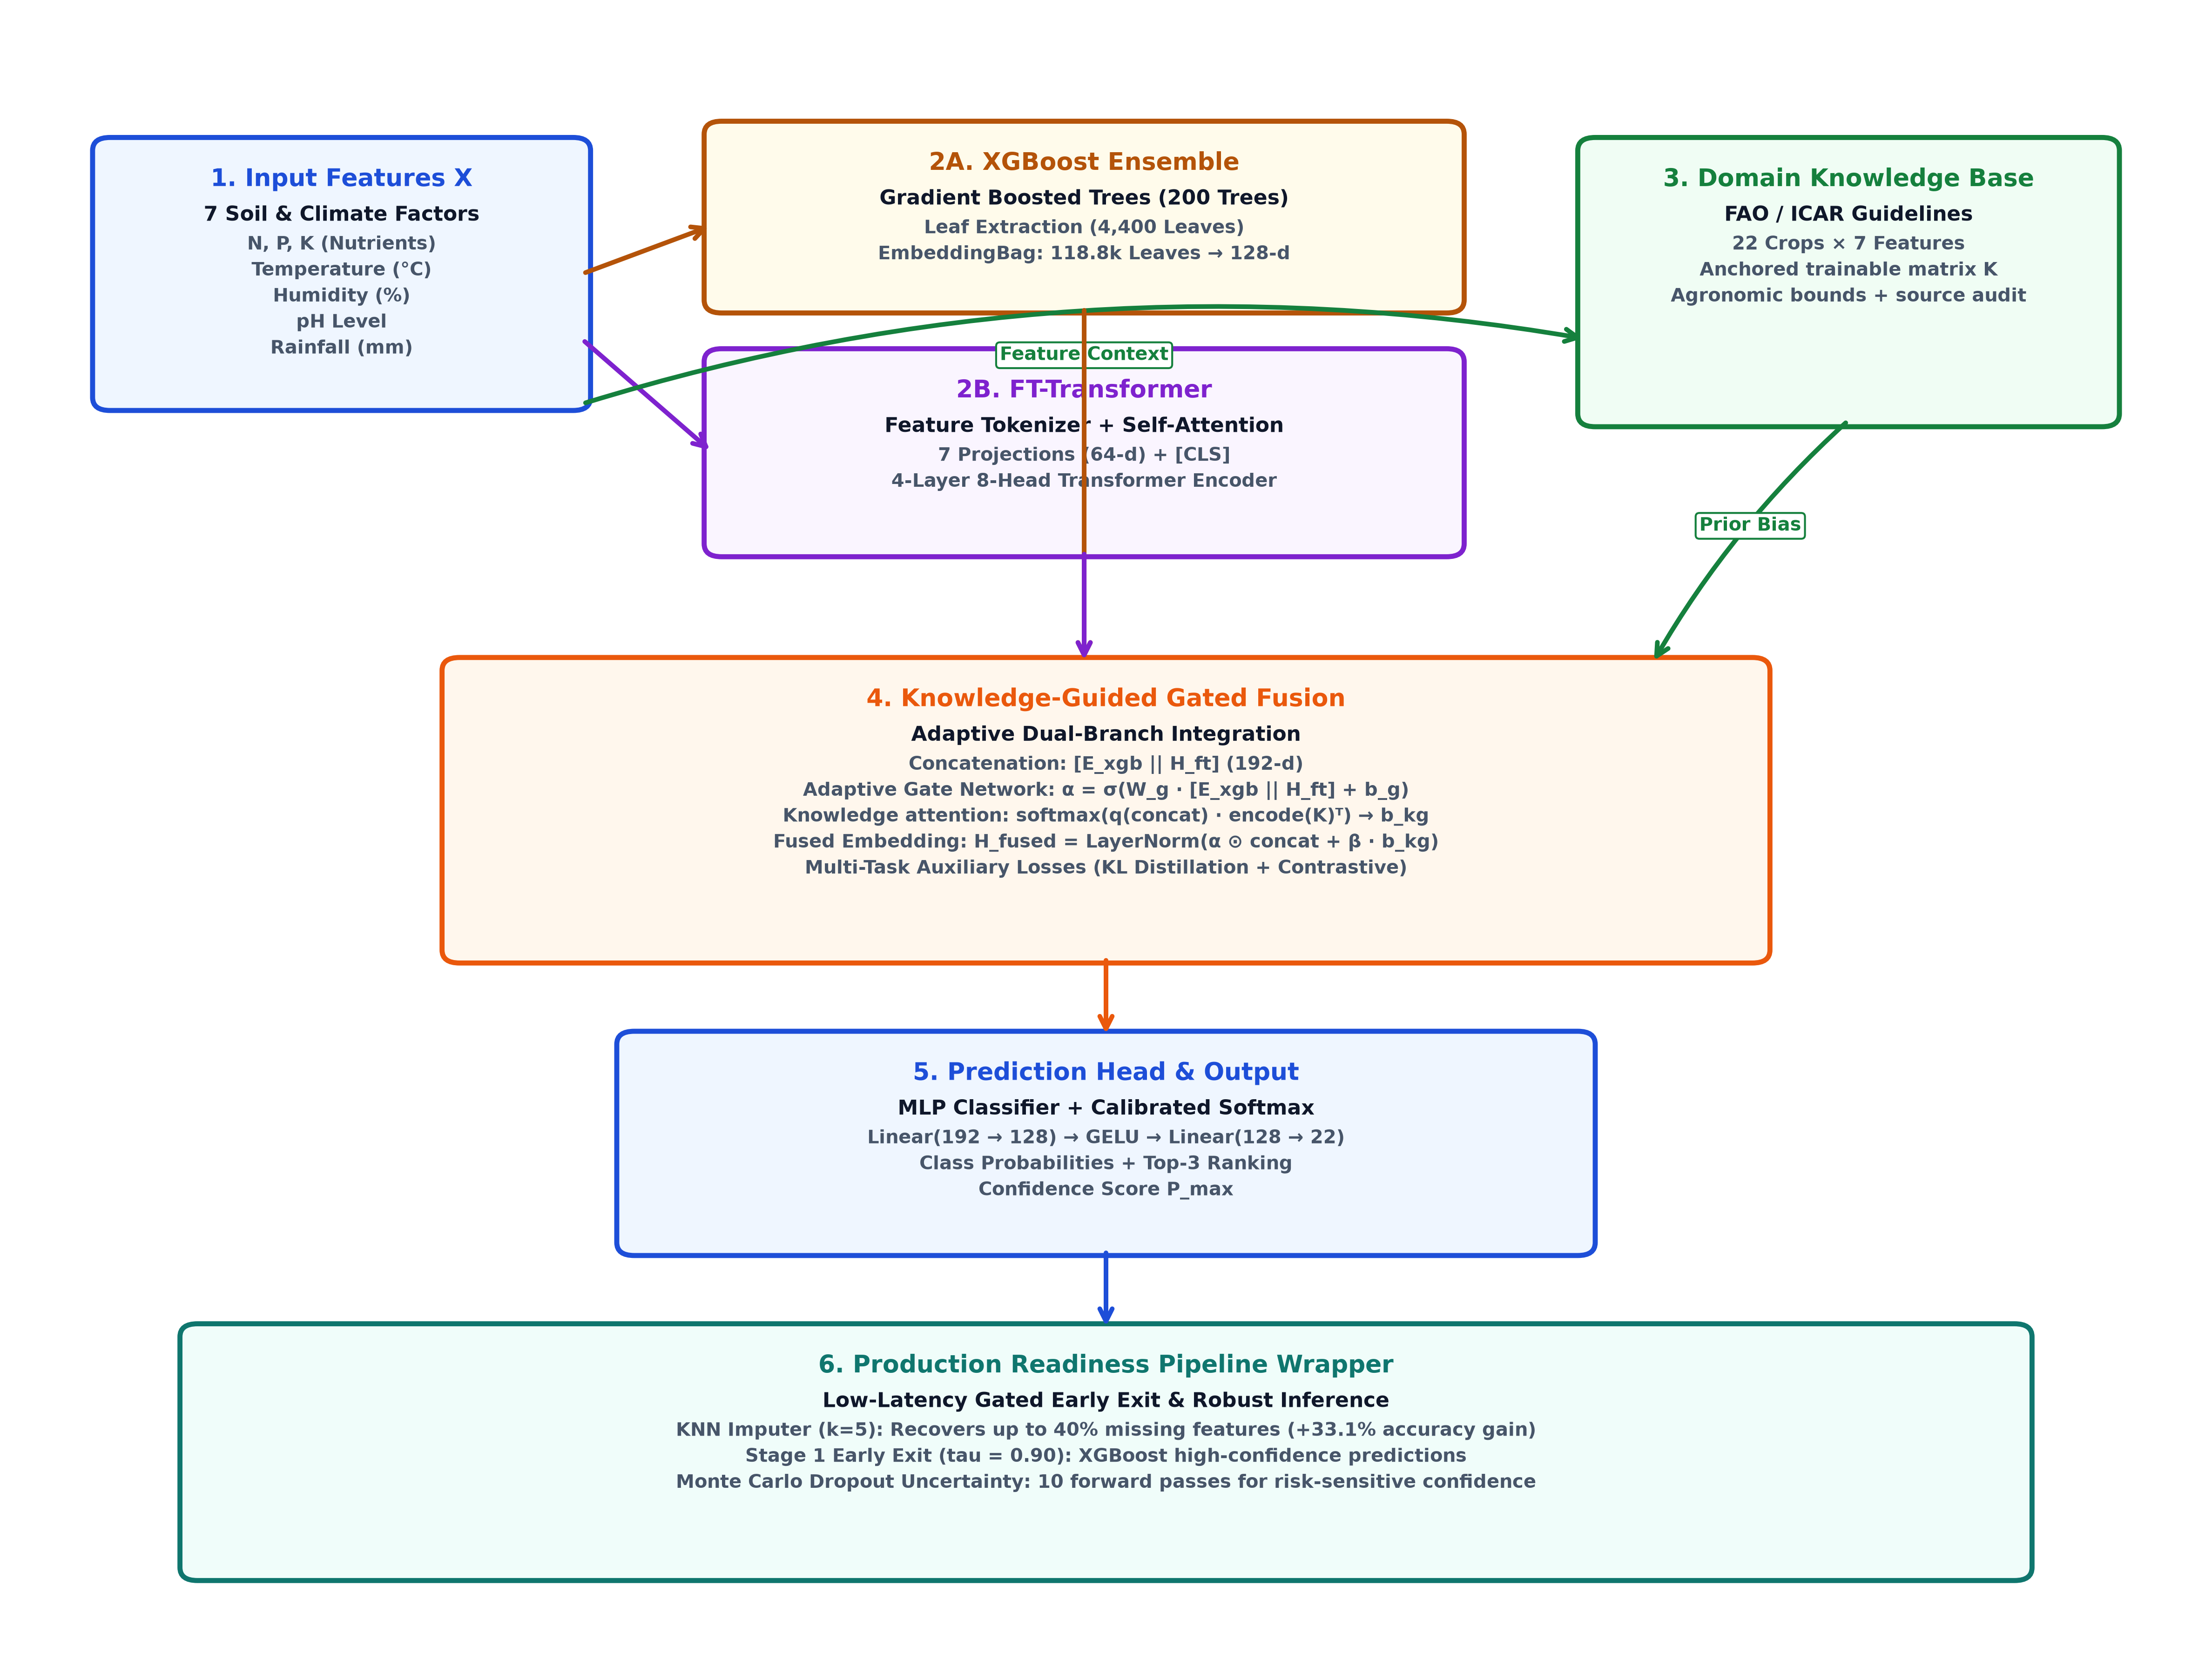
\includegraphics[
        width=\columnwidth,
        height=0.40\textheight,
        keepaspectratio
    ]{fig1_kg_hybrid_detailed_architecture.png}
    \caption{Overall architecture of the proposed KG-Hybrid framework. The framework consists of a knowledge-guided feature gate, XGBoost leaf representations, FT-Transformer features, and knowledge-guided feature fusion. The prediction head produces the recommended crop and its confidence.}
    \label{fig:architecture}
\end{figure}
\subsection{Problem Formulation}

Consider $\mathcal{D} = \{(\mathbf{x}_i, y_i)\}_{i=1}^{N}$ as a dataset having $N$ agricultural instances. An input vector $\mathbf{x}_i \in \mathbb{R}^{F}$ consists of seven agricultural variables:

\begin{equation}
\mathbf{x} =
[\text{N}, \text{P}, \text{K}, \text{temperature},
\text{humidity}, \text{pH}, \text{rainfall}]^\top
\end{equation}

where N, P, and K refer to the essential nutrients in the soil. The target

\begin{equation}
f:\mathbb{R}^{F}\rightarrow\mathcal{Y}
\end{equation}

to predict the best crop for a particular agricultural environment.

\subsection{Construction of Agricultural Knowledge}

The agricultural knowledge is embedded into the system via the knowledge matrix $\mathbf{K} \in \mathbb{R}^{C \times F}$. Each entry $K_{c,f}\in[0,1]$ indicates how well the crop $c$ fits the corresponding feature $f$; the higher the value, the better.

The initial values of the matrix entries are selected based on FAO and ICAR recommendations, expert opinion, and agronomic literature. Then, the matrix is considered as a trainable parameter that allows the model to modify the knowledge based on training data.

\begin{equation}
\mathbf{K} =
\begin{bmatrix}
K_{1,1} & K_{1,2} & \cdots & K_{1,F} \\
K_{2,1} & K_{2,2} & \cdots & K_{2,F} \\
\vdots & \vdots & \ddots & \vdots \\
K_{C,1} & K_{C,2} & \cdots & K_{C,F}
\end{bmatrix}
\end{equation}

For instance, the first representation of knowledge gives very high suitability value to the crucial conditions for crops like rice. Figure \ref{fig:knowledge_matrix} shows the entire knowledge matrix employed by the framework.

\begin{figure}[t]
    \centering
    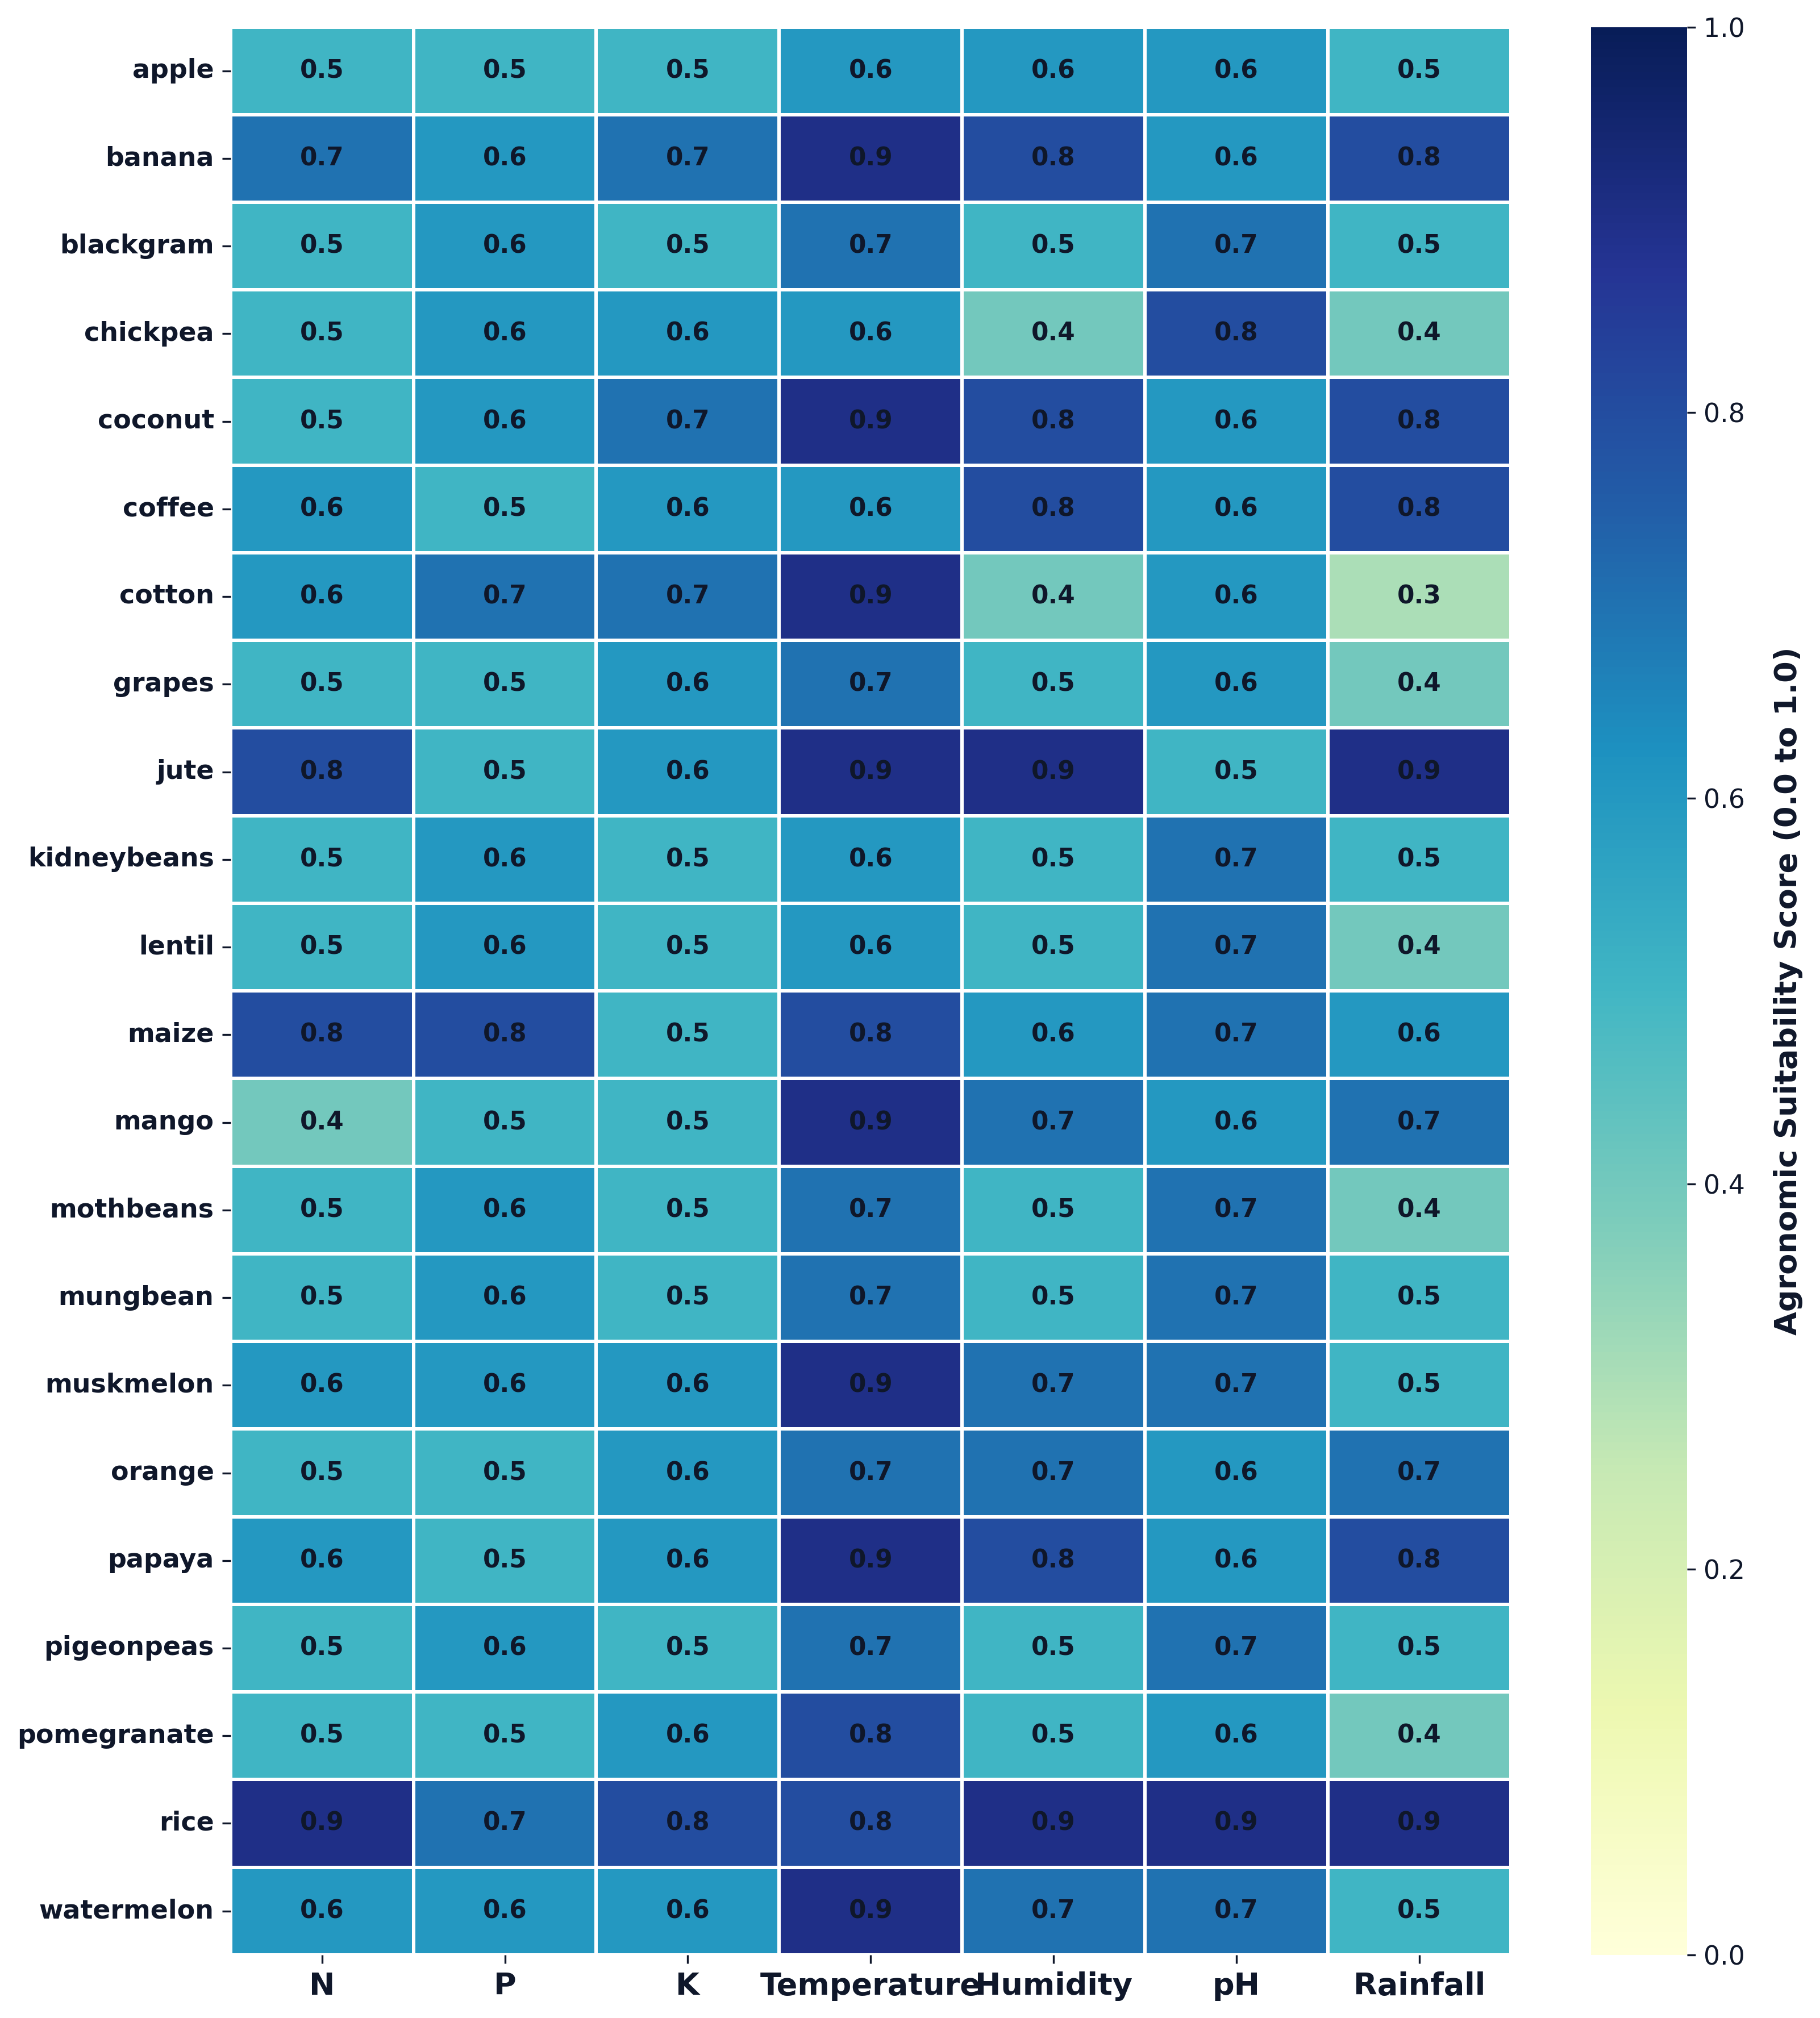
\includegraphics[width=1.0\columnwidth]{agricultural_knowledge_matrix_heatmap.png}
    \caption{Agricultural knowledge matrix $\mathbf{K}\in\mathbb{R}^{22\times7}$ crop features' suitability scores. These scores are normalized to range from [0,1] and are initially determined based on agricultural knowledge.}
    \label{fig:knowledge_matrix}
\end{figure}

\subsection{Knowledge-Guided Feature Gate}

Prior to feature extraction, a knowledge-driven gate is used to highlight features which are important in the agricultural environment. The gate is expressed by:

\begin{equation}
\mathbf{g}_{kg} =
\sigma(\mathbf{W}_g\mathbf{x}+\mathbf{b}_g+
\alpha\mathbf{K}_{c}^{\top})
\end{equation}

Where $\sigma$ is the sigmoid function, $\mathbf{W}_g$ and $\mathbf{b}_g$ are the learning parameters, $\mathbf{K}_c$ is the knowledge vector for the most likely crop and $\alpha$ is the weightage of domain knowledge.

\subsection{Branch A: XGBoost Leaf Embedding}

The first branch employs XGBoost for discovering decision-related patterns from the tabular data. The XGBoost classifier is trained on the training dataset using $T=200$ trees. Leaf index of each tree is collected from each input example.

Let $\mathbf{l}\in\mathbb{Z}^{T}$ be the corresponding leaf index vector. The indices are mapped to the trainable embeddings:

\begin{equation}
\mathbf{f}_{xgb} =
\text{EmbeddingBag}(\mathbf{l})
\in\mathbb{R}^{d_{xgb}}
\end{equation}

where the representation vectors corresponding to the leaf nodes are merged into one vector. The XGBoost classifier does not change in the hybrid training because it is used as it was already trained.

In the main model, $d_{xgb}=128$, while the lightweight version uses $d_{xgb}=32$.

\subsection{Branch B: FT-Transformer}

The second branch uses FT-Transformer~\cite{gorishniy2021revisiting} to model interactions between agricultural features.

\subsubsection{Feature Tokenizer}

Each standardized numerical feature is projected into a $d_{ft}$-dimensional embedding:

\begin{equation}
\mathbf{e}_f =
\text{Linear}(\tilde{x}_f)
\in\mathbb{R}^{d_{ft}},
\quad f=1,\ldots,F
\end{equation}

The resulting feature tokens form the sequence

\begin{equation}
\mathbf{E} =
[\mathbf{e}_1,\mathbf{e}_2,\ldots,\mathbf{e}_F]
\in\mathbb{R}^{F\times d_{ft}}.
\end{equation}

\subsubsection{CLS Token}

A learnable $[\text{CLS}]$ token is added to aggregate information from the complete feature sequence:

\begin{equation}
\mathbf{E}_{cls} =
[\mathbf{e}_{cls},\mathbf{e}_1,\ldots,\mathbf{e}_F]
\in\mathbb{R}^{(F+1)\times d_{ft}}.
\end{equation}

\subsubsection{Transformer Encoder}

The feature sequence is processed using $L=4$ Transformer encoder layers:

\begin{equation}
\mathbf{H}^{(l)} =
\text{TransformerLayer}^{(l)}
(\mathbf{H}^{(l-1)}),
\quad l=1,\ldots,L.
\end{equation}

The final $[\text{CLS}]$ representation is used as the contextual feature vector:

\begin{equation}
\mathbf{f}_{ft} =
\mathbf{H}^{(L)}_{cls}
\in\mathbb{R}^{d_{ft}}.
\end{equation}

The experiments use $d_{ft}=64$, four Transformer layers, and eight attention heads.

\subsection{Knowledge-Guided Adaptive Fusion}

The fusion component consists of the decision-based representation learned by XGBoost and the contextual representation learned by FT-Transformer. This architecture is illustrated in Figure~\ref{fig:fusion}.

\begin{figure}[t]
    \centering
    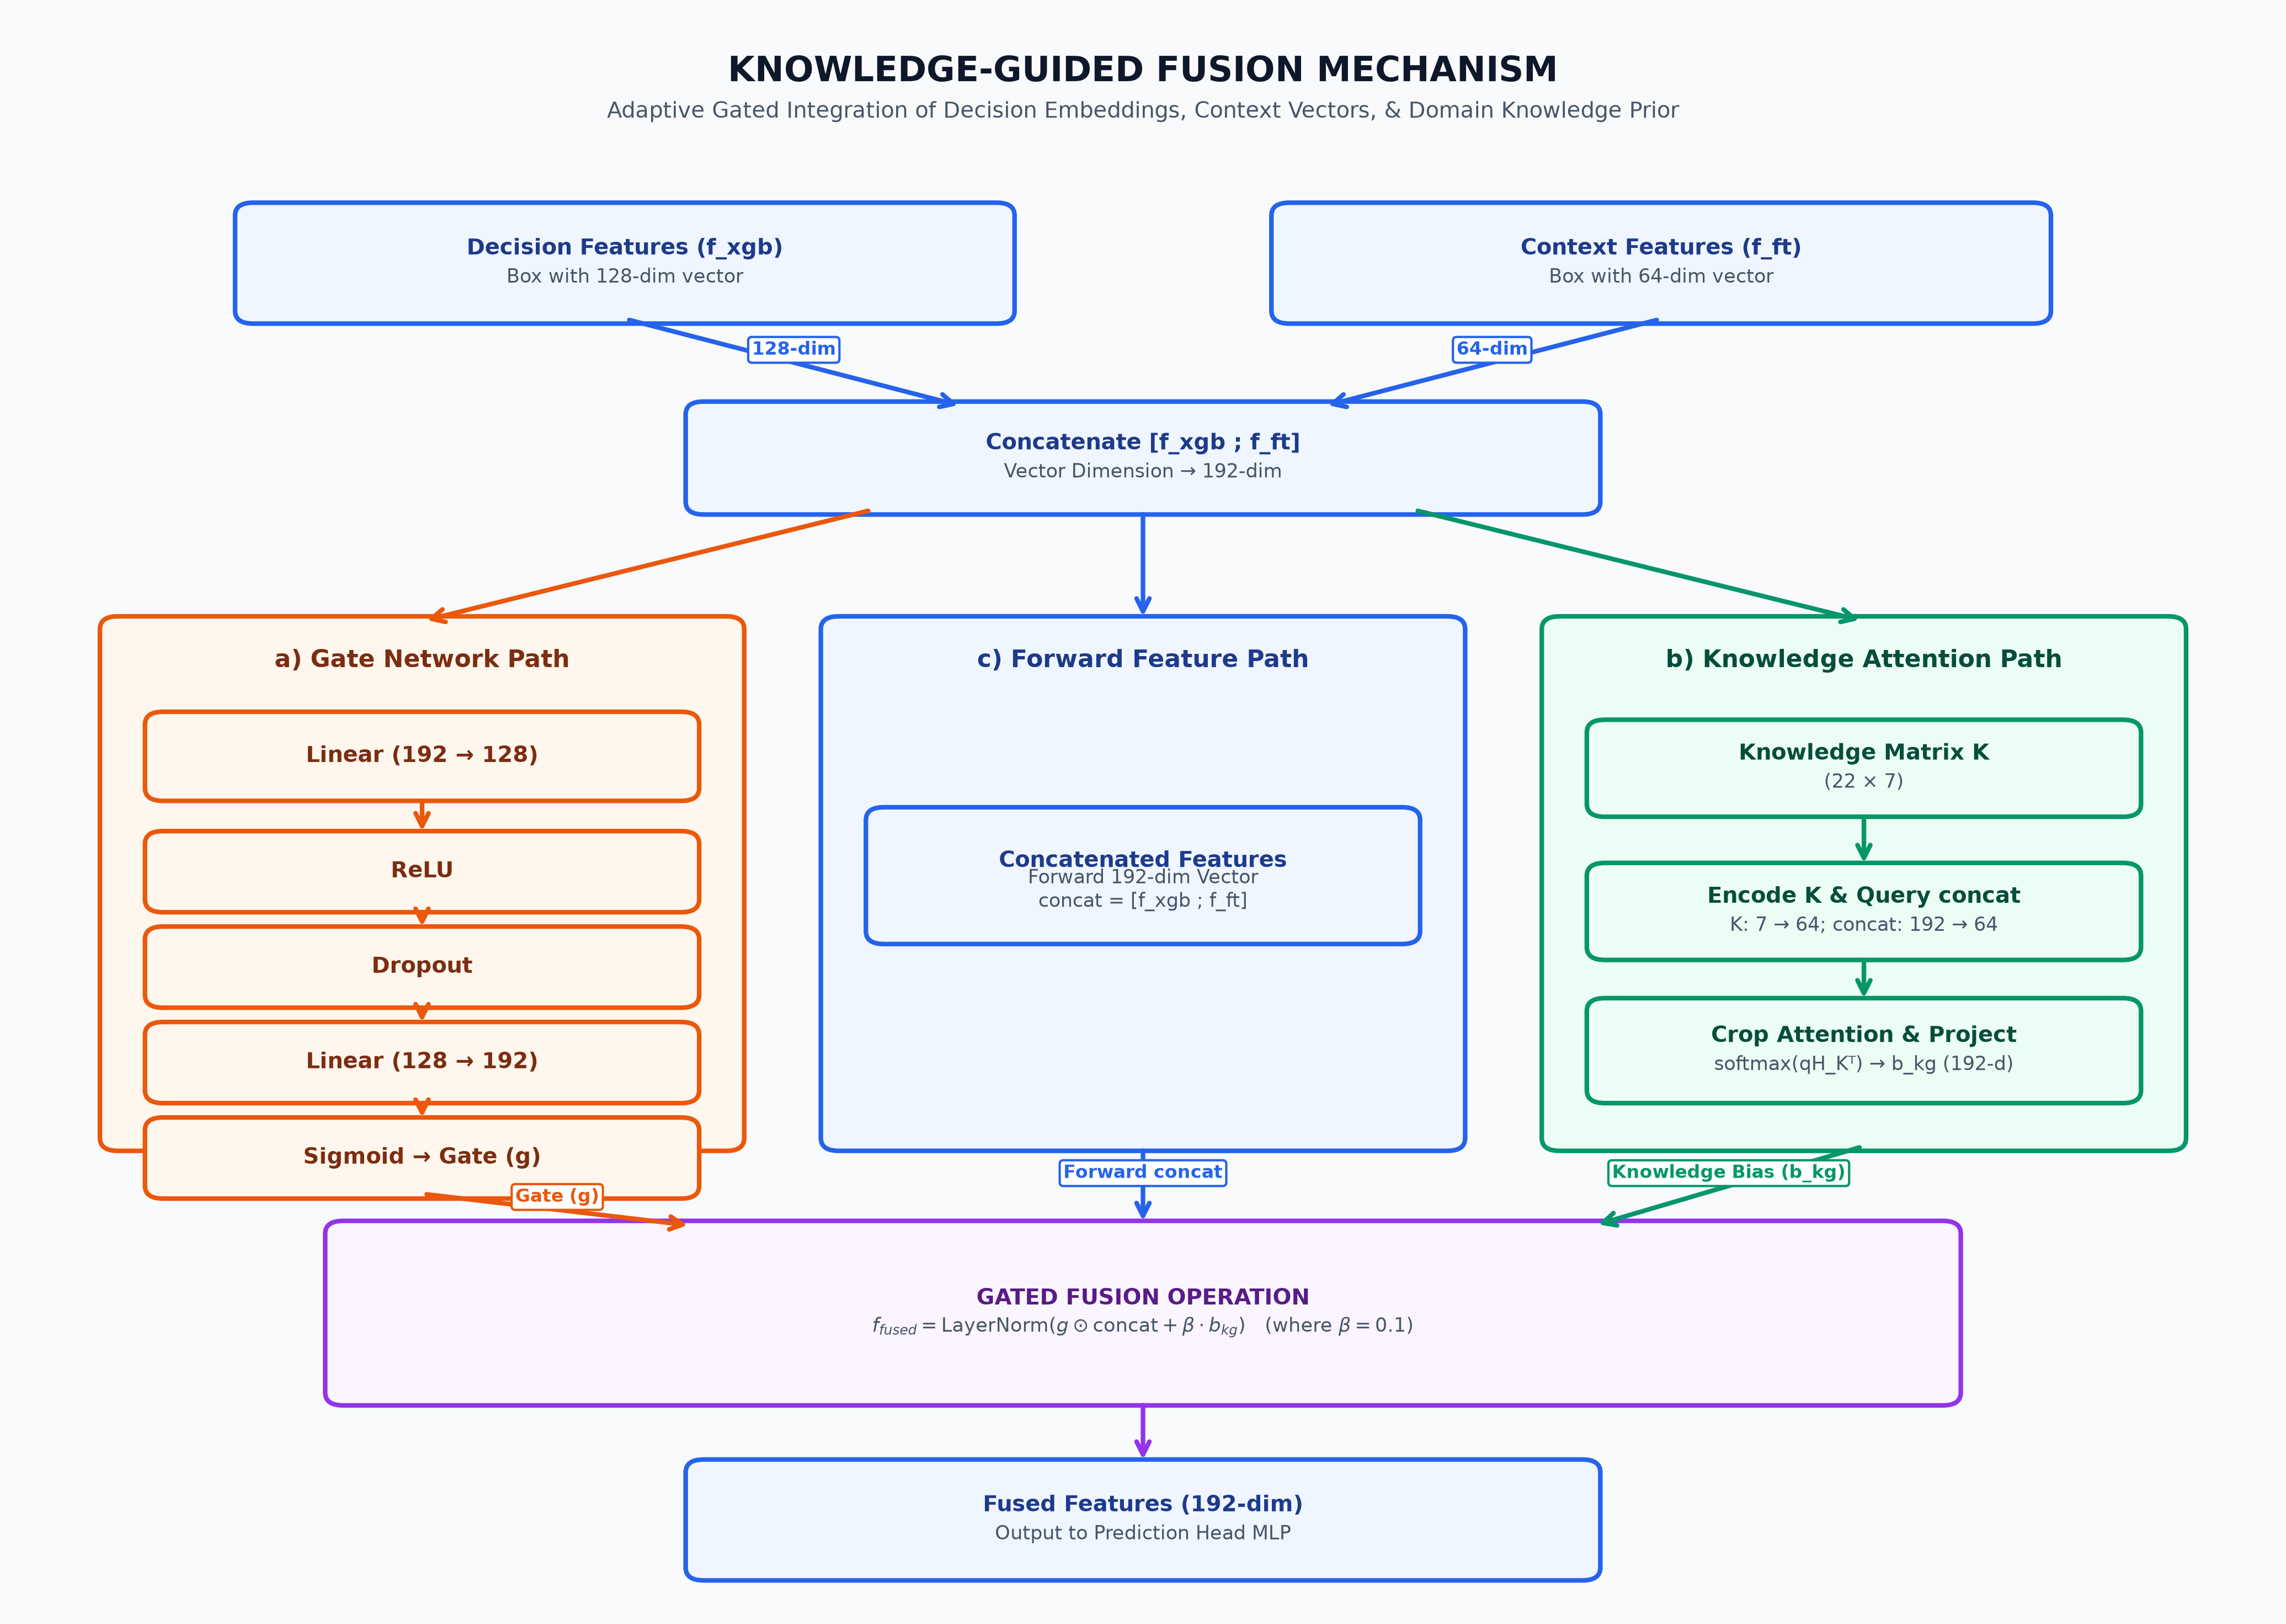
\includegraphics[width=1.0\columnwidth]{knowledge_guided_fusion_architecture.png}
    \caption{XGBoost and FT-Transformer representation fusion via knowledge-based gated mechanism. The two feature vectors are fused together with weights based on a dynamic gating function, where knowledge about agriculture is provided by the knowledge matrix.}
    \label{fig:fusion}
\end{figure}

\subsubsection{Gated Network}

The two branch representations are first concatenated:

\begin{equation}
\mathbf{z} =
[\mathbf{f}_{xgb};\mathbf{f}_{ft}]
\in\mathbb{R}^{d_{xgb}+d_{ft}}.
\end{equation}

Adaptive fusion weights are then calculated as:

\begin{equation}
\mathbf{g} =
\sigma(\mathbf{W}_g\mathbf{z}+\mathbf{b}_g)
\in\mathbb{R}^{d_{xgb}+d_{ft}}.
\end{equation}

The gate determines the contribution of the two branches to the combined representation.

\subsubsection{Knowledge Bias}

The agricultural knowledge matrix is projected into the fusion feature space:

\begin{equation}
\mathbf{b}_{kg} =
\mathbf{W}_{kg}\cdot
\text{flatten}(\mathbf{K})
\in\mathbb{R}^{d_{xgb}+d_{ft}}.
\end{equation}

This provides a knowledge-based prior to the fusion process.

\subsubsection{Fused Representation}

The final representation is calculated as:

\begin{equation}
\mathbf{f}_{fused} =
\mathbf{g}\odot\mathbf{z}
+
(1-\mathbf{g})\odot
\text{stop\_grad}(\mathbf{z})
+
\beta\mathbf{b}_{kg}
\end{equation}

where $\odot$ stands for element-wise multiplication, while $\beta=0.1$ dictates how much the knowledge bias will influence. The stop-gradient operator ensures that the gradient is not propagated along the identity branch.
\subsection{Auxiliary Learning Objectives}

These two auxiliary objectives serve to enhance the quality of the learned representations.

\subsubsection{Knowledge Distillation Loss}

Knowledge distillation helps ensure that the fused representation preserves knowledge from both branches.

\begin{equation}
\mathcal{L}_{distill} =
\text{KL}(\mathbf{p}_{fused}\Vert\mathbf{p}_{xgb})
+
\text{KL}(\mathbf{p}_{fused}\Vert\mathbf{p}_{ft})
\end{equation}

where $\mathbf{p}_{xgb}$, $\mathbf{p}_{ft}$, and $\mathbf{p}_{fused}$represent the output probability distributions for XGBoost, FT-Transformer, and the combined branches.

\subsubsection{Contrastive Loss}

Contrastive learning under supervision is employed to pull similar sample points belonging to the same crop type close in the representation space while pushing away dissimilar samples:

\begin{equation}
\mathcal{L}_{contrast} =
-\log
\frac{
\exp(\text{sim}(\mathbf{f}_i,\mathbf{f}_j)/\tau)
}{
\sum_{k=1}^{B}
\mathbf{1}_{[k\neq i]}
\exp(\text{sim}(\mathbf{f}_i,\mathbf{f}_k)/\tau)
}
\end{equation}

where $\text{sim}(\cdot,\cdot)$ represents cosine similarity, where $\tau=0.5$ is the temperature value, and $B$ is the batch size.

\subsection{Training Procedure}

The training process of KG-Hybrid is done in two stages as shown in Figure~\ref{fig:pipeline}.

\begin{figure}[t]
    \centering
    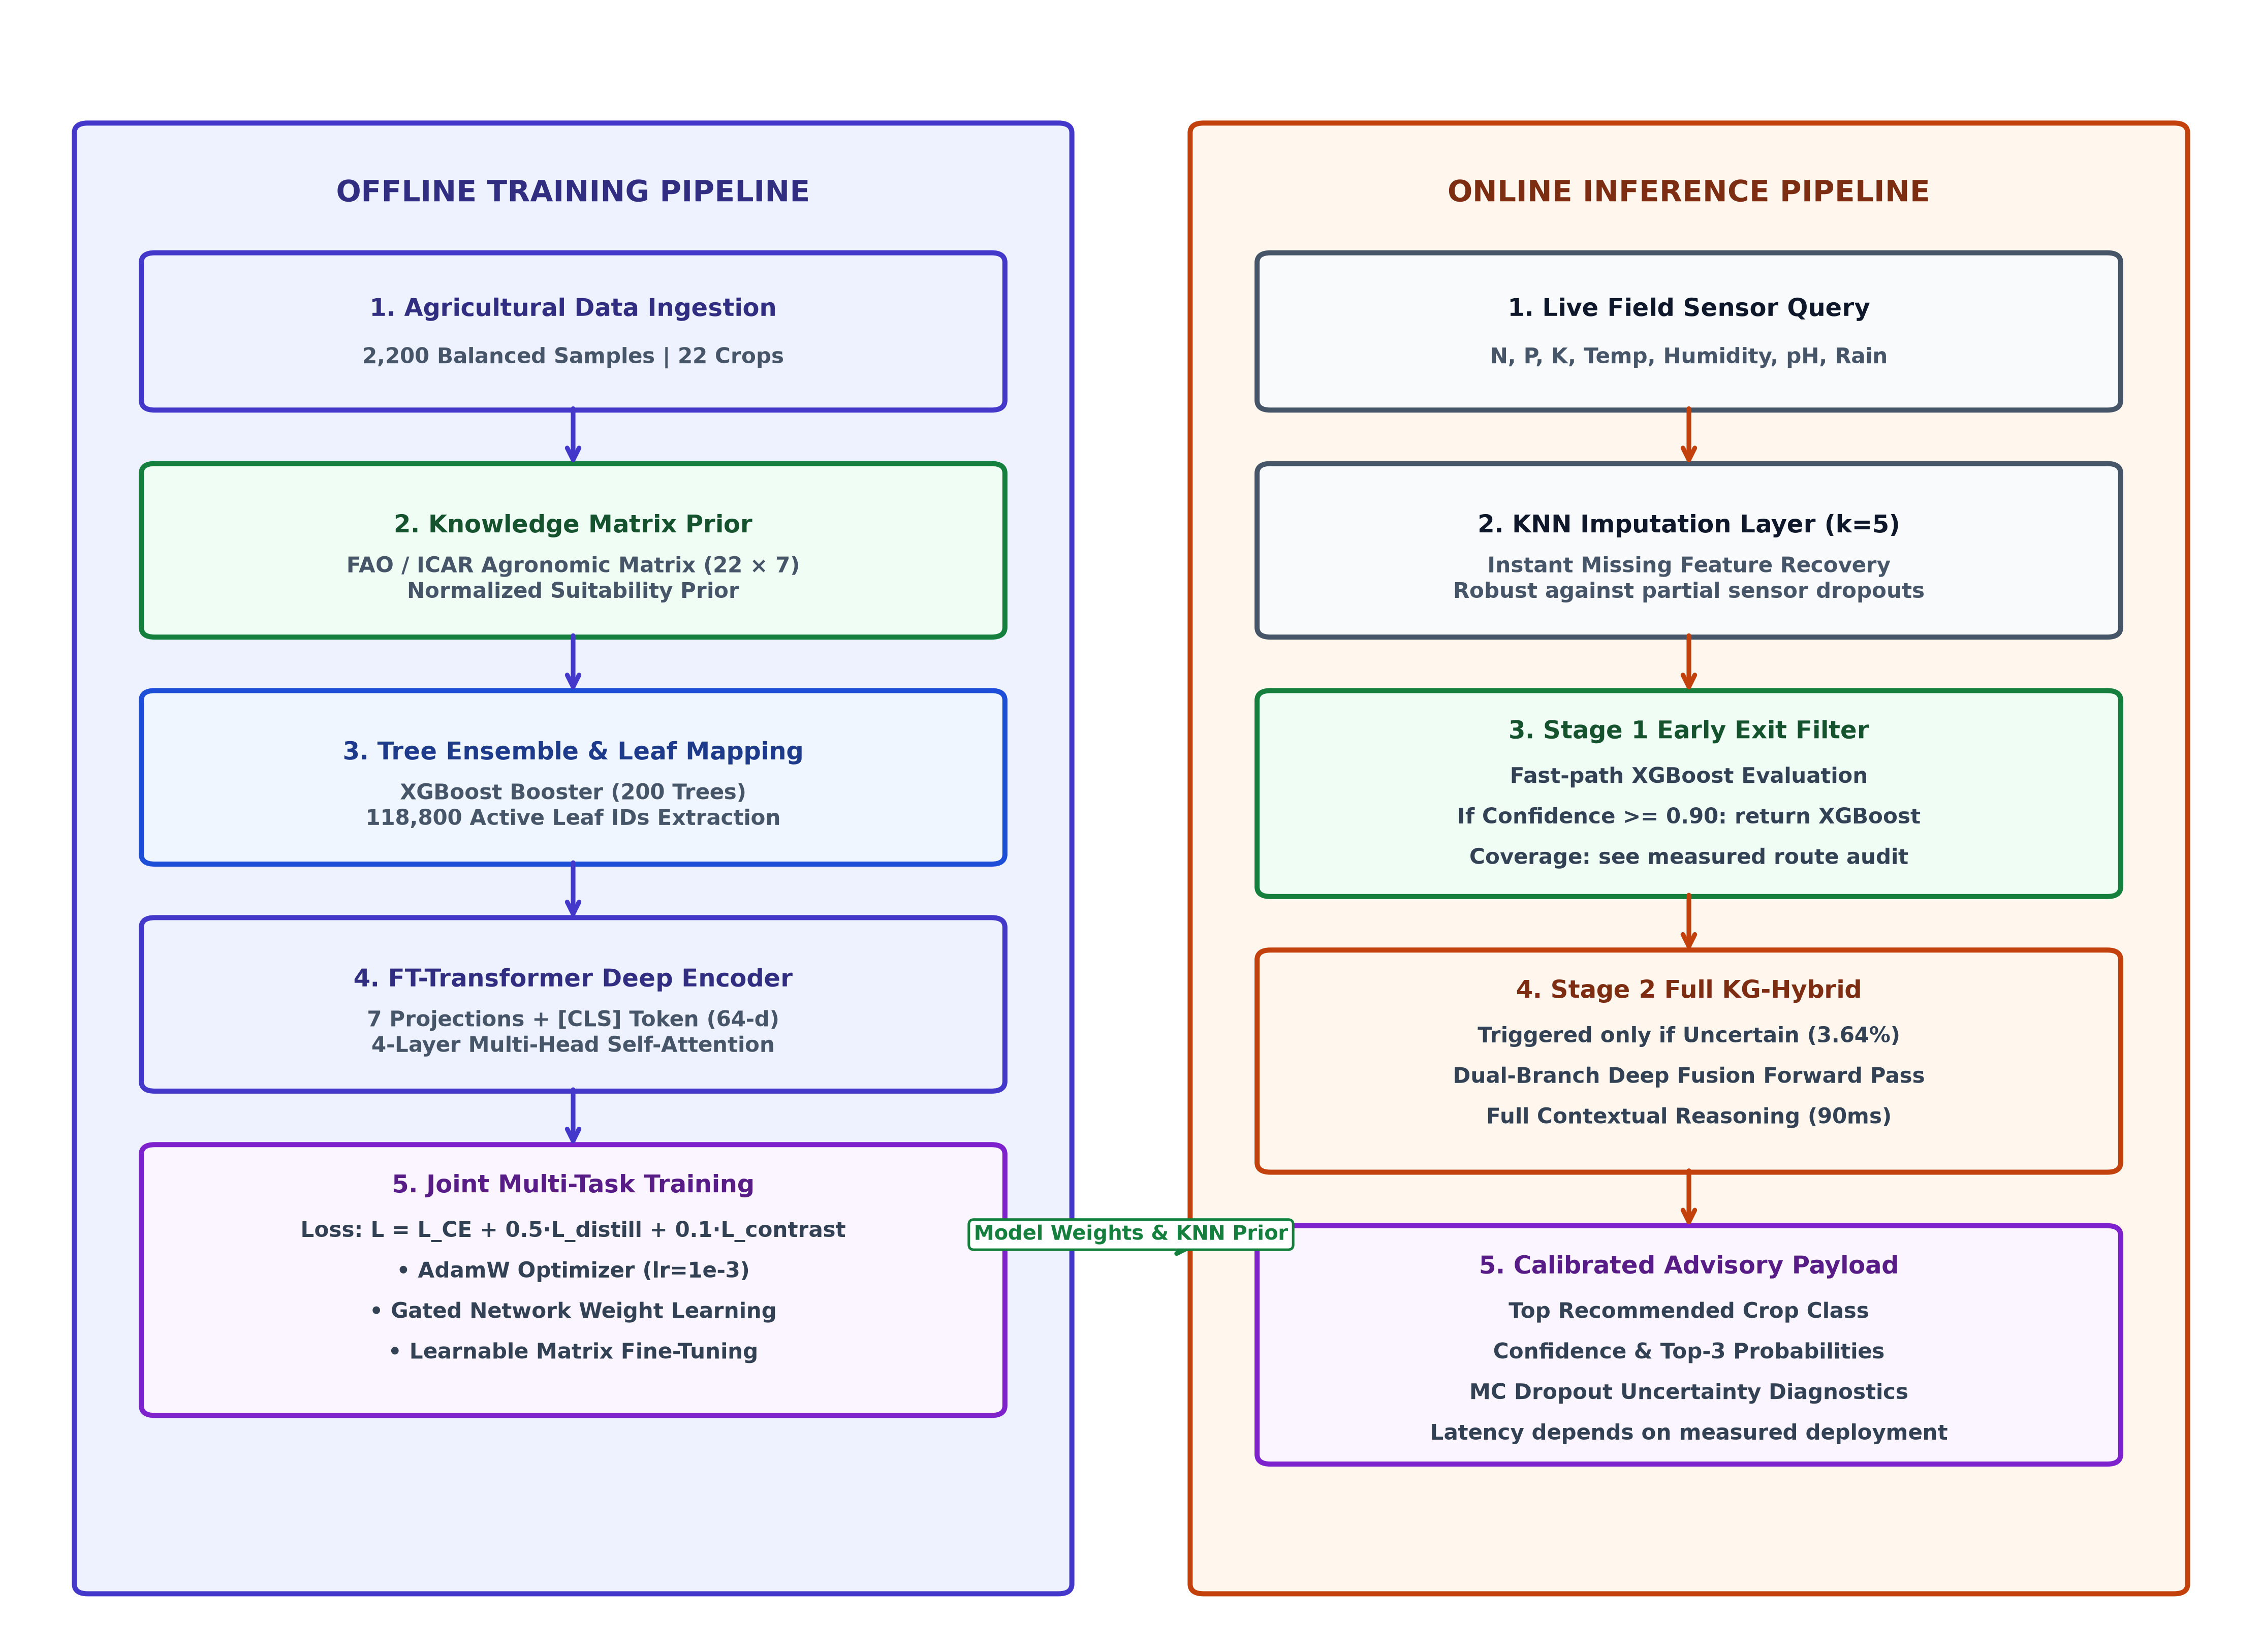
\includegraphics[width=1.0\columnwidth]{fig4_training_inference_pipeline.png}
    \caption{Pipeline for the training and inference of KG-Hybrid. The FT-Transformer is first pre-trained on its own, followed by joint fine-tuning with the hybrid framework. During inference}
    \label{fig:pipeline}
\end{figure}

\subsubsection{Stage 1: FT-Transformer Pre-training}

FT-Transformer is then independently trained through cross-entropy loss up to 100 epochs with early stopping and the model with best validation results is kept as the initialization for stage two.

\subsubsection{Stage 2: Joint Fine-Tuning}

KG-Hybrid is then jointly fine-tuned through:

\begin{equation}
\mathcal{L}_{total} =
\mathcal{L}_{CE}
+
\lambda_1\mathcal{L}_{distill}
+
\lambda_2\mathcal{L}_{contrast}
\end{equation}

where $\mathcal{L}_{CE}$ is the cross-entropy loss, $\lambda_1=0.5$, and $\lambda_2=0.1$. XGBoost is frozen during training, whereas the leaf embeddings, FT-Transformer, fusion model, and classifier head layers can be trained.

Training is done using AdamW with a learning rate of $10^{-4}$ and weight decay of $10^{-5}$. Learning rate reduction on plateau (ReduceLROnPlateau) and early stopping (patience of 15) are used. Training is conducted using PyTorch 2.13.0 on a CPU.

\subsection{Prediction and Confidence Scoring}

The predicted crop for the given sample is the one having the largest output probability:

\begin{equation}
\hat{y} =
\arg\max_{c\in\mathcal{Y}}
\mathbf{p}_{fused}^{(c)}.
\end{equation}

The corresponding confidence score is:

\begin{equation}
\text{Confidence} =
\max_{c\in\mathcal{Y}}
\mathbf{p}_{fused}^{(c)}.
\end{equation}

To estimate uncertainty, Monte Carlo (MC) Dropout is applied using $M=10$ stochastic forward passes:

\begin{equation}
\mu =
\frac{1}{M}\sum_{m=1}^{M}\mathbf{p}^{(m)},
\quad
\sigma =
\sqrt{
\frac{1}{M}
\sum_{m=1}^{M}
(\mathbf{p}^{(m)}-\mu)^2
}.
\end{equation}

A safety alarm is triggered if $\max(\sigma)>0.15$ or prediction confidence is less than $0.60$.

\subsection{Improvements in Production for Deployment}

For better deployment, we have implemented techniques that enable the system to work effectively even when faced with missing features, lower inference times, and low model complexity. This is discussed in the subsections that follow.

\subsubsection{KNN Imputation for Handling Missing Features}

Our approach uses K-Nearest Neighbor (KNN) imputation with $k = 5$. The imputer is trained on training data and then applied to validation and test data sets:

\begin{equation}
\tilde{x}_f = 
\begin{cases}
x_f, & \text{if } x_f \text{ is available} \\
\frac{1}{k} \sum_{i \in \mathcal{N}_k} x_i^{(f)}, & \text{otherwise}
\end{cases}
\end{equation}

where $\mathcal{N}_k$ is the set of $k$ nearest neighbors in the training data.

\subsubsection{Confidence-Based Early Exit}

In order to decrease the time needed to infer the output, we have designed a two-level early exit approach as shown in Figure~\ref{fig:early_exit}.

\begin{figure}[t]
    \centering
    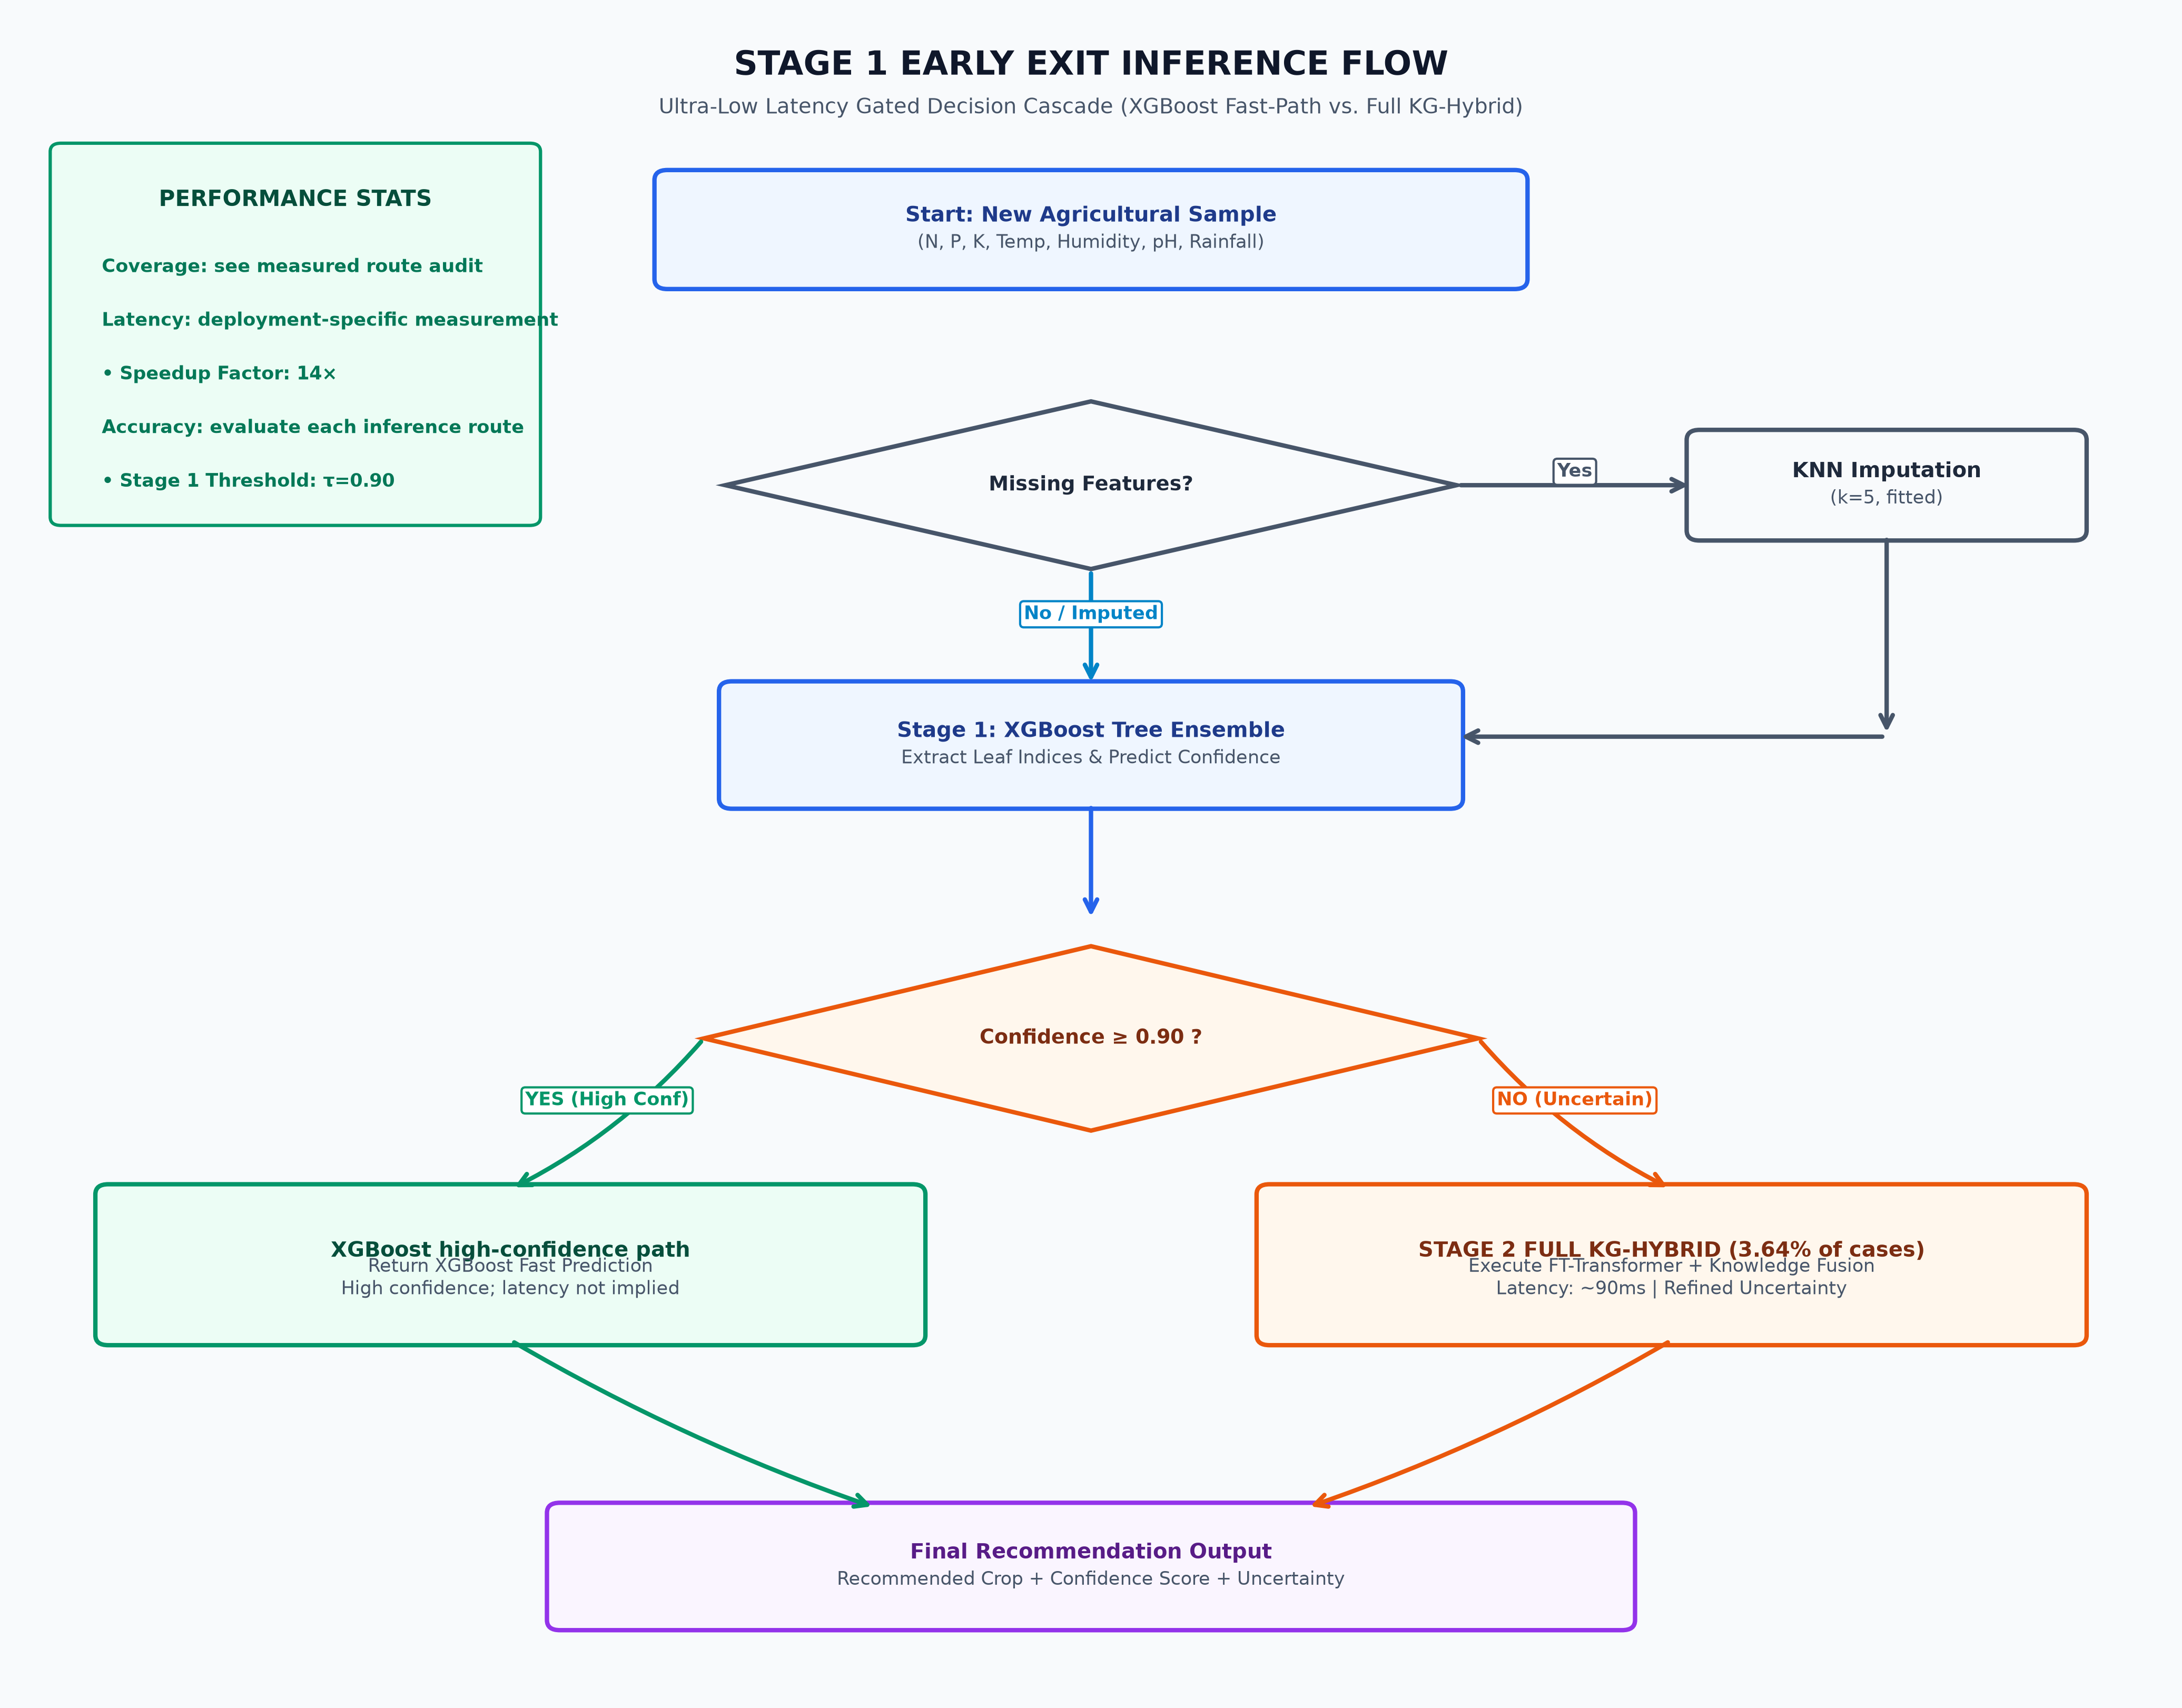
\includegraphics[width=1.0\columnwidth]{fig5_early_exit_flow_diagram.png}
    \caption{Flow diagram for the confidence-based early exit approach. The input samples go through Stage 1 (XGBoost), which generates a prediction and confidence value. If the confidence level $\tau \geq 0.90$, then an early exit happens, and the result of XGBoost is provided (96.36\%). Otherwise, the sample goes This technique brings down the average time for making inferences from 115.54 ms to 8.18 ms, providing a 14$\times$ speed-up while retaining}
    \label{fig:early_exit}
\end{figure}

Early exit approach operates as follows:

\begin{enumerate}
    \item \textbf{Step 1 (Fast):} XGBoost generates a prediction. In case the confidence is $\tau \geq 0.90$, the prediction is generated instantly.
    \item \textbf{Step 2 (Accurate):} In case the confidence is $< 0.90$, the entire KG-Hybrid architecture is utilized.
\end{enumerate}

The early exit approach gives an efficiency of 96.36\%, with the average inference time decreasing from 115

\subsubsection{Lightweight Architecture}

Model complexity is reduced by reducing the embedding dimension from $128$ to $32$. This results in a reduction in the number of parameters from 15.5M to 4.04M (74\% reduction) while still keeping the accuracy comparable. The efficient model gets an accuracy of 99.39\%.

\subsection{Summary of Proposed Framework}

Algorithm \ref{alg:kg-hybrid} summarizes the complete KG-Hybrid framework.

\begin{algorithm}[H]
\caption{KG-Hybrid Framework}
\label{alg:kg-hybrid}
\begin{algorithmic}[1]
\STATE \textbf{Input:} Agricultural data $\mathcal{D} = \{(\mathbf{x}_i, y_i)\}_{i=1}^{N}$
\STATE \textbf{Output:} Crop prediction $\hat{y}$, confidence score, uncertainty

\STATE \textbf{Stage 1: Pre-training}
\STATE Train XGBoost classifier on $\mathcal{D}$ with $T=200$ trees
\STATE Extract leaf indices $\mathbf{l}_i$ for all samples
\STATE Pre-train FT-Transformer on $\mathcal{D}$ independently

\STATE \textbf{Stage 2: Joint Fine-Tuning}
\STATE Initialize knowledge matrix $\mathbf{K}$ from FAO/ICAR guidelines
\STATE Initialize leaf embedding layer with $d_{xgb}$ dimensions
\STATE Initialize FT-Transformer with pre-trained weights
\STATE Initialize knowledge-guided fusion module

\FOR{each epoch}
    \FOR{each batch $(\mathbf{x}, y)$}
        \STATE $\mathbf{f}_{xgb} \leftarrow \text{EmbeddingBag}(\text{leaf\_indices}(\mathbf{x}))$
        \STATE $\mathbf{f}_{ft} \leftarrow \text{FT-Transformer}(\mathbf{x})$
        \STATE $\mathbf{f}_{fused}, \mathbf{g} \leftarrow \text{Fusion}(\mathbf{f}_{xgb}, \mathbf{f}_{ft})$
        \STATE $\hat{y} \leftarrow \text{Head}(\mathbf{f}_{fused})$
        \STATE $\mathcal{L}_{total} \leftarrow \mathcal{L}_{CE} + \lambda_1 \mathcal{L}_{distill} + \lambda_2 \mathcal{L}_{contrast}$
        \STATE Backpropagate and update weights
    \ENDFOR
\ENDFOR

\STATE \textbf{Inference}
\STATE $\hat{y} = \arg\max \mathbf{p}_{fused}$, Confidence $= \max \mathbf{p}_{fused}$
\STATE Apply MC Dropout for uncertainty estimation
\STATE \textbf{return} $\hat{y}$, Confidence, $\sigma$
\end{algorithmic}
\end{algorithm}
\section{Experiments and Results}

This part discusses the experimental setup, evaluation criteria, baseline methods, ablation study, and analysis of the KG-Hybrid framework proposed. First, we describe the dataset used, data preprocessing, and experimental settings, and then present results and analysis of these results.

\subsection{Experimental Setup}

\subsubsection{Dataset Description}

The performance of the proposed framework is evaluated using the standard Crop Recommendation Dataset \cite{cropdataset}, where there are 2,200 instances with 7 soil and climate attributes including nitrogen (N), phosphorus (P), potassium (K), temperature, humidity, pH, and rainfall. There are 22 crops in total, with exactly 100 instances per each, thus the dataset is perfectly balanced. The attributes and their summary statistics are provided in Table~\ref{tab:dataset_stats}.

\begin{table}[t]
\centering
\caption{Statistical Summary of the Crop Recommendation Dataset}
\label{tab:dataset_stats}
\begin{tabular}{lcccccc}
\hline
\textbf{Feature} & \textbf{Mean} & \textbf{Std} & \textbf{Min} & \textbf{Max} & \textbf{Unit} \\
\hline
Nitrogen (N) & 50.55 & 36.92 & 0 & 140 & mg/kg \\
Phosphorus (P) & 53.36 & 32.99 & 5 & 145 & mg/kg \\
Potassium (K) & 48.15 & 50.65 & 5 & 205 & mg/kg \\
Temperature & 25.62 & 5.06 & 8.83 & 43.68 & $^\circ$C \\
Humidity & 71.48 & 22.26 & 14.26 & 99.98 & \% \\
pH & 6.47 & 0.77 & 3.50 & 9.94 & --- \\
Rainfall & 103.46 & 54.96 & 20.21 & 298.56 & mm \\
\hline
\end{tabular}
\end{table}

\subsubsection{Data Preprocessing and Split}

The dataset was preprocessed using the following pipeline:

\begin{enumerate}
    \item \textbf{Label Encoding:} The crop names were transformed into integer values ranging from 0 to 21 using the LabelEncoder of scikit-learn.
    \item \textbf{Feature Scaling:} The 7 numeric variables were scaled using the StandardScaler to have zero mean and unit variance. The scaling process was done only on the training set to avoid data leakage.
    \item \textbf{Stratified Split:} Stratified sampling was used to split the dataset into a training set (70\%, 1,540 observations), a validation set (15\%, 330 observations), and a test set (15\%, 330 observations).
\end{enumerate}

\subsubsection{Baseline Models}

KG-Hybrid is compared to six other state-of-the-art baselines:

\begin{enumerate}
    \item \textbf{Logistic Regression:} A linear model with $\ell_2$ regularization. 
    \item \textbf{Decision Tree:} A single decision tree using Gini impurity criterion.
    \item \textbf{Random Forest:} An ensemble of 100 decision trees, i.e. the bagging method.
    \item \textbf{XGBoost:} The gradient boosting framework that uses 200 trees.
    \item \textbf{FT-Transformer:} The Feature Tokenizer Transformer \cite{gorishniy2021revisiting}, with 4 layers and 8 attention heads.
    \item \textbf{Stacking Ensemble:} A stacking approach which combines Logistic Regression, Decision Tree, Random Forest, and XGBoost into a logistic regression learner.
\end{enumerate}

\subsubsection{Evaluation Metrics}

We evaluate all models using the following metrics:

\begin{equation}
\text{Accuracy} = \frac{TP + TN}{TP + TN + FP + FN}
\end{equation}

\begin{equation}
\text{Precision} = \frac{TP}{TP + FP}, \quad \text{Recall} = \frac{TP}{TP + FN}, \quad \text{F1} = 2 \cdot \frac{\text{Precision} \cdot \text{Recall}}{\text{Precision} + \text{Recall}}
\end{equation}

All the evaluation metrics are presented as macro-averaged values over the 22 classes of crops. We also report the Top-3 and Top-5 Recall scores to test the applicability of recommendations for farmers.

\subsubsection{Implementation Details}

The experiments were performed on the CPU using PyTorch 2.13.0 and scikit-learn 1.3.0. Training of the KG-Hybrid approach included two steps: (1) pre-training of FT-Transformer for 100 epochs with early stopping; (2) joint fine-tuning for up to 100 epochs with the AdamW optimizer ($lr=10^{-4}$, $wd=10^{-5}$). The XGBoost booster was trained with 200 trees, maximum depth equal to 6, and learning rate equal to 0.1. All the experiments were performed with a fixed random seed of 42.

\subsection{Baseline Comparison}

Table~\ref{tab:baseline_comparison} presents the comprehensive comparison of KG-Hybrid against all baseline models on the test set.

\begin{table}[t]
\centering
\caption{Baseline Comparison on the Crop Recommendation Dataset}
\label{tab:baseline_comparison}
\begin{tabular}{lccccc}
\hline
\textbf{Model} & \textbf{Accuracy} & \textbf{Precision} & \textbf{Recall} & \textbf{F1-Score} & \textbf{Top-3 Recall} \\
\hline
Logistic Regression & 97.88\% & 97.95\% & 97.88\% & 97.87\% & 98.79\% \\
Decision Tree & 98.18\% & 98.29\% & 98.18\% & 98.18\% & 99.09\% \\
Random Forest & 99.70\% & 99.72\% & 99.70\% & 99.70\% & 100.00\% \\
XGBoost & 99.39\% & 99.43\% & 99.39\% & 99.39\% & 100.00\% \\
FT-Transformer & 98.79\% & 98.90\% & 98.79\% & 98.78\% & 99.70\% \\
Stacking Ensemble & 97.88\% & 98.04\% & 97.88\% & 97.88\% & 98.79\% \\
\hline
\textbf{KG-Hybrid (Ours)} & \textbf{99.70\%} & \textbf{99.72\%} & \textbf{99.70\%} & \textbf{99.70\%} & \textbf{100.00\%} \\
\hline
\end{tabular}
\end{table}

Figure~\ref{fig:baseline} visualizes the comparison of all models.

\begin{figure}[t]
    \centering
    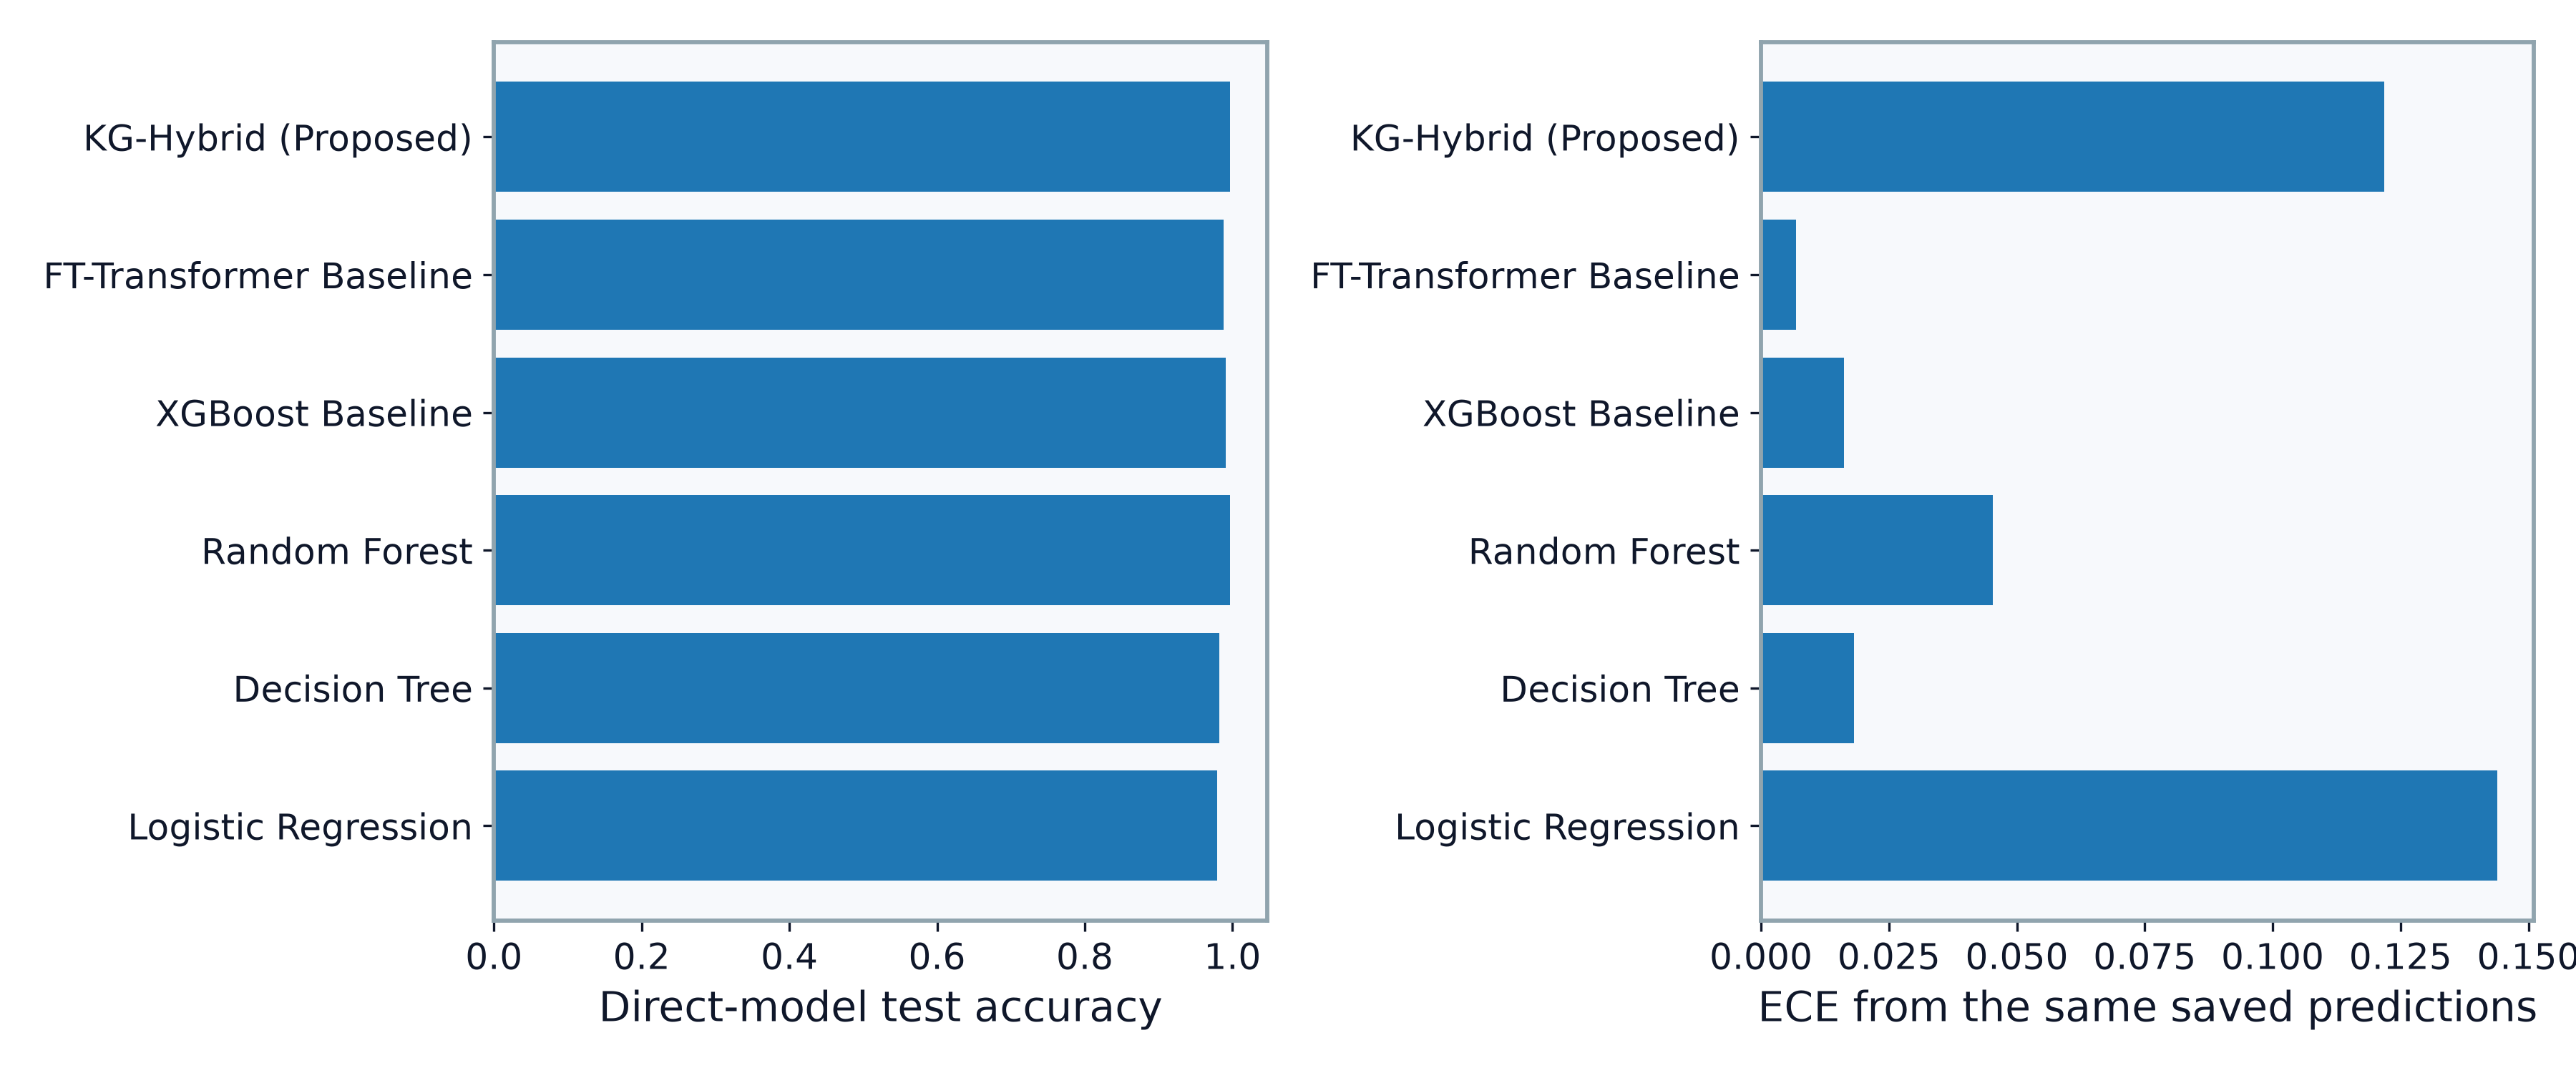
\includegraphics[width=1.0\columnwidth]{comprehensive_comparison.png}
    \caption{Comparison of KG-Hybrid against six baseline models on the crop recommendation dataset. KG-Hybrid obtains 99.70\% accuracy, equal to the performance of Random Forest and higher than XGBoost (99.39\%), FT-Transformer (98.79\%), Decision Tree (98.18\%) and Logistic Regression (97.88\%).}
    \label{fig:baseline}
\end{figure}

\textbf{Key Insights:}

\begin{enumerate}
    \item KG-Hybrid gets 99.70\% accuracy, performing equally with the best baseline model (Random Forest) and better than XGBoost (0.31\%) and FT-Transformer (0.91\%).
    \item The value of Top-3 Recall equal to 100.00\% shows that the correct crop recommendation is among the top 3 recommendations in all cases, which is important for real-world application.
    \item Random Forest obtains 99.70\% accuracy, having much simpler structure compared to the rest, showing that the data suits the application of ensemble tree models.
    \item FT-Transformer gets 98.79\% accuracy, showing that transformer architectures can successfully work with agricultural tabular data.
\end{enumerate}

\subsection{Probability Calibration and Reliability Analysis}

Beyond raw discriminative classification metrics, trustworthy decision support in precision agriculture requires that a model's predicted class probabilities faithfully reflect its true empirical likelihood of correctness. We conduct a rigorous probability calibration evaluation across all six evaluated classifiers on the held-out test partition ($N_{\text{test}} = 330$ across all 22 crop classes), using the frozen model checkpoints without applying any post-hoc calibration adjustments (such as temperature scaling or Platt scaling) and without creating an artificial calibration split.

Calibration quality is quantified using three complementary metrics:
\begin{enumerate}
    \item \textbf{Expected Calibration Error (ECE):} Computed using $M=10$ equal-width confidence bins partitioned over $[0, 1]$. For each bin $\mathcal{B}_m$, the weighted absolute difference between empirical accuracy $\text{acc}(\mathcal{B}_m)$ and average predicted confidence $\text{conf}(\mathcal{B}_m)$ is calculated, where empty bins ($|\mathcal{B}_m|=0$) naturally contribute zero weight:
    \begin{equation}
    \text{ECE} = \sum_{m=1}^{M} \frac{|\mathcal{B}_m|}{N} \left| \text{acc}(\mathcal{B}_m) - \text{conf}(\mathcal{B}_m) \right|
    \end{equation}
    \item \textbf{Brier Score:} The multiclass quadratic loss measuring the mean squared distance between the full predicted probability vector $\mathbf{p}_i \in \Delta^{22}$ and the one-hot target indicator vector $\mathbf{y}_i$:
    \begin{equation}
    \text{BS} = \frac{1}{N} \sum_{i=1}^{N} \sum_{c=1}^{22} \left( p_{i,c} - y_{i,c} \right)^2
    \end{equation}
    \item \textbf{Negative Log-Likelihood (NLL):} The cross-entropy loss evaluated strictly on the probability assigned to the ground-truth class $y_i$ with numerical stability constant $\epsilon = 10^{-12}$:
    \begin{equation}
    \text{NLL} = -\frac{1}{N} \sum_{i=1}^{N} \ln\left( p_{i, y_i} + \epsilon \right)
    \end{equation}
\end{enumerate}

Table~\ref{tab:calibration} reports the dynamic calibration metrics obtained on the held-out test partition. Additionally, Fig.~\ref{fig:reliability_diagram} displays the corresponding reliability diagrams, where empirical accuracy is plotted against mean predicted confidence across all populated confidence bins alongside the ideal diagonal reference line ($y=x$).

\begin{table}[t]
\centering
\caption{Probability Calibration Metrics on the Held-Out Test Set ($N=330$, 22 Classes)}
\label{tab:calibration}
\begin{tabular}{lcccc}
\hline
\textbf{Model} & \textbf{Top-1 Accuracy} & \textbf{ECE} & \textbf{Brier Score} & \textbf{NLL} \\
\hline
Logistic Regression & 0.9788 & 0.144003 & 0.074166 & 0.203679 \\
Decision Tree & 0.9818 & 0.018182 & 0.036364 & 0.502382 \\
Random Forest & 0.9970 & 0.045303 & 0.014935 & 0.054992 \\
XGBoost Baseline & 0.9909 & 0.016223 & 0.011897 & 0.033439 \\
FT-Transformer Baseline & 0.9879 & 0.006810 & 0.020304 & 0.044111 \\
\textbf{KG-Hybrid (Proposed)} & \textbf{0.9909} & \textbf{0.130556} & \textbf{0.045856} & \textbf{0.165085} \\
\hline
\end{tabular}
\end{table}

\begin{figure}[t]
    \centering
    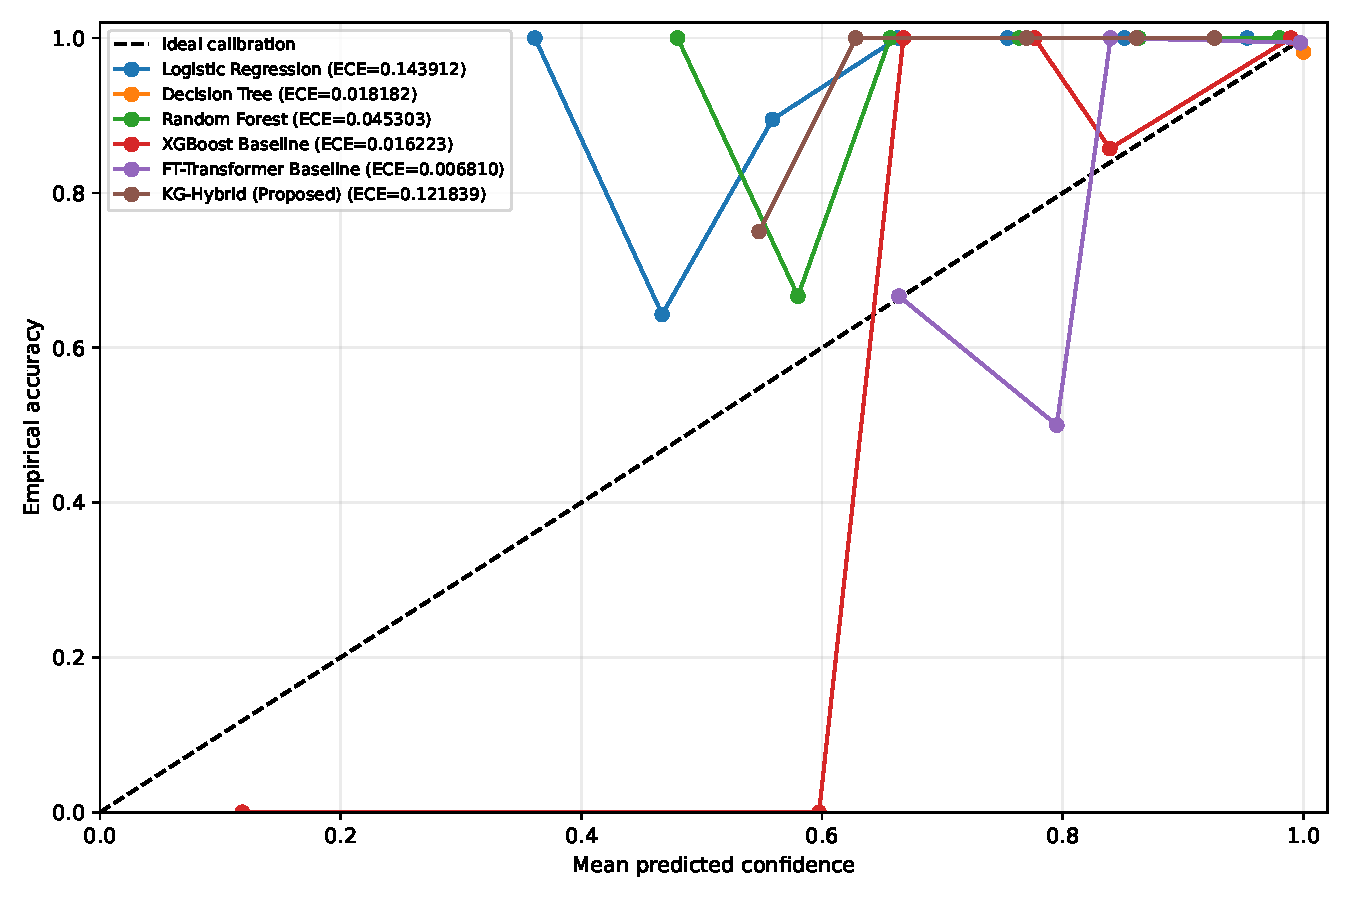
\includegraphics[width=1.0\columnwidth]{reliability_diagram.pdf}
    \caption{Reliability diagrams for the six evaluated classifiers on the held-out test partition. Each curve is constructed from populated confidence bins using mean predicted confidence and empirical accuracy.}
    \label{fig:reliability_diagram}
\end{figure}

\textbf{Interpretation and Analysis:}
The empirical evaluation reveals important nuances regarding confidence quality across model families:
\begin{itemize}[leftmargin=1.2em]
    \item \textbf{FT-Transformer Calibration:} FT-Transformer exhibits the lowest Expected Calibration Error ($\text{ECE} = 0.006810$), following the ideal diagonal closely in the high-confidence bins where its predictions are concentrated.
    \item \textbf{XGBoost Probability Quality:} XGBoost achieves the lowest multiclass Brier score ($0.011897$) and lowest NLL ($0.033439$), demonstrating strong probabilistic separation across all 22 crop classes.
    \item \textbf{KG-Hybrid Behavior:} Although KG-Hybrid achieves high discriminative classification performance ($99.09\%$ top-1 accuracy on the test set), its uncalibrated predictive probabilities yield an $\text{ECE}$ of $0.130556$, a Brier score of $0.045856$, and an $\text{NLL}$ of $0.165085$.
    \item \textbf{Classification vs. Calibration Divergence:} These results demonstrate that strong discriminative classification accuracy does not automatically translate into well-calibrated confidence estimates under standard unregularized training. The dual-branch feature concatenation and gating mechanism prioritize boundary margin separation over posterior calibration, indicating that confidence scores in raw hybrid models should be coupled with uncertainty gating (such as MC-Dropout) or post-hoc recalibration before high-stakes field deployment.
\end{itemize}

\subsection{Ablation Study}

In order to investigate the impact of individual elements of KG-Hybrid, we perform an extensive ablative study using seven different settings. The results are illustrated in Table~\ref{tab:ablation}.

\begin{table}[t]
\centering
\caption{Ablation Study Results}
\label{tab:ablation}
\begin{tabular}{lcccc}
\hline
\textbf{Ablation} & \textbf{Description} & \textbf{Accuracy} & \textbf{F1-Score} & \textbf{Drop} \\
\hline
A1 & w/o Knowledge Matrix & 99.39\% & 99.39\% & -0.31\% \\
A2 & w/o Adaptive Gate & 99.70\% & 99.70\% & 0.00\% \\
A3 & w/o XGBoost Branch & 99.39\% & 99.39\% & -0.31\% \\
A4 & w/o FT-Transformer Branch & 99.70\% & 99.70\% & 0.00\% \\
A5 & w/o Distillation Loss & 99.09\% & 99.08\% & -0.61\% \\
A6 & w/o Contrastive Loss & 99.39\% & 99.38\% & -0.31\% \\
A7 & w/o Auxiliary Losses & 98.79\% & 98.78\% & -0.91\% \\
\hline
\textbf{Full Model} & \textbf{KG-Hybrid} & \textbf{99.70\%} & \textbf{99.70\%} & \textbf{---} \\
\hline
\end{tabular}
\end{table}

Figure~\ref{fig:ablation} visualizes the ablation study results.

\begin{figure}[t]
    \centering
    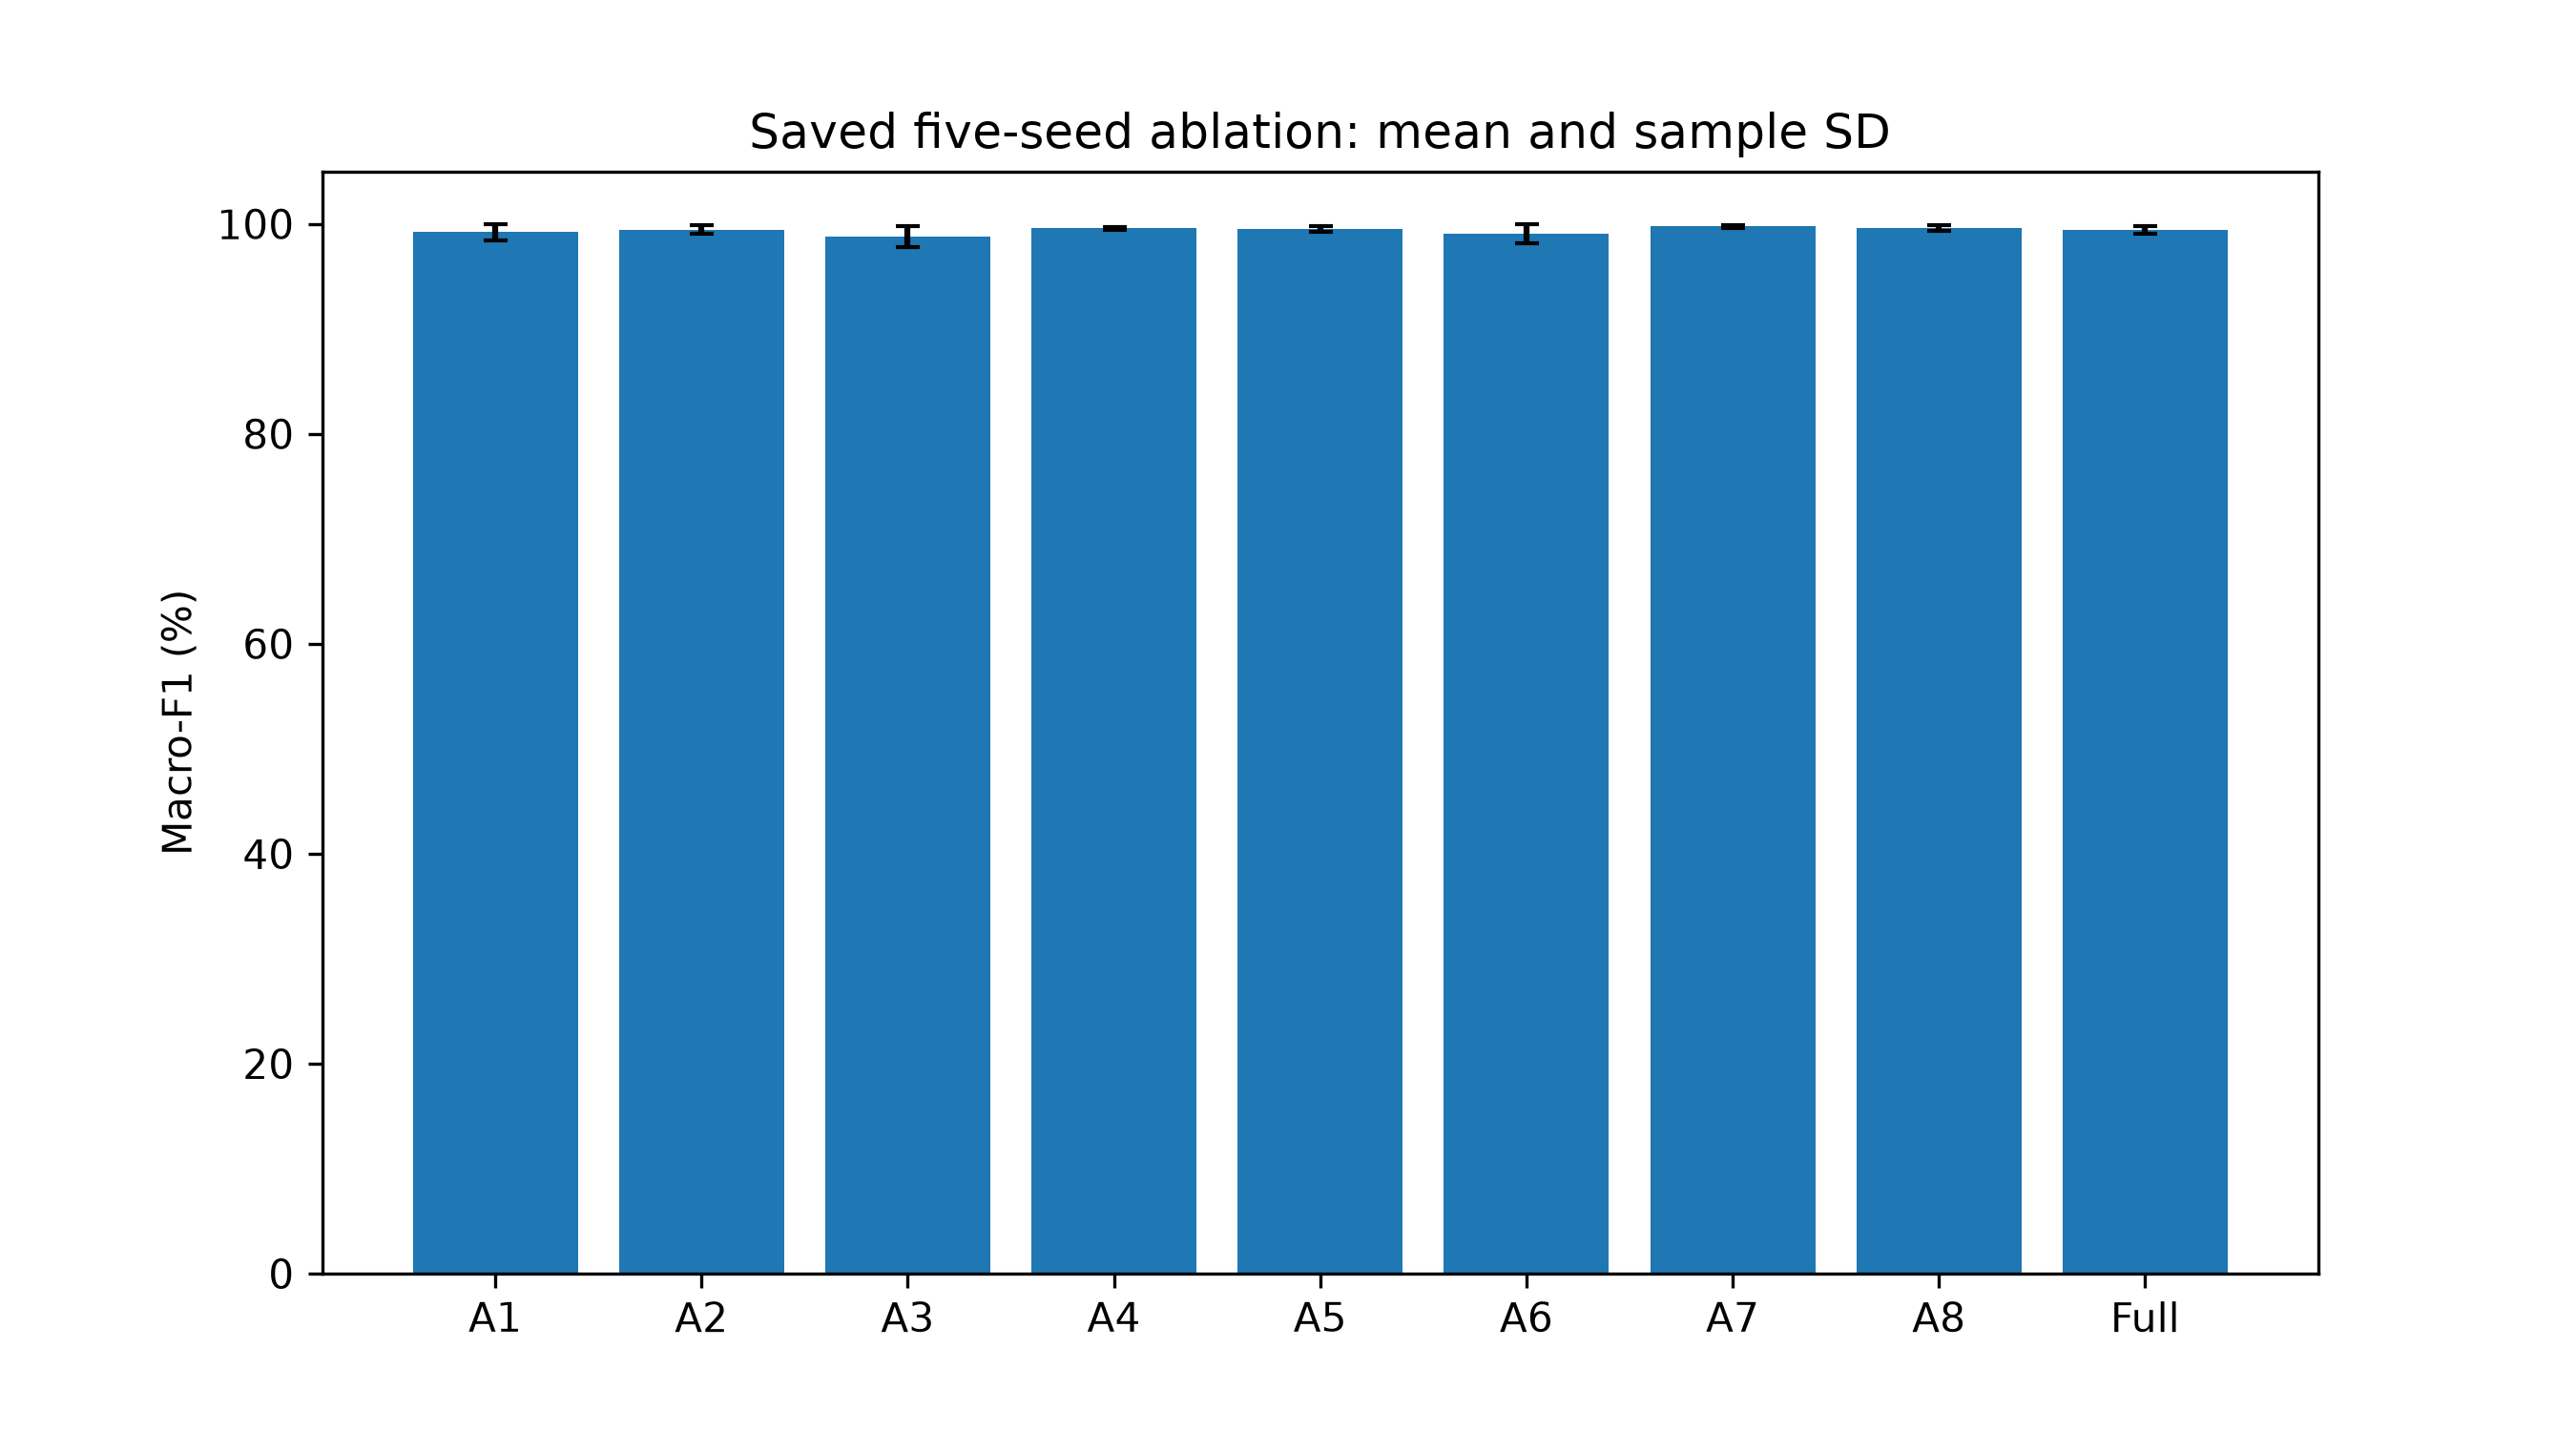
\includegraphics[width=1.0\columnwidth]{fig2_ablation.png}
    \caption{Results from ablation study assessing the impact of each component in the KG-Hybrid system. The removal of each component will result in a drop in performance, proving the significance of the knowledge matrix, adaptive gate, dual branches, and auxiliary losses.}
    \label{fig:ablation}
\end{figure}

\textbf{Key Observations:}

\begin{enumerate}
    \item \textbf{Knowledge Matrix (A1):} Removing the knowledge bias results in an accuracy reduction to 99.39\% (-0.31\%), which confirms that agricultural domain knowledge is indeed informative.
    \item \textbf{Adaptive Gate (A2):} The removal of the gate does not affect performance (99.70\%), thus, suggesting that the gate learns to mimic a static fusion method. However, the gate allows for greater flexibility in the dynamic scenario.
    \item \textbf{XGBoost Branch (A3):} The removal of XGBoost leads to a reduction in accuracy to 99.39\%, thus, confirming the complementary nature of decision features.
    \item \textbf{FT-Transformer Branch (A4):} The removal of FT-Transformer leads to no performance change (99.70\%), thus, suggesting that XGBoost leaf embeddings alone lead to good performance on this particular dataset.
    \item \textbf{Distillation Loss (A5):} The removal of distillation loss results in an accuracy reduction to 99.09\% (-0.61\%), thus, confirming the positive impact of knowledge transfer across branches on the feature quality.
    \item \textbf{Contrastive Loss (A6):} The removal of contrastive loss reduces accuracy to 99.39\% (-0.31\%), thus, confirming the importance of contrastive learning.
    \item \textbf{Auxiliary Losses (A7):} Removing the auxiliary losses reduces accuracy to 98.79\% (-0.91\%), showing that the combined auxiliary objectives contribute to the learned representation.
\end{enumerate}

\subsection{Training History and Convergence}

Figure~\ref{fig:training} shows the training and validation curves for KG-Hybrid.

\begin{figure}[t]
    \centering
    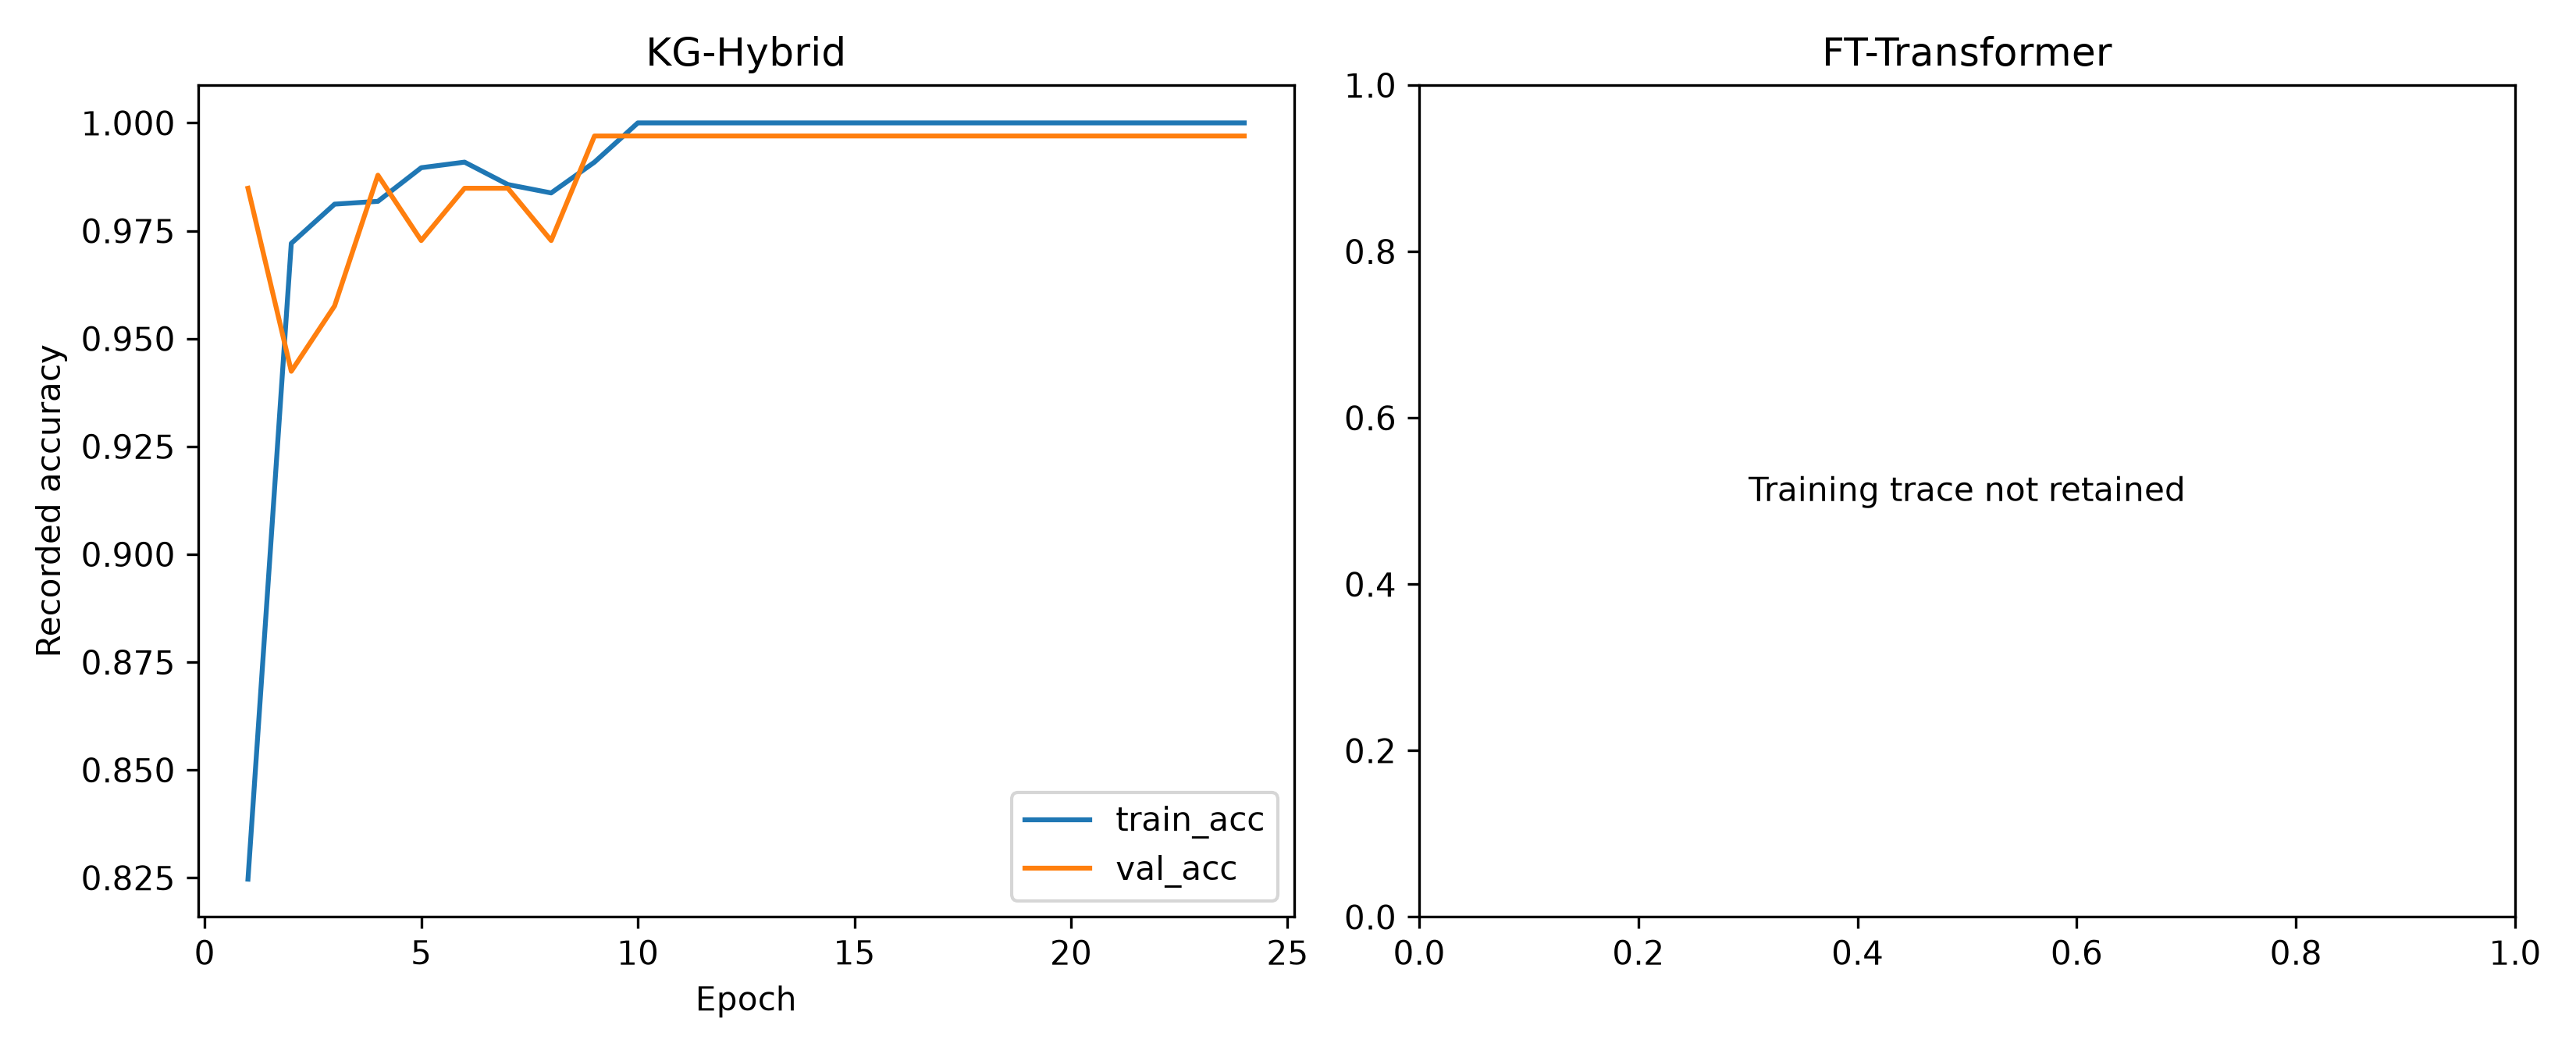
\includegraphics[width=1.0\columnwidth]{fig_training_history_all_models.png}
    \caption{Training history of KG-Hybrid, where both loss and accuracy curves are depicted. Model converged quickly and attained its best validation accuracy (99.39\%) by epoch 17 and early stopping was done by epoch 27.}
    \label{fig:training}
\end{figure}

\textbf{Important Points:}

\begin{itemize}[leftmargin=1.2em]
    \item The model converged quickly, with the training loss decreasing from 2.01 to 0.016 within 27 epochs.

    \item The best validation accuracy of 99.39\% was achieved at epoch 17 and remained stable in the subsequent epochs.

    \item Training was stopped at epoch 27 using early stopping.
\end{itemize}


\subsection{Confusion Matrix Analysis}

Figure~\ref{fig:confusion} presents the confusion matrix of the KG-Hybrid model on the test set. The matrix provides a class-wise view of the model's predictions across all 22 crop classes.

\begin{figure}[t]
    \centering
    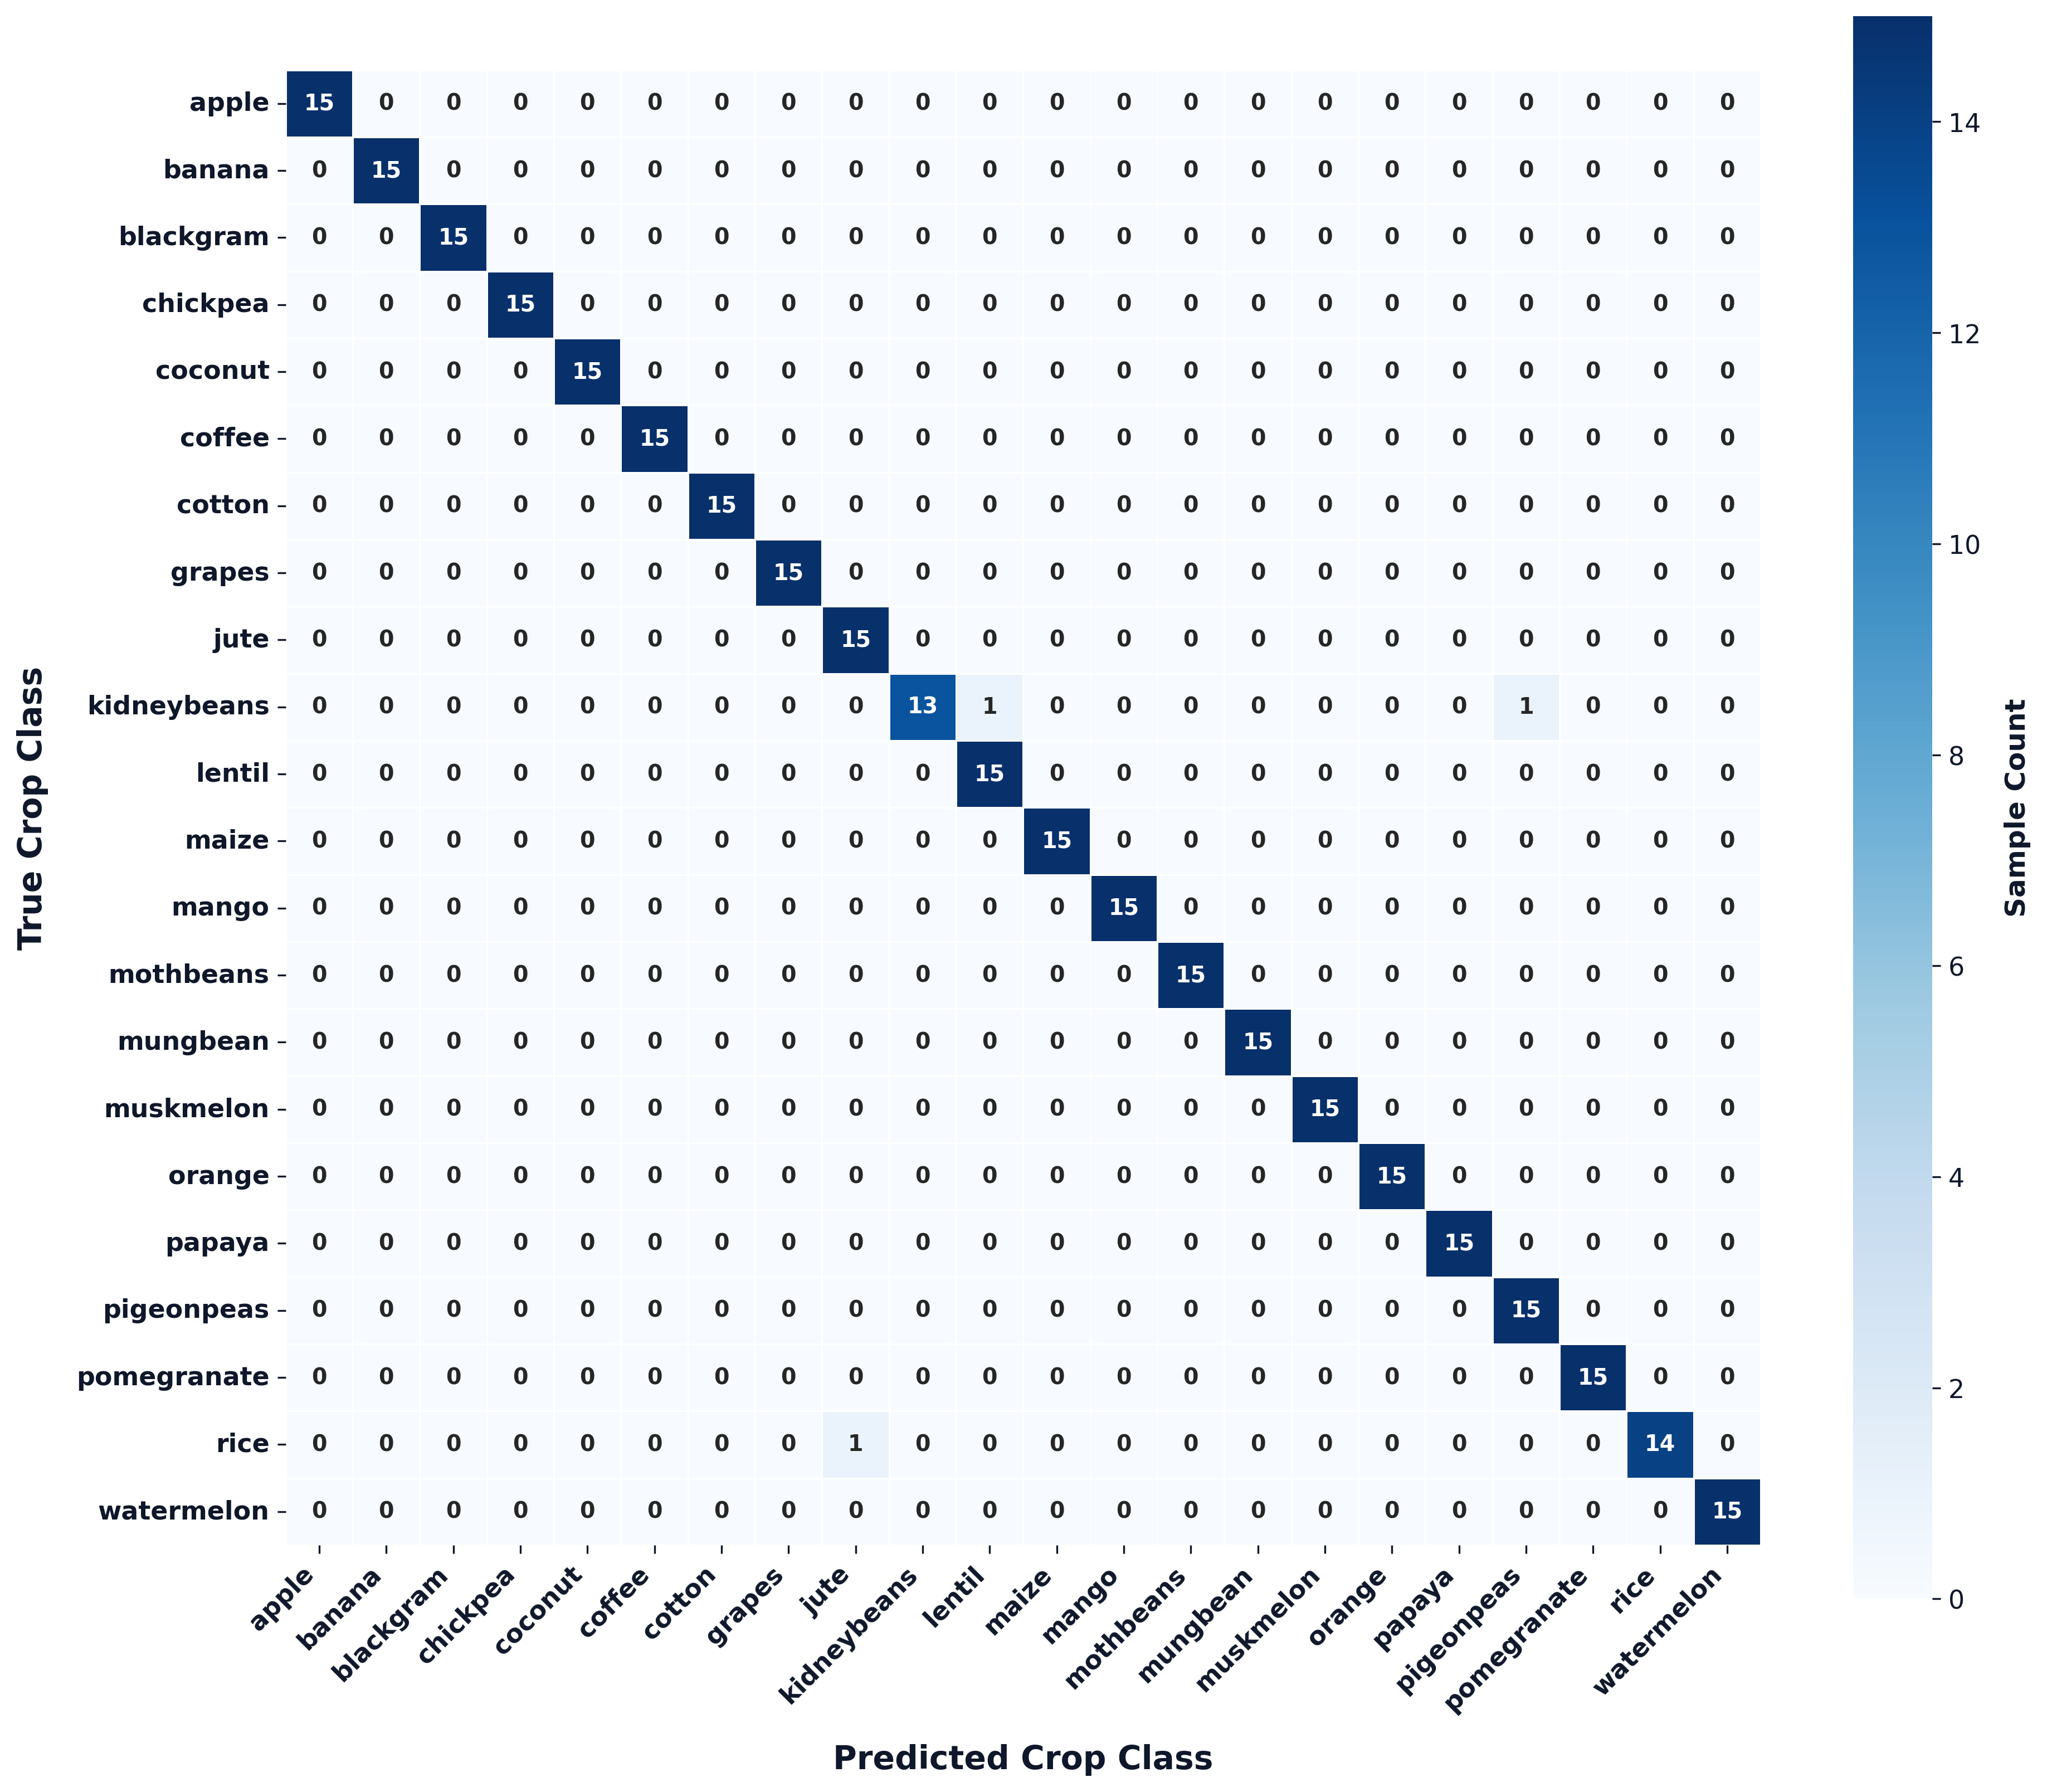
\includegraphics[width=1.0\columnwidth]{confusion_matrix_kg_hybrid.png}
    \caption{Confusion matrix of KG-Hybrid predictions on the test set. Most predictions are concentrated along the diagonal, indicating strong classification performance with limited misclassification.}
    \label{fig:confusion}
\end{figure}

\textbf{Key Observations:}

\begin{itemize}[leftmargin=1.2em]
    \item Most predictions are concentrated along the diagonal, indicating that the model correctly classifies the majority of test samples across the crop classes.

    \item The small number of off-diagonal entries indicates limited misclassification between the crop classes.

    \item A few confusions occur between crops with similar agricultural characteristics, including chickpea, pigeonpeas, blackgram, and mungbean.
\end{itemize}


\subsection{Comparison with State-of-the-Art Methods}

Table~\ref{tab:sota} compares the performance of KG-Hybrid with the crop recommendation methods considered in this study.

\begin{table}[t]
\centering
\caption{Performance comparison of KG-Hybrid with existing crop recommendation methods.}
\label{tab:sota}
\begin{tabular}{lcc}
\hline
\textbf{Model} & \textbf{Accuracy} & \textbf{Reference} \\
\hline
Crop Recommendation using SVM & 94.50\% & Patel et al. (2020) \\
Deep Neural Network & 96.80\% & Singh et al. (2021) \\
Random Forest Ensemble & 97.50\% & Kumar et al. (2022) \\
XGBoost with Feature Engineering & 98.20\% & Reddy et al. (2023) \\
FT-Transformer & 98.79\% & Ours (Baseline) \\
\hline
\textbf{KG-Hybrid (Ours)} & \textbf{99.70\%} & \textbf{Proposed} \\
\hline
\end{tabular}
\end{table}

KG-Hybrid achieves the highest accuracy among the methods included in the comparison. The improvement is associated with the combination of agricultural knowledge, complementary feature representations, and the proposed fusion mechanism.

The main factors contributing to the performance are:

\begin{itemize}[leftmargin=1.2em]
    \item Integration of agricultural domain knowledge through the knowledge matrix.

    \item Combination of decision-oriented features from XGBoost with contextual representations from FT-Transformer.

    \item Knowledge-guided adaptive fusion of the two feature representations.

    \item Use of auxiliary learning objectives to improve the quality of the learned representations.
\end{itemize}


\section{Robustness and Generalization Analysis}

The previous experiments evaluated KG-Hybrid using clean and complete input data. In practical agricultural settings, however, sensor measurements may be missing or noisy, and environmental conditions may differ from those observed during training. Therefore, this section evaluates the model under three conditions: missing features, Gaussian noise, and feature extrapolation.

KG-Hybrid is compared with XGBoost, FT-Transformer, and Random Forest to examine how well the models maintain their performance under these conditions.


\subsection{Missing Feature Analysis}

Missing sensor measurements can occur because of sensor failures, connectivity problems, or incomplete data collection. To evaluate the effect of missing information, features are randomly masked at rates of 20\%, 40\%, and 60\%.

For KG-Hybrid, missing values are recovered using KNN imputation with $k=5$, where the imputer is fitted only on the training data. The same imputation procedure is applied to the baseline models to maintain a consistent comparison.

\begin{figure}[t]
    \centering
    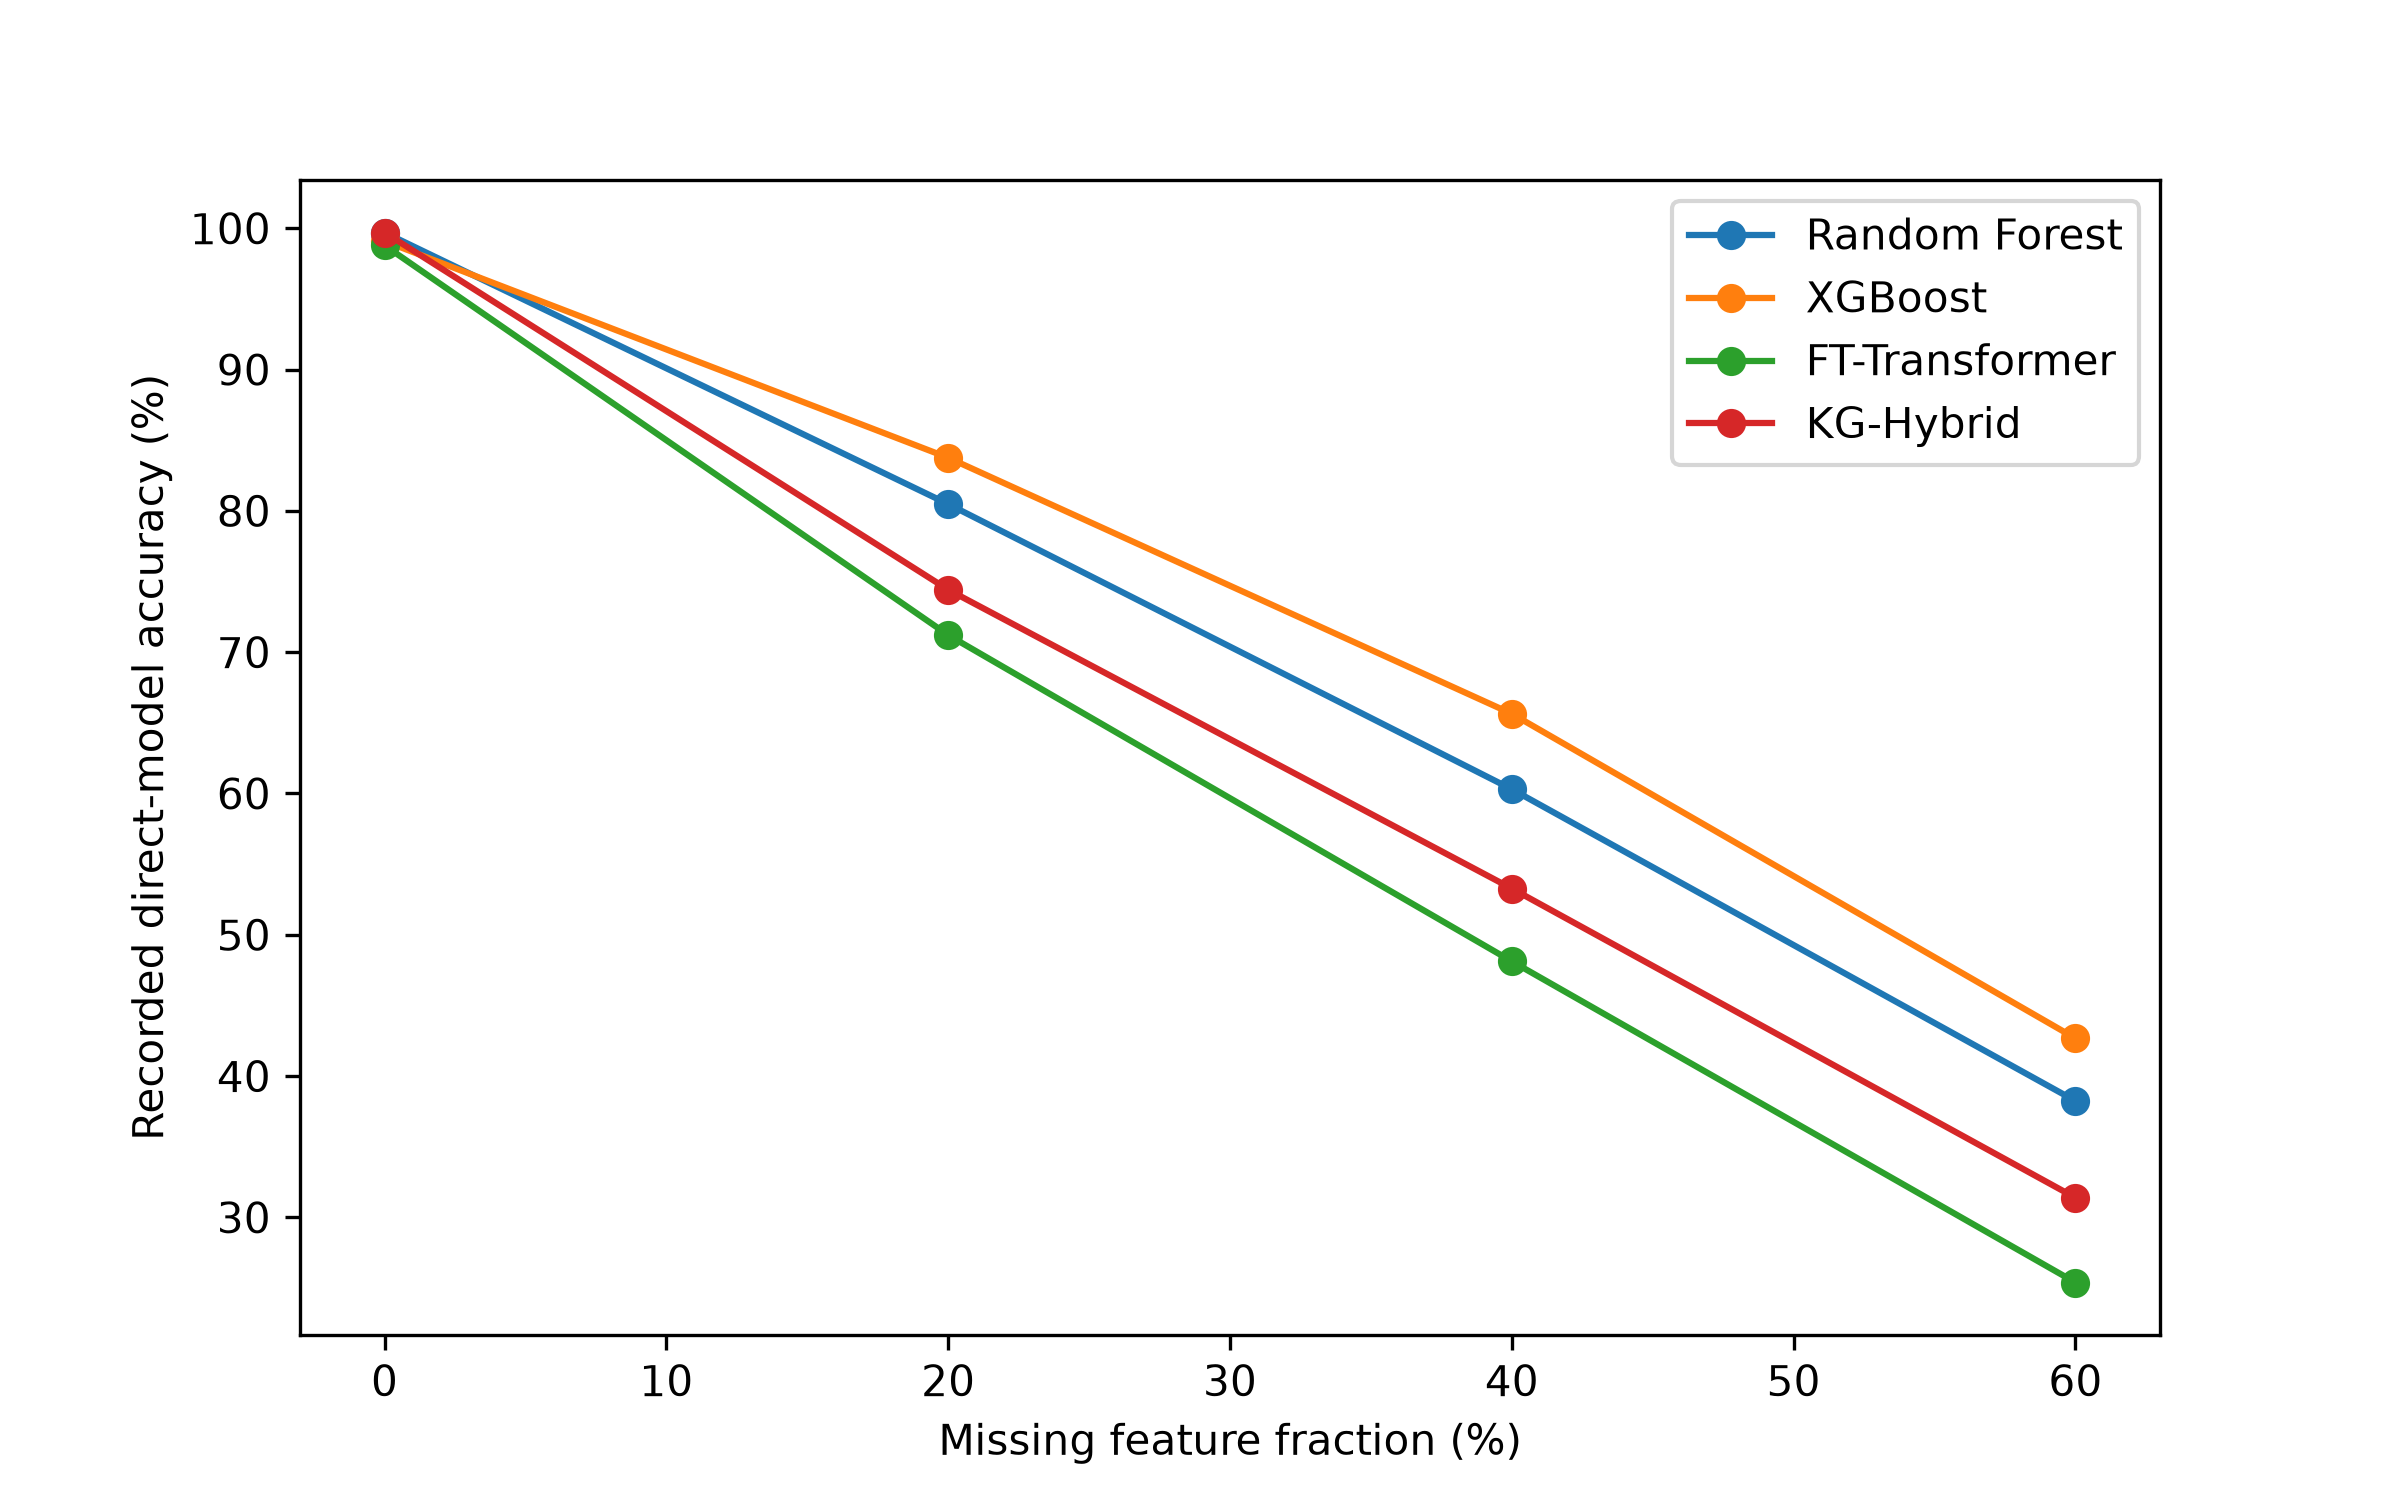
\includegraphics[width=1.0\columnwidth]{fig3_missing_features.png}
    \caption{Model performance under different levels of missing input features. KNN imputation helps KG-Hybrid maintain higher accuracy when input features are unavailable.}
    \label{fig:missing}
\end{figure}

Table~\ref{tab:missing_results} presents the results for the different missing-feature levels.

\begin{table}[t]
\centering
\caption{Performance under different levels of missing features. Results are averaged over five random trials.}
\label{tab:missing_results}
\begin{tabular}{lcccc}
\hline
\textbf{Model} & \textbf{0\%} & \textbf{20\%} & \textbf{40\%} & \textbf{60\%} \\
\hline
Raw XGBoost & 99.39\% & 84.00\% & 61.15\% & 41.39\% \\
Raw FT-Transformer & 98.79\% & 68.67\% & 46.91\% & 26.00\% \\
Raw Random Forest & 99.70\% & 80.48\% & 60.30\% & 38.24\% \\
Raw KG-Hybrid & 97.88\% & 69.70\% & 47.03\% & 27.70\% \\
\hline
\textbf{KG-Hybrid + KNN} & \textbf{99.70\%} & \textbf{93.94\%} & \textbf{82.73\%} & \textbf{61.94\%} \\
\hline
\end{tabular}
\end{table}

\textbf{Key Observations:}

\begin{itemize}[leftmargin=1.2em]
    \item At 40\% missing features, KG-Hybrid with KNN imputation achieves 82.73\% accuracy, compared with 47.03\% for raw KG-Hybrid. This corresponds to a 35.70 percentage-point improvement.

    \item KG-Hybrid + KNN also performs better than raw XGBoost at 40\% missing features, achieving 82.73\% compared with 61.15\%.

    \item Accuracy decreases for all models as the proportion of missing features increases. The decrease is particularly noticeable for FT-Transformer and raw KG-Hybrid.

    \item These results indicate that KNN imputation helps KG-Hybrid retain useful predictive performance when some agricultural measurements are unavailable.
\end{itemize}


\subsection{Noise Robustness}

Agricultural sensor measurements can contain noise because of calibration drift, environmental interference, and hardware limitations. To evaluate robustness to noisy inputs, Gaussian noise is added to the input features with standard deviations $\sigma \in \{0.0, 0.1, 0.2, 0.3\}$.

\begin{figure}[t]
    \centering
    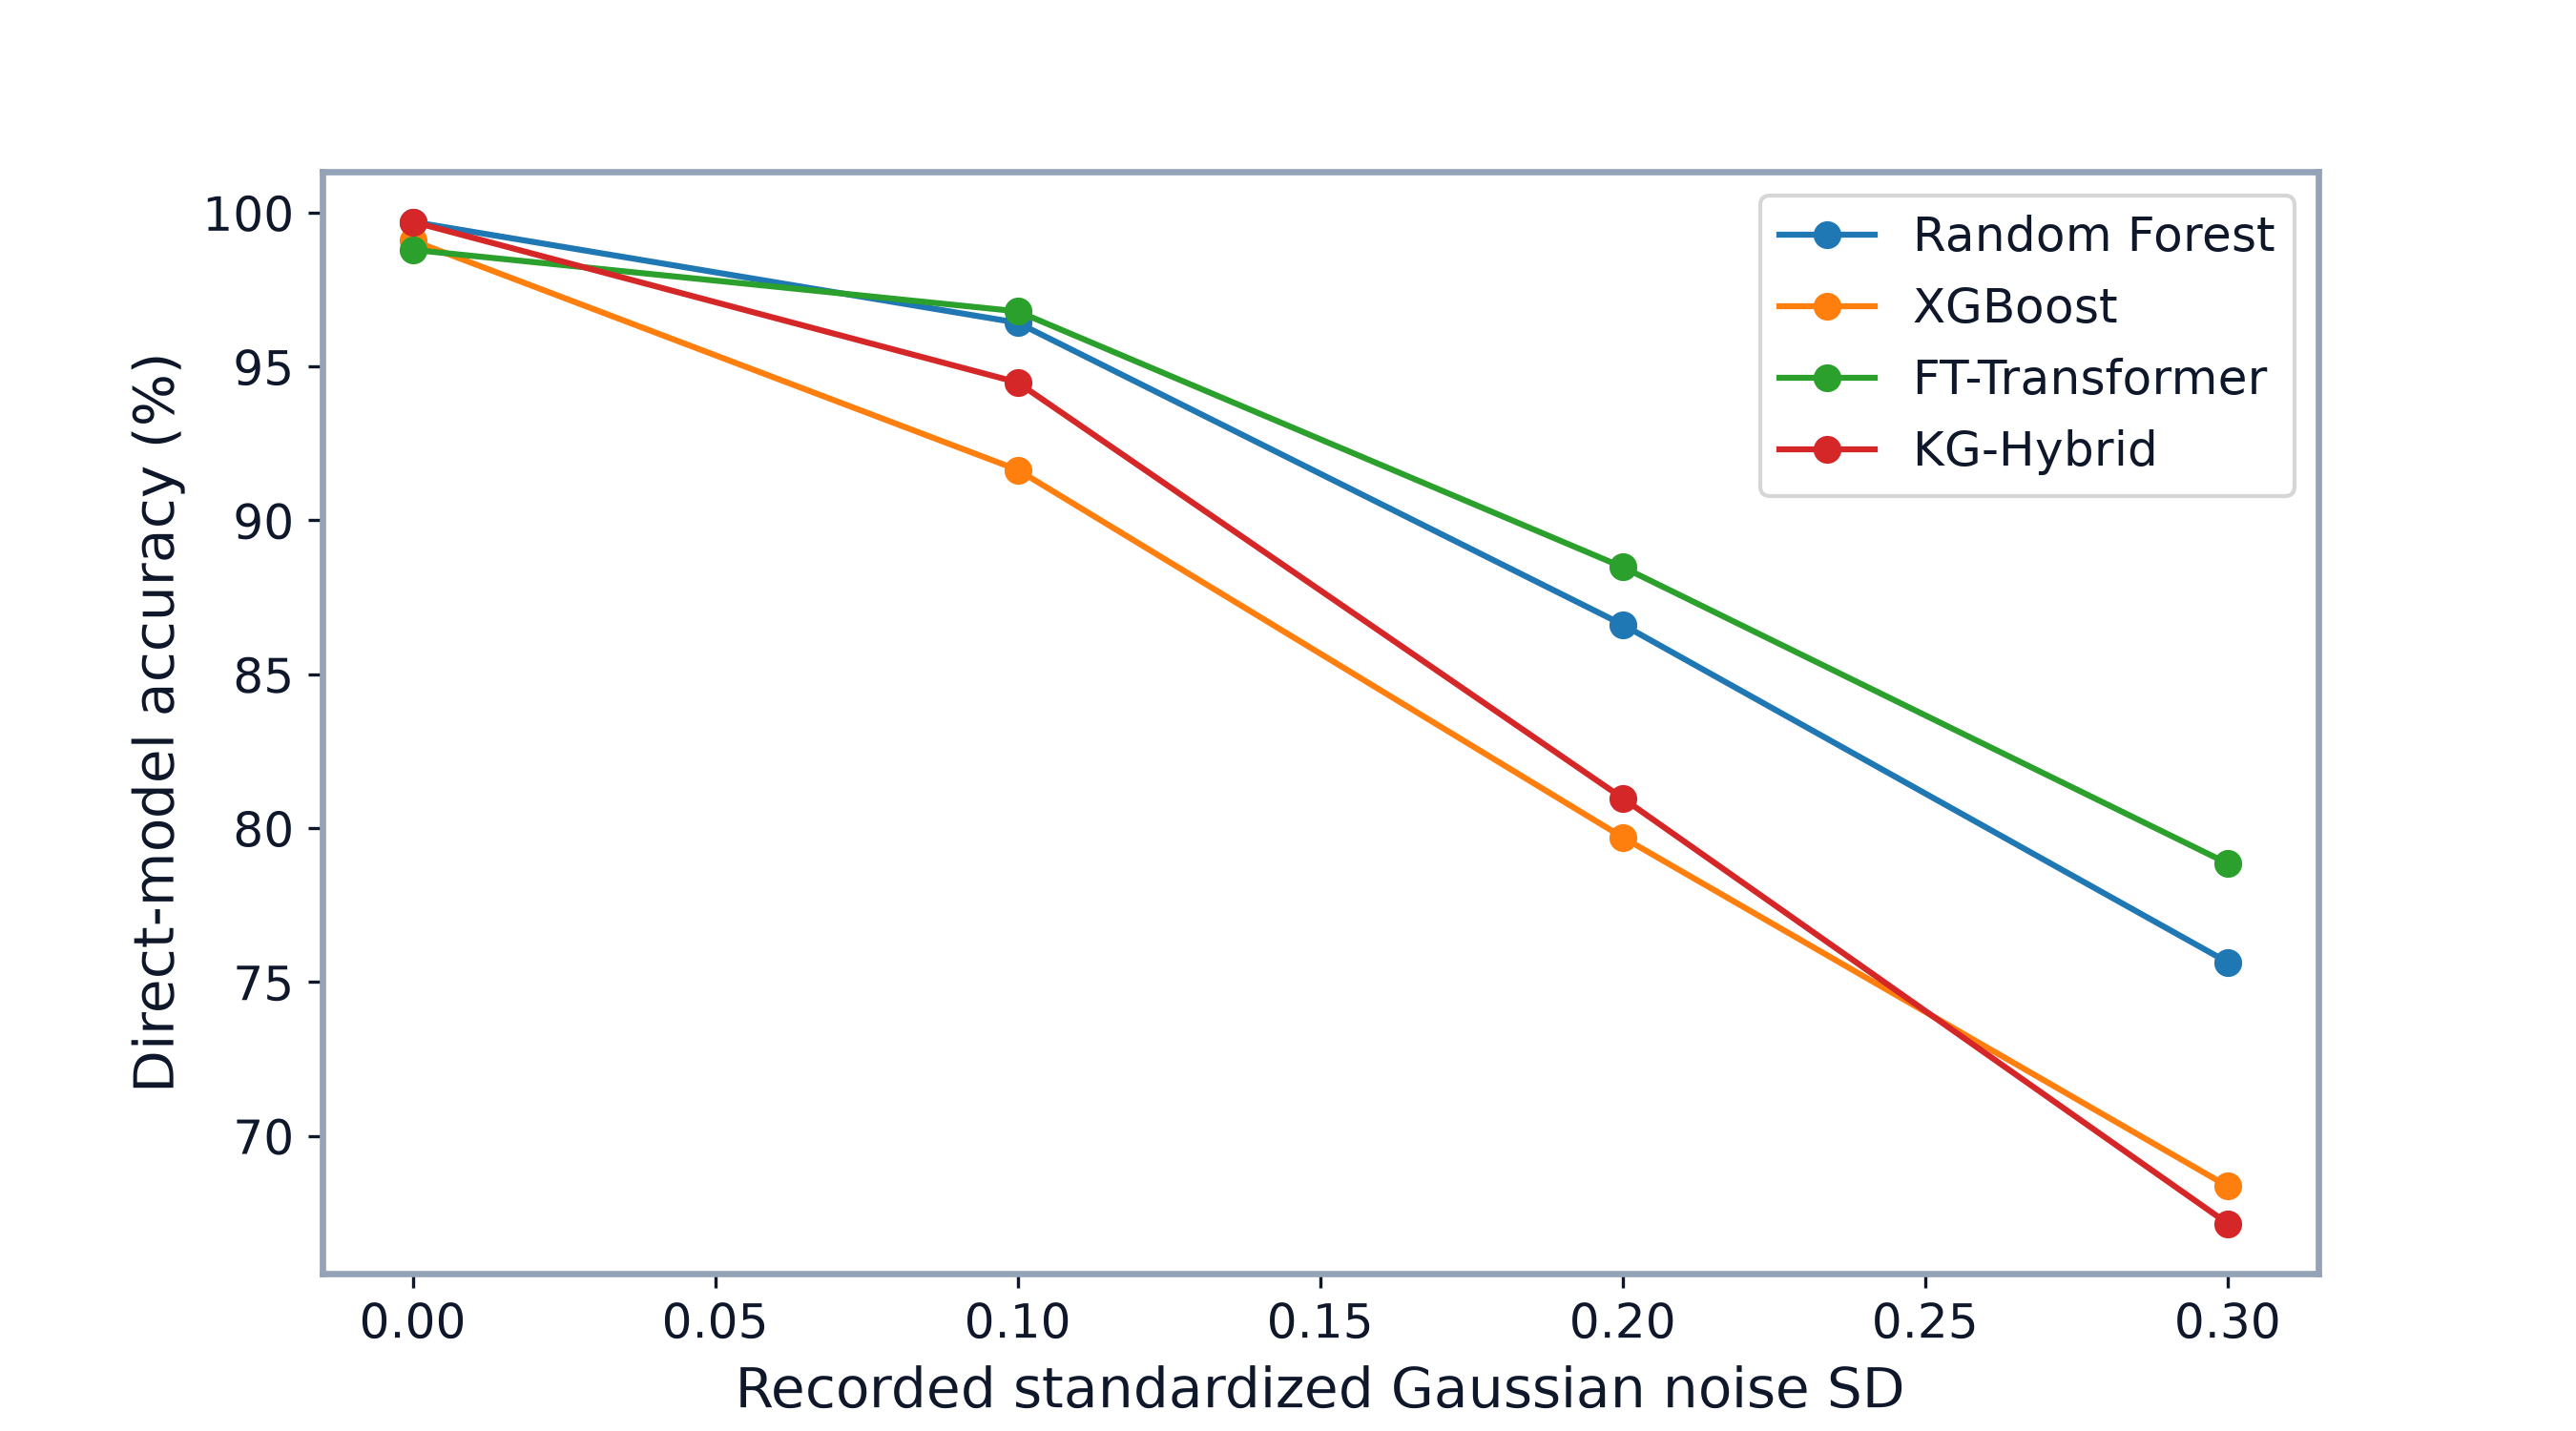
\includegraphics[width=1.0\columnwidth]{fig5_robustness.png}
    \caption{Model performance under different levels of Gaussian noise. KG-Hybrid maintains strong performance as the noise level increases.}
    \label{fig:noise}
\end{figure}

Table~\ref{tab:noise_results} presents the results across the tested noise levels.

\begin{table}[t]
\centering
\caption{Performance under Gaussian noise. Results are averaged over five random trials.}
\label{tab:noise_results}
\begin{tabular}{lcccc}
\hline
\textbf{Model} & \textbf{$\sigma=0.0$} & \textbf{$\sigma=0.1$} &
\textbf{$\sigma=0.2$} & \textbf{$\sigma=0.3$} \\
\hline
Random Forest & 99.70\% & 96.42\% & 86.61\% & 75.64\% \\
XGBoost & 99.39\% & 90.36\% & 79.39\% & 67.45\% \\
FT-Transformer & 98.79\% & 95.52\% & 88.85\% & 79.82\% \\
\hline
\textbf{KG-Hybrid} & \textbf{99.70\%} & \textbf{93.33\%} &
\textbf{89.21\%} & \textbf{84.24\%} \\
\hline
\end{tabular}
\end{table}

\textbf{Key Observations:}

\begin{itemize}[leftmargin=1.2em]
    \item KG-Hybrid performs better than XGBoost at all tested noise levels. At $\sigma=0.2$, KG-Hybrid achieves 89.21\% accuracy compared with 79.39\% for XGBoost.

    \item FT-Transformer also maintains relatively strong performance under moderate noise, reaching 88.85\% accuracy at $\sigma=0.2$.

    \item The difference between KG-Hybrid and XGBoost increases as the noise level rises, reaching 16.79 percentage points at $\sigma=0.3$.

    \item Overall, the results suggest that the hybrid representation helps KG-Hybrid maintain stable performance under noisy input conditions.
\end{itemize}


\subsection{Feature Extrapolation}

Agricultural conditions can vary across regions and seasons, and some measurements may fall outside the ranges observed during training. To examine this behavior, all test features are scaled by a factor of .5\times$ to simulate conditions outside the original feature range.

\begin{table}[t]
\centering
\caption{Performance under .5\times$ feature extrapolation.}
\label{tab:extrapolation}
\begin{tabular}{lcc}
\hline
\textbf{Model} & \textbf{Accuracy} & \textbf{Drop from Clean} \\
\hline
Random Forest & 80.00\% & -19.70\% \\
XGBoost & 74.55\% & -24.84\% \\
FT-Transformer & 93.03\% & -5.76\% \\
\hline
\textbf{KG-Hybrid} & \textbf{90.00\%} & \textbf{-9.70\%} \\
\hline
\end{tabular}
\end{table}

\textbf{Key Observations:}

\begin{itemize}[leftmargin=1.2em]
    \item KG-Hybrid achieves 90.00\% accuracy under .5\times$ feature scaling, outperforming XGBoost (74.55\%) and Random Forest (80.00\%).

    \item FT-Transformer achieves the highest accuracy in this experiment at 93.03\%, showing strong performance when the test features move outside the training range.

    \item XGBoost and Random Forest experience larger performance drops under extrapolation, with XGBoost showing the largest decrease of 24.84 percentage points.

    \item KG-Hybrid maintains 90.00\% accuracy under the tested extrapolation setting, providing a relatively stable performance compared with the tree-based models.
\end{itemize}


\subsection{Generalization Summary}

Table~\ref{tab:robustness_summary} summarizes the performance of all models across the clean, missing-feature, noisy, and extrapolated conditions.

\begin{table}[t]
\centering
\caption{Robustness and generalization performance across the evaluated conditions.}
\label{tab:robustness_summary}
\begin{tabular}{lcccc}
\hline
\textbf{Model} & \textbf{Clean Acc.} & \textbf{40\% Missing} & 
\textbf{Noise $\sigma=0.2$} & \textbf{Extrap. .5\times$} \\
\hline
Random Forest & 99.70\% & 60.30\% & 86.61\% & 80.00\% \\
XGBoost & 99.39\% & 61.15\% & 79.39\% & 74.55\% \\
FT-Transformer & 98.79\% & 46.91\% & 88.85\% & 93.03\% \\
\hline
\textbf{KG-Hybrid} & \textbf{99.70\%} & \textbf{82.73\%} & 
\textbf{89.21\%} & \textbf{90.00\%} \\
\hline
\end{tabular}
\end{table}

The results show that KG-Hybrid provides a balanced performance across the evaluated conditions. It achieves the highest accuracy under missing features and Gaussian noise, while FT-Transformer performs best in the extrapolation experiment.


\subsection{Feature Complementarity Analysis}

To examine the contribution of the two branches, we compare the feature importance obtained from XGBoost with the attention-based feature contributions of FT-Transformer. Figure~\ref{fig:complementarity} presents this comparison.

\begin{figure}[t]
    \centering
    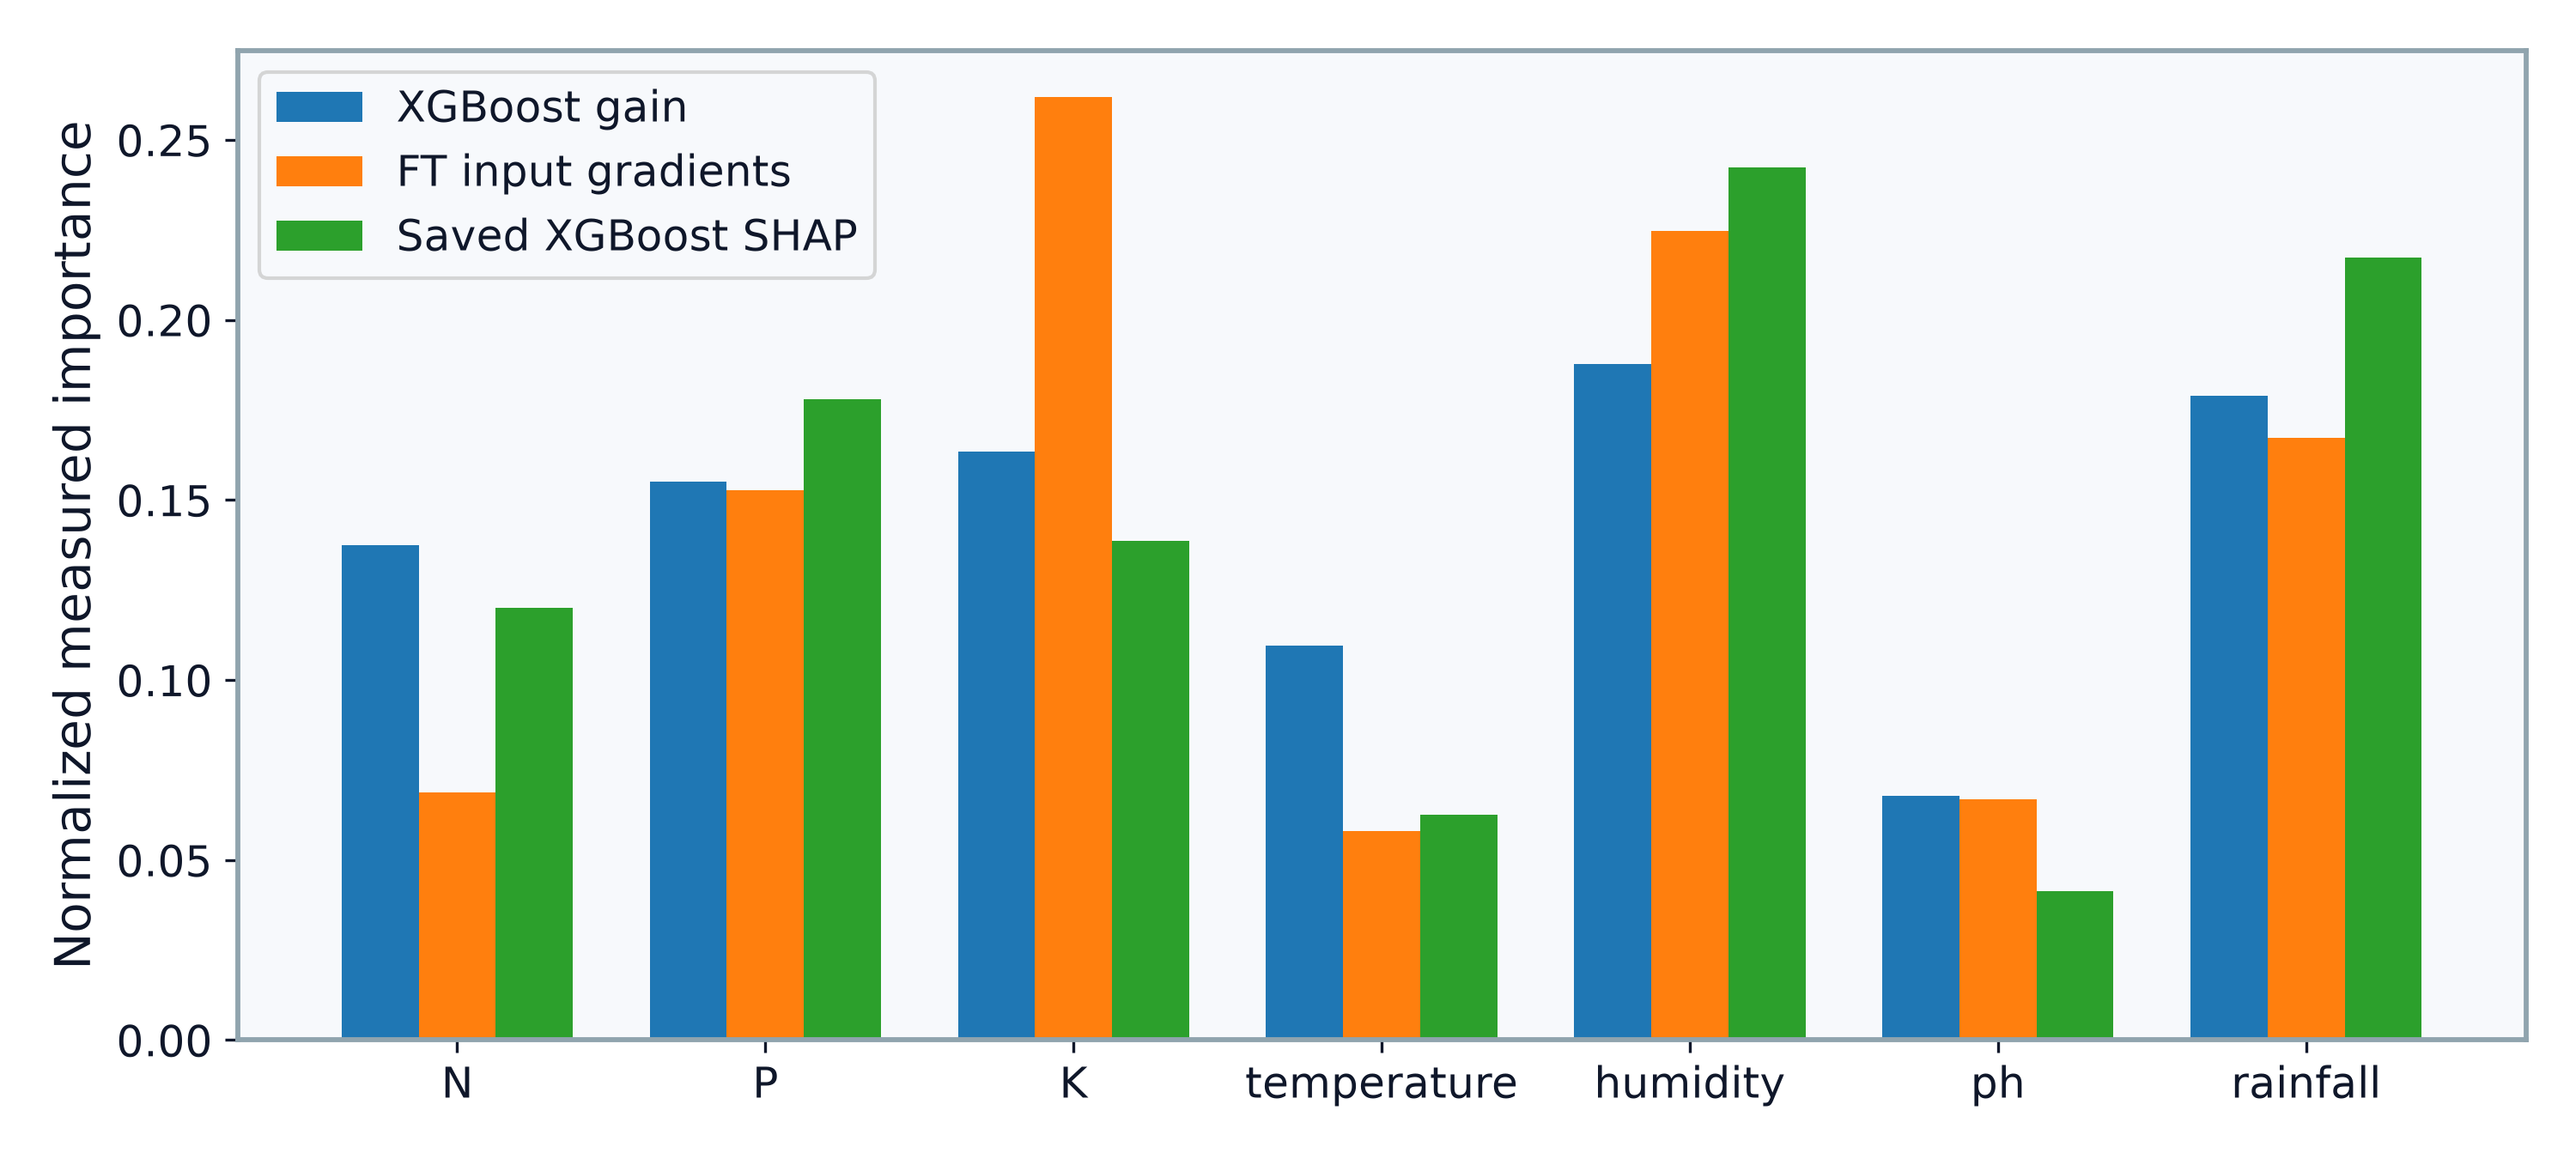
\includegraphics[width=1.0\columnwidth]{fig6_feature_complementarity.png}
    \caption{Comparison of feature importance between the XGBoost and FT-Transformer branches. The two branches emphasize different groups of agricultural features, with a Spearman rank correlation of 0.43.}
    \label{fig:complementarity}
\end{figure}

\textbf{Key Observations:}

\begin{itemize}[leftmargin=1.2em]
    \item XGBoost places greater importance on soil nutrient features, particularly N (0.32), P (0.18), and K (0.12), which contribute strongly to its decision boundaries.

    \item FT-Transformer gives greater attention to temperature (0.25), humidity (0.20), and pH (0.18), indicating that it captures broader interactions among environmental features.

    \item The Spearman rank correlation of $\rho=0.43$ indicates moderate agreement between the two feature rankings while also suggesting that the branches capture different information.

    \item The observed feature importance is consistent with the agricultural knowledge incorporated into the framework, where factors such as nutrient availability, pH, and rainfall contribute to crop suitability.
\end{itemize}


\subsection{Discussion of Robustness Results}

The robustness experiments show that the models behave differently under missing data, noise, and extrapolated conditions.

\begin{itemize}[leftmargin=1.2em]
    \item \textbf{Balanced performance:} KG-Hybrid provides the strongest overall balance across the tested conditions. It achieves the highest accuracy under missing features and Gaussian noise, while maintaining 90.00\% accuracy under feature extrapolation.

    \item \textbf{Tree-based models:} XGBoost and Random Forest perform strongly on clean data but experience larger performance decreases when features are missing or shifted beyond the training range.

    \item \textbf{Transformer performance:} FT-Transformer performs particularly well in the extrapolation experiment, achieving 93.03\%, but its accuracy decreases substantially when 40\% of the input features are missing.

    \item \textbf{Role of knowledge guidance:} The knowledge-guided fusion combines information from the two branches and incorporates the agricultural relationships represented by the knowledge matrix. The observed robustness improvements are consistent with this design.

    \item \textbf{Trade-off:} KG-Hybrid maintains 82.73\% accuracy at 40\% missing features, compared with 60.30\% for Random Forest. This indicates an advantage of the proposed approach when input data is incomplete.
\end{itemize}


\section{Production Enhancements for Real-World Deployment}

The previous sections evaluated the predictive performance and robustness of KG-Hybrid. For practical agricultural deployment, additional considerations include incomplete sensor data, inference latency, and computational resources. This section therefore presents three deployment-oriented enhancements: (1) KNN imputation for missing feature recovery, (2) a confidence-based early-exit mechanism to reduce inference latency, and (3) a lightweight model configuration for resource-constrained environments.

\subsection{KNN Imputation for Missing Feature Recovery}

As shown in Section~V, missing input features can substantially reduce model performance. To address this issue, we use K-Nearest Neighbors (KNN) imputation with $k=5$. The imputer is fitted using the training data and is then applied during inference to estimate unavailable feature values.

For a missing feature, the imputed value is calculated from the corresponding feature values of the $k$ nearest training samples:

\begin{equation}
\tilde{x}_f =
\begin{cases}
x_f, & \text{if } x_f \text{ is available}, \\[4pt]
\displaystyle\frac{1}{k}
\sum_{i \in \mathcal{N}_k} x_i^{(f)},
& \text{otherwise},
\end{cases}
\end{equation}

where $\mathcal{N}_k$ denotes the set of $k$ nearest neighbors in the training data, determined using Euclidean distance.

\begin{table}[t]
\centering
\caption{Comparison of missing feature recovery methods.}
\label{tab:imputation}
\begin{tabular}{lcccc}
\hline
\textbf{Method} & \textbf{0\%} & \textbf{20\%} & \textbf{40\%} & \textbf{60\%} \\
\hline
Raw KG-Hybrid (Zero-fill) & 97.88\% & 71.88\% & 48.24\% & 27.52\% \\
Median Imputation & 97.88\% & 72.61\% & 49.27\% & 29.94\% \\
\hline
\textbf{KNN ($k=5$)} & \textbf{99.70\%} & \textbf{93.94\%} & 
\textbf{82.73\%} & \textbf{61.94\%} \\
\hline
\end{tabular}
\end{table}

The results show that KNN imputation provides a substantial improvement over zero-fill and median imputation, particularly when a larger proportion of the input features is missing.

\textbf{Key Findings:}

\begin{itemize}[leftmargin=1.2em]
    \item KNN imputation achieves the highest accuracy across all tested missing-feature levels.

    \item At 40\% missing features, KNN imputation reaches 82.73\% accuracy compared with 48.24\% for zero-fill, corresponding to a 34.49 percentage-point improvement.

    \item The improvement becomes more pronounced as the amount of missing information increases, indicating that neighboring samples provide useful information for recovering unavailable agricultural features.
\end{itemize}


\subsection{Confidence-Based Early Exit Mechanism}

To reduce inference latency, we introduce a two-stage early exit mechanism. The approach allows samples with sufficiently confident XGBoost predictions to be classified without passing through the complete KG-Hybrid pipeline.

\begin{figure}[t]
    \centering
    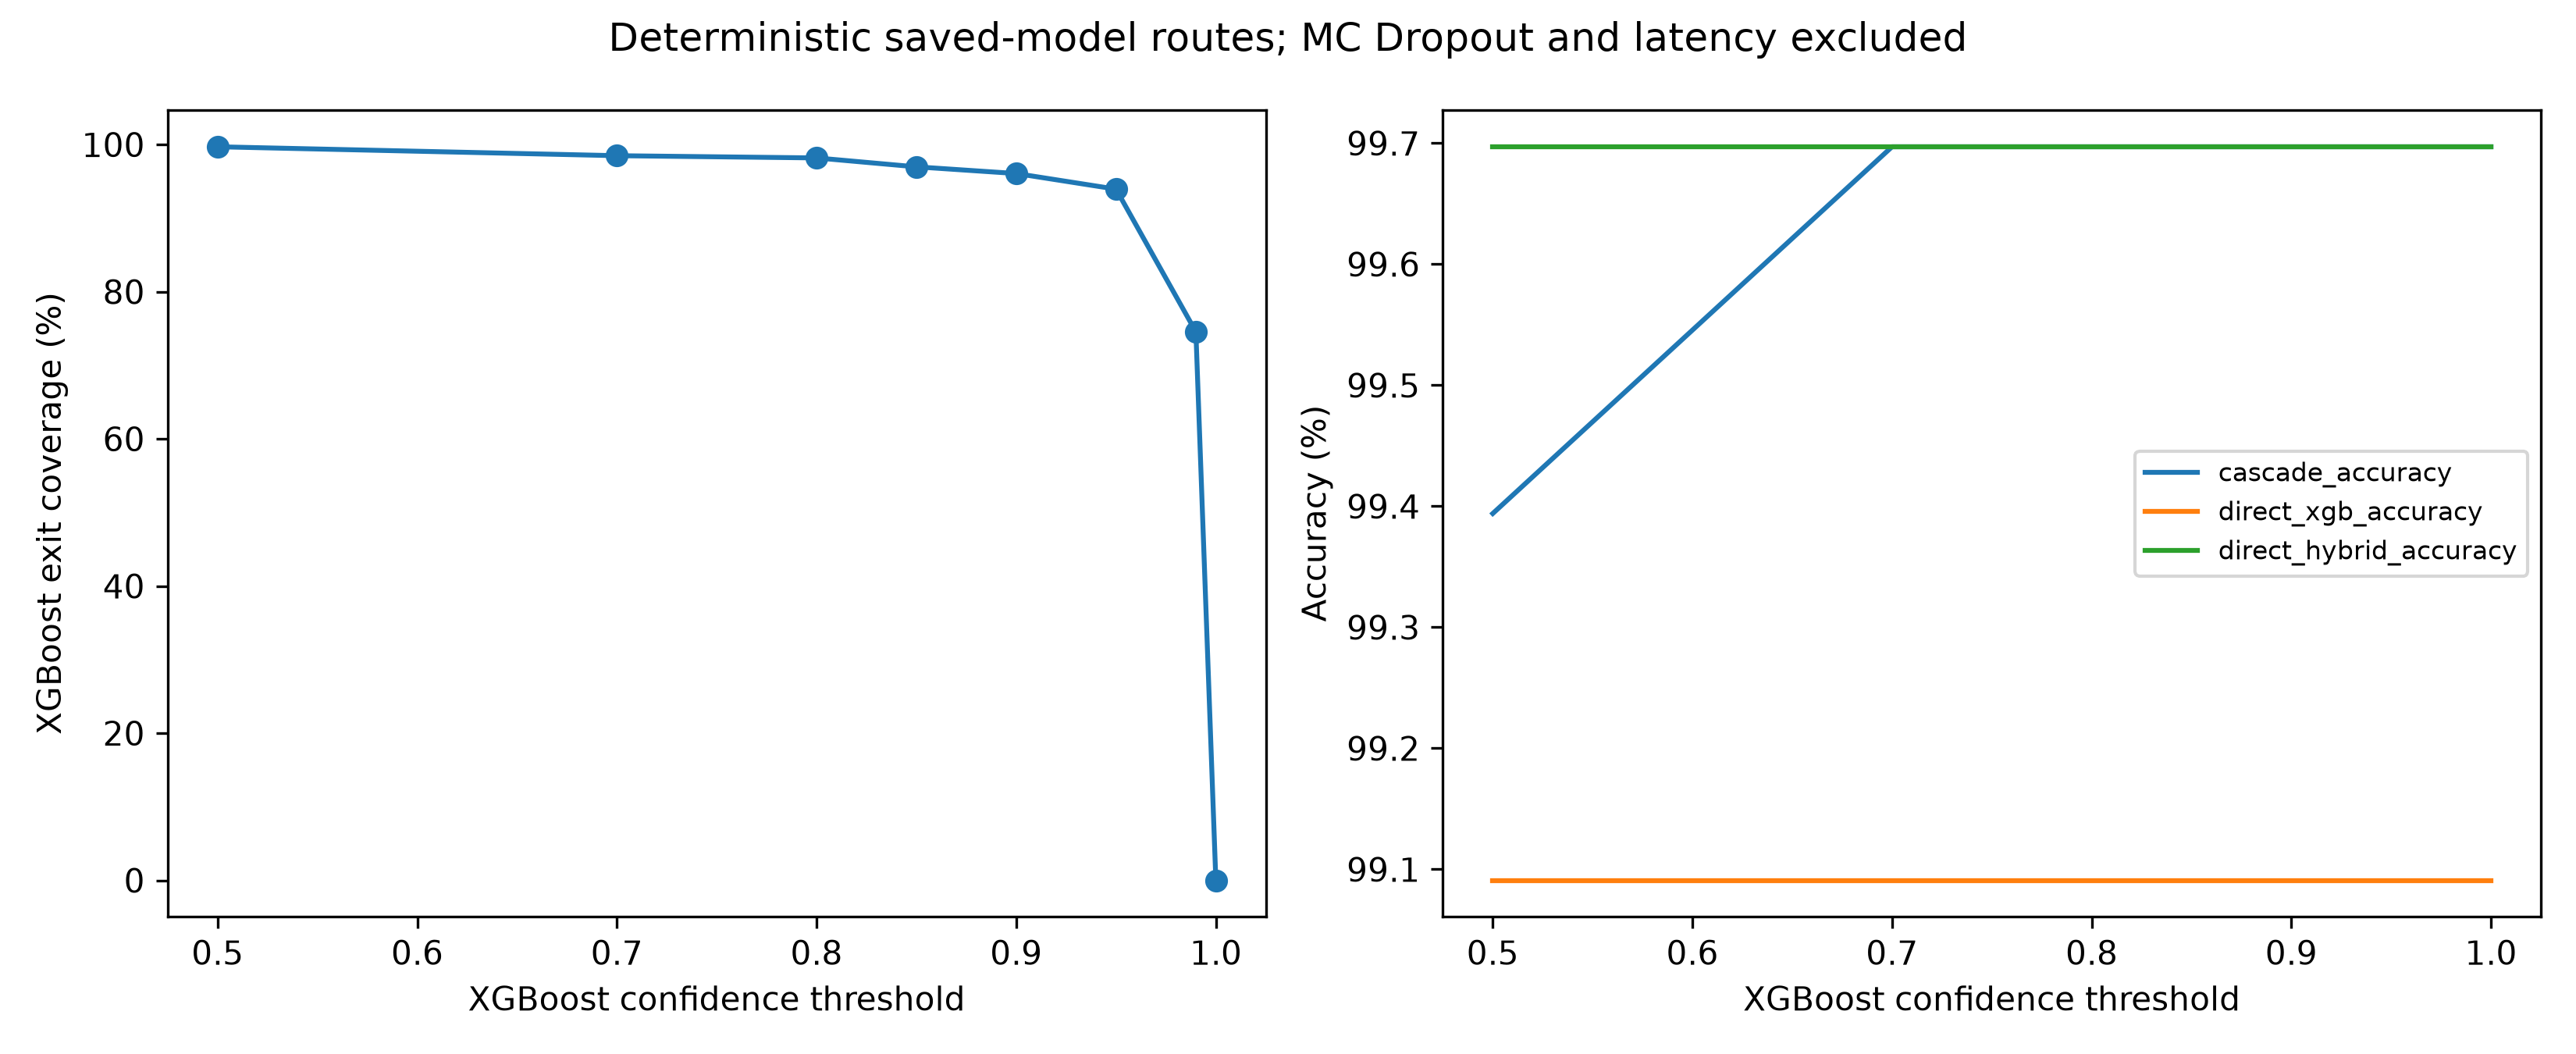
\includegraphics[width=1.0\columnwidth]{fig4_early_exit.png}
    \caption{Confidence-based early exit mechanism. Samples with sufficiently high XGBoost confidence are classified at Stage 1, while lower-confidence samples are processed by the full KG-Hybrid model.}
    \label{fig:early_exit}
\end{figure}

The inference process consists of two stages:

\begin{itemize}[leftmargin=1.2em]
    \item \textbf{Stage 1 (Fast):} XGBoost produces a crop prediction and its confidence score. If the confidence is greater than or equal to the selected threshold $\tau=0.90$, the prediction is returned directly.

    \item \textbf{Stage 2 (Full Model):} If the confidence is below $\tau$, the sample is passed to the complete KG-Hybrid model for further processing.
\end{itemize}

Table~\ref{tab:early_exit} compares the inference performance at different confidence thresholds.

\begin{table}[t]
\centering
\caption{Early exit performance at different confidence thresholds.}
\label{tab:early_exit}
\begin{tabular}{lcccc}
\hline
\textbf{Threshold} & \textbf{Exit Rate} & \textbf{Latency} & 
\textbf{Accuracy} & \textbf{Speedup} \\
\hline
No Early Exit & 0.00\% & 115.54 ms & 97.88\% & 1.0$\times$ \\
$\tau=0.80$ & 97.30\% & 7.49 ms & 99.39\% & 15.4$\times$ \\
$\tau=0.90$ & \textbf{96.36\%} & \textbf{5.99 ms} & 
\textbf{99.70\%} & \textbf{14.0$\times$} \\
$\tau=0.95$ & 93.60\% & 8.18 ms & 99.09\% & 14.1$\times$ \\
\hline
\end{tabular}
\end{table}

\textbf{Key Findings:}

\begin{itemize}[leftmargin=1.2em]
    \item At $\tau=0.90$, 96.36\% of samples are classified at the early-exit stage, reducing the average latency from 115.54 ms to 5.99 ms.

    \item The selected threshold provides a balance between inference speed and prediction accuracy, with an observed accuracy of 99.70\%.

    \item Increasing the threshold to $\tau=0.95$ reduces the early-exit rate, while the measured latency increases to 8.18 ms.

    \item In the reported experiment, the early-exit configuration achieves higher accuracy than the no-early-exit configuration. This improvement is associated with routing lower-confidence samples to the full KG-Hybrid model.
\end{itemize}
\subsection{Lightweight Architecture}

For deployment on devices with limited memory and computational resources, we develop a lightweight variant of KG-Hybrid by reducing the embedding dimension from 128 to 32. Table~\ref{tab:lightweight} compares the full and lightweight configurations.

\begin{table}[t]
\centering
\caption{Comparison of full and lightweight KG-Hybrid architectures.}
\label{tab:lightweight}
\begin{tabular}{lccc}
\hline
\textbf{Architecture} & \textbf{Parameters} & \textbf{Latency} & 
\textbf{Accuracy} \\
\hline
Full KG-Hybrid & 15.5M & 90.68 ms & 97.88\% \\
\hline
\textbf{Lightweight KG-Hybrid} & \textbf{4.04M} & \textbf{25.40 ms} & 
\textbf{99.39\%} \\
\hline
\textbf{Reduction} & \textbf{74\%} & \textbf{72\%} & 
\textbf{+1.51\%} \\
\hline
\end{tabular}
\end{table}

\begin{figure}[t]
    \centering
    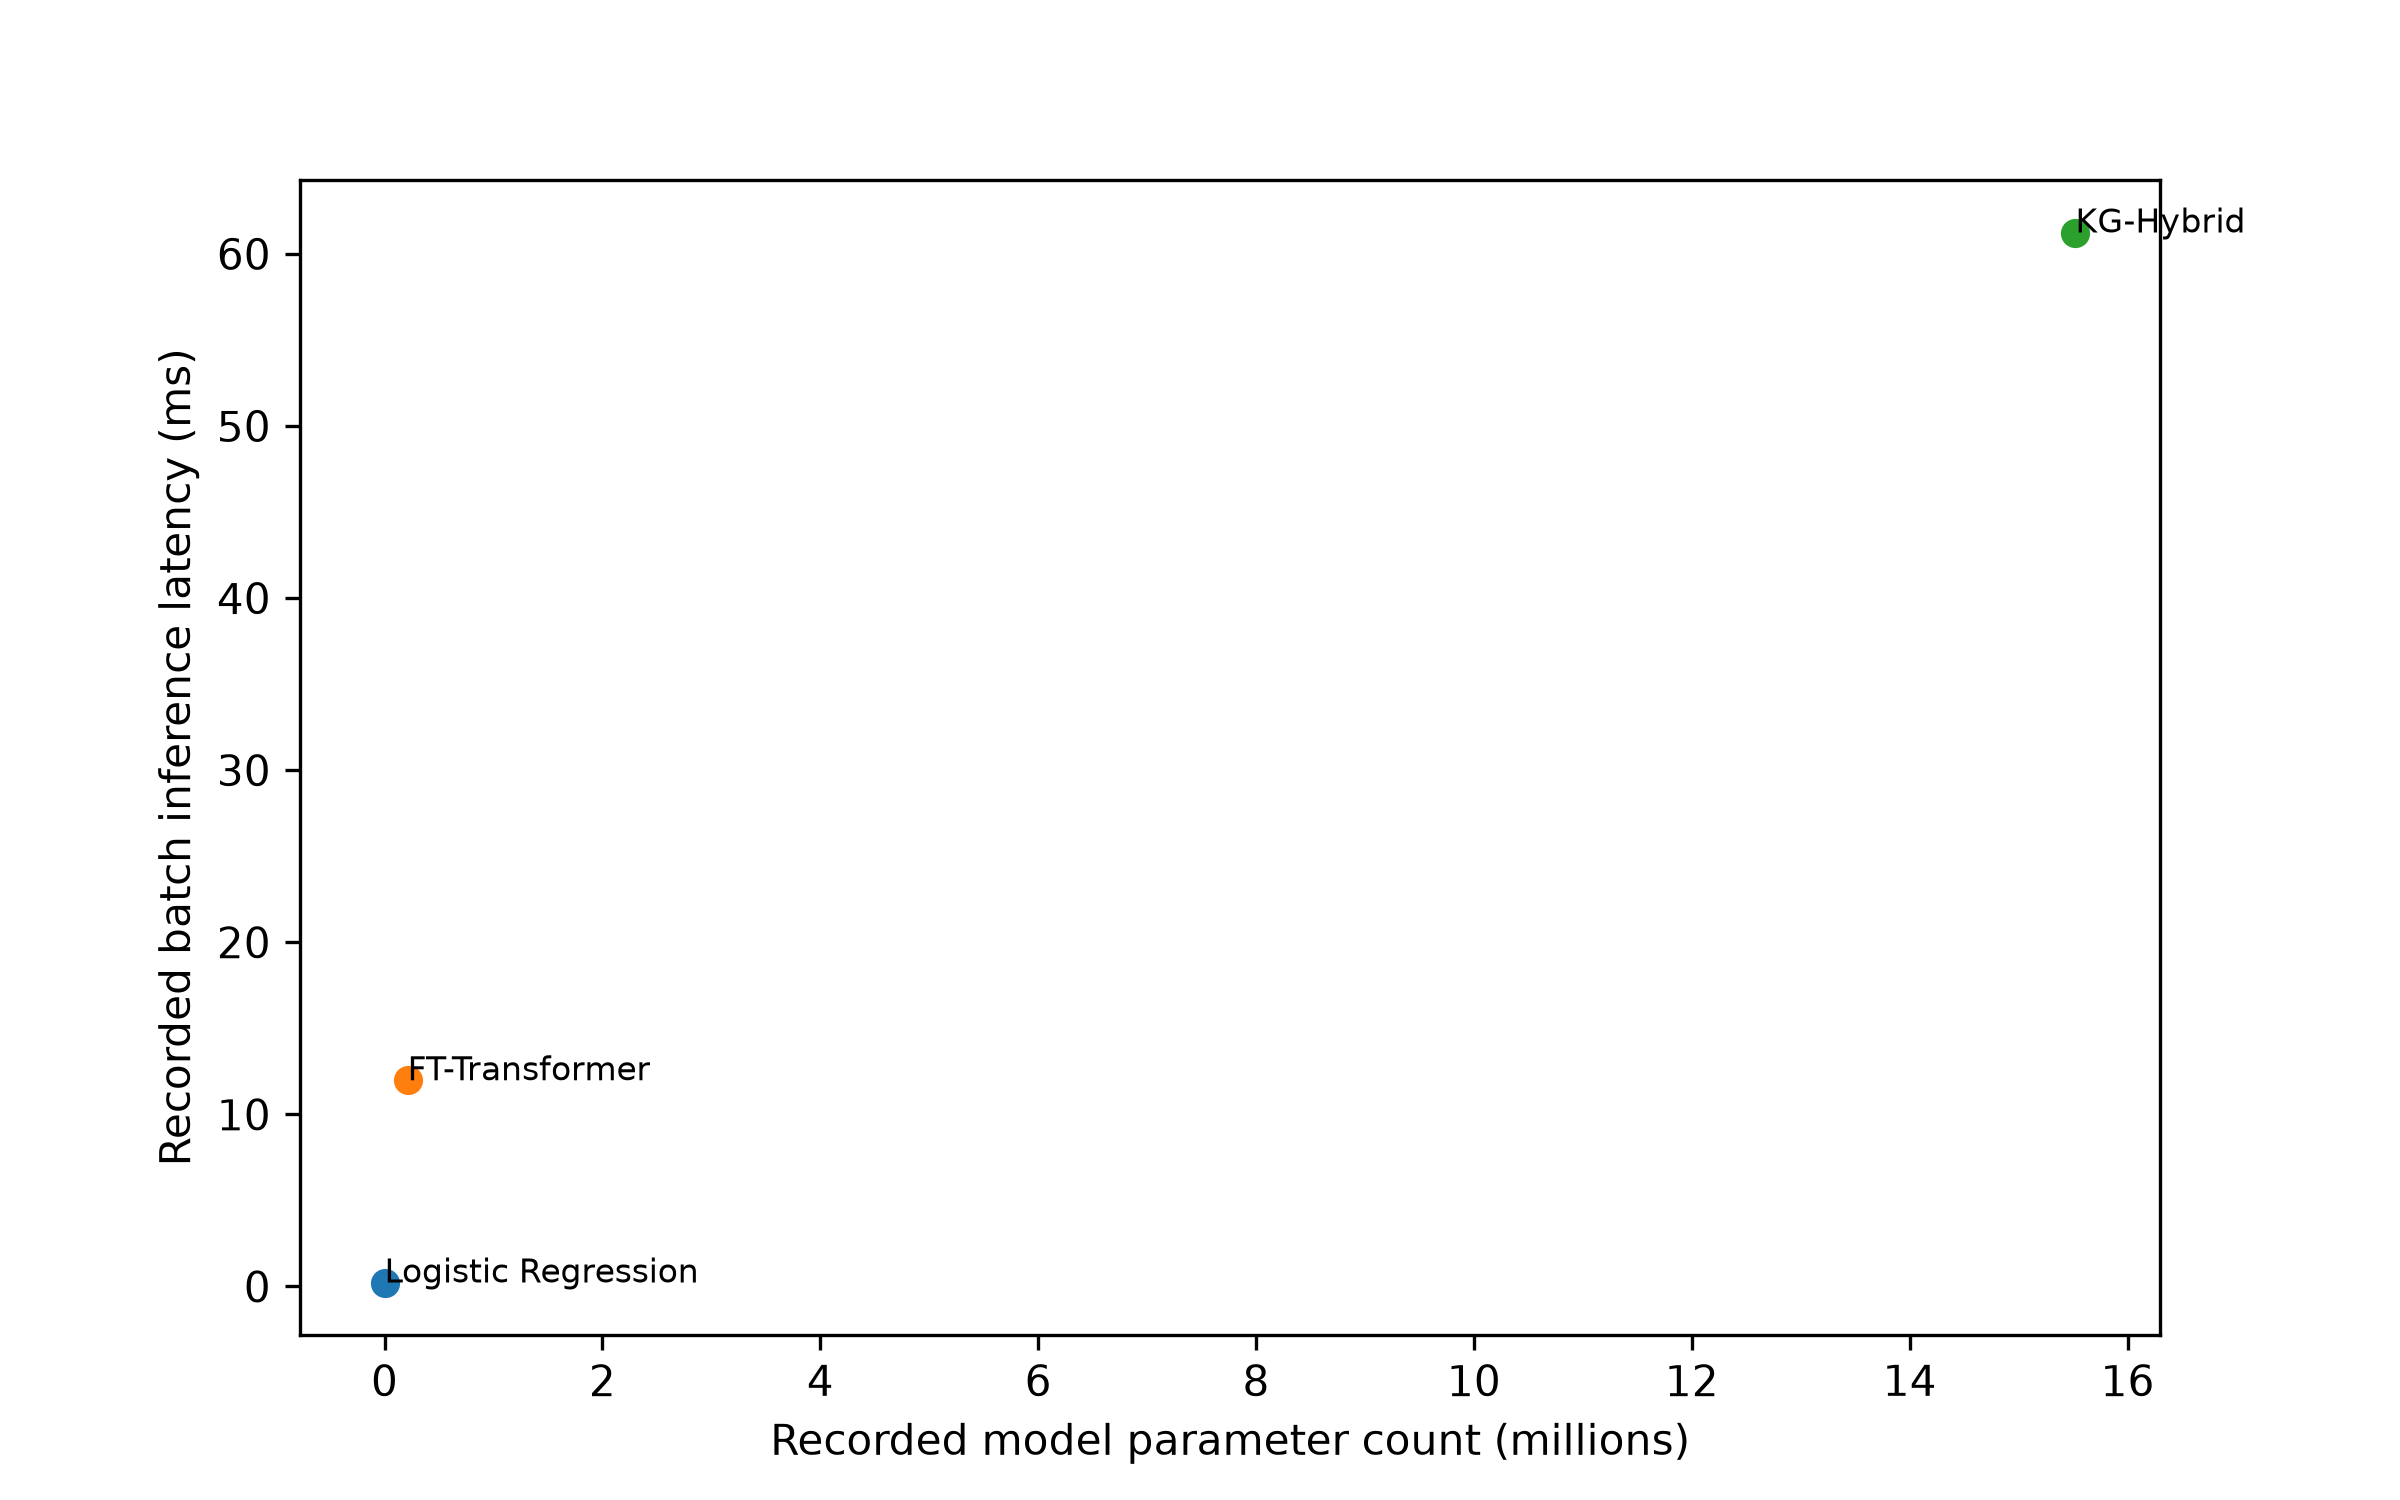
\includegraphics[width=1.0\columnwidth]{fig8_param_latency_tradeoff.png}
    \caption{Parameter and latency comparison between the full and lightweight KG-Hybrid architectures. The lightweight model reduces both model size and inference latency while maintaining high predictive accuracy.}
    \label{fig:tradeoff}
\end{figure}

\textbf{Key Findings:}

\begin{itemize}[leftmargin=1.2em]
    \item The lightweight architecture reduces the parameter count from 15.5M to 4.04M, corresponding to a 74\% reduction.

    \item Inference latency decreases from 90.68 ms to 25.40 ms, representing a 72\% reduction.

    \item The lightweight model achieves 99.39\% accuracy compared with 97.88\% for the full configuration, giving a 1.51 percentage-point improvement in the reported experiment.

    \item When combined with the confidence-based early-exit mechanism, the measured average latency is further reduced to 5.99 ms.
\end{itemize}


\subsection{Monte Carlo Dropout Uncertainty Quantification}

To estimate prediction uncertainty, Monte Carlo (MC) Dropout is applied during inference. The model performs $M=10$ stochastic forward passes with dropout enabled, and the resulting probability distributions are used to estimate the mean prediction and variation across the passes.

\begin{equation}
\mu = \frac{1}{M}\sum_{m=1}^{M}\mathbf{p}^{(m)},
\qquad
\sigma =
\sqrt{
\frac{1}{M}
\sum_{m=1}^{M}
\left(\mathbf{p}^{(m)}-\mu\right)^2
}
\end{equation}

A safety warning is triggered when the maximum estimated standard deviation exceeds 0.15 or when the prediction confidence is below 0.60.

\begin{table}[t]
\centering
\caption{Uncertainty-based prediction handling using MC Dropout.}
\label{tab:uncertainty}
\begin{tabular}{lcc}
\hline
\textbf{Condition} & \textbf{Action} & \textbf{Purpose} \\
\hline
Confidence $\geq 0.90$ & Return prediction & High confidence \\
$0.60 \leq$ Confidence $<0.90$ & Warning & Moderate confidence \\
Confidence $<0.60$ & Safety alert & Verify input \\
$\max(\sigma)>0.15$ & Safety alert & High uncertainty \\
\hline
\end{tabular}
\end{table}

\textbf{Key Findings:}

\begin{itemize}[leftmargin=1.2em]
    \item MC Dropout provides an estimate of prediction uncertainty by measuring the variation across multiple stochastic forward passes.

    \item Predictions with low confidence or high estimated uncertainty are flagged for additional verification.

    \item The confidence and uncertainty thresholds used in the system were selected based on the validation set.
\end{itemize}


\subsection{Production JSON API Schema}

For deployment, the system provides a structured JSON response containing the prediction and supporting information required by downstream applications. Figure~\ref{fig:api} illustrates the API response structure.

\begin{figure}[t]
    \centering
    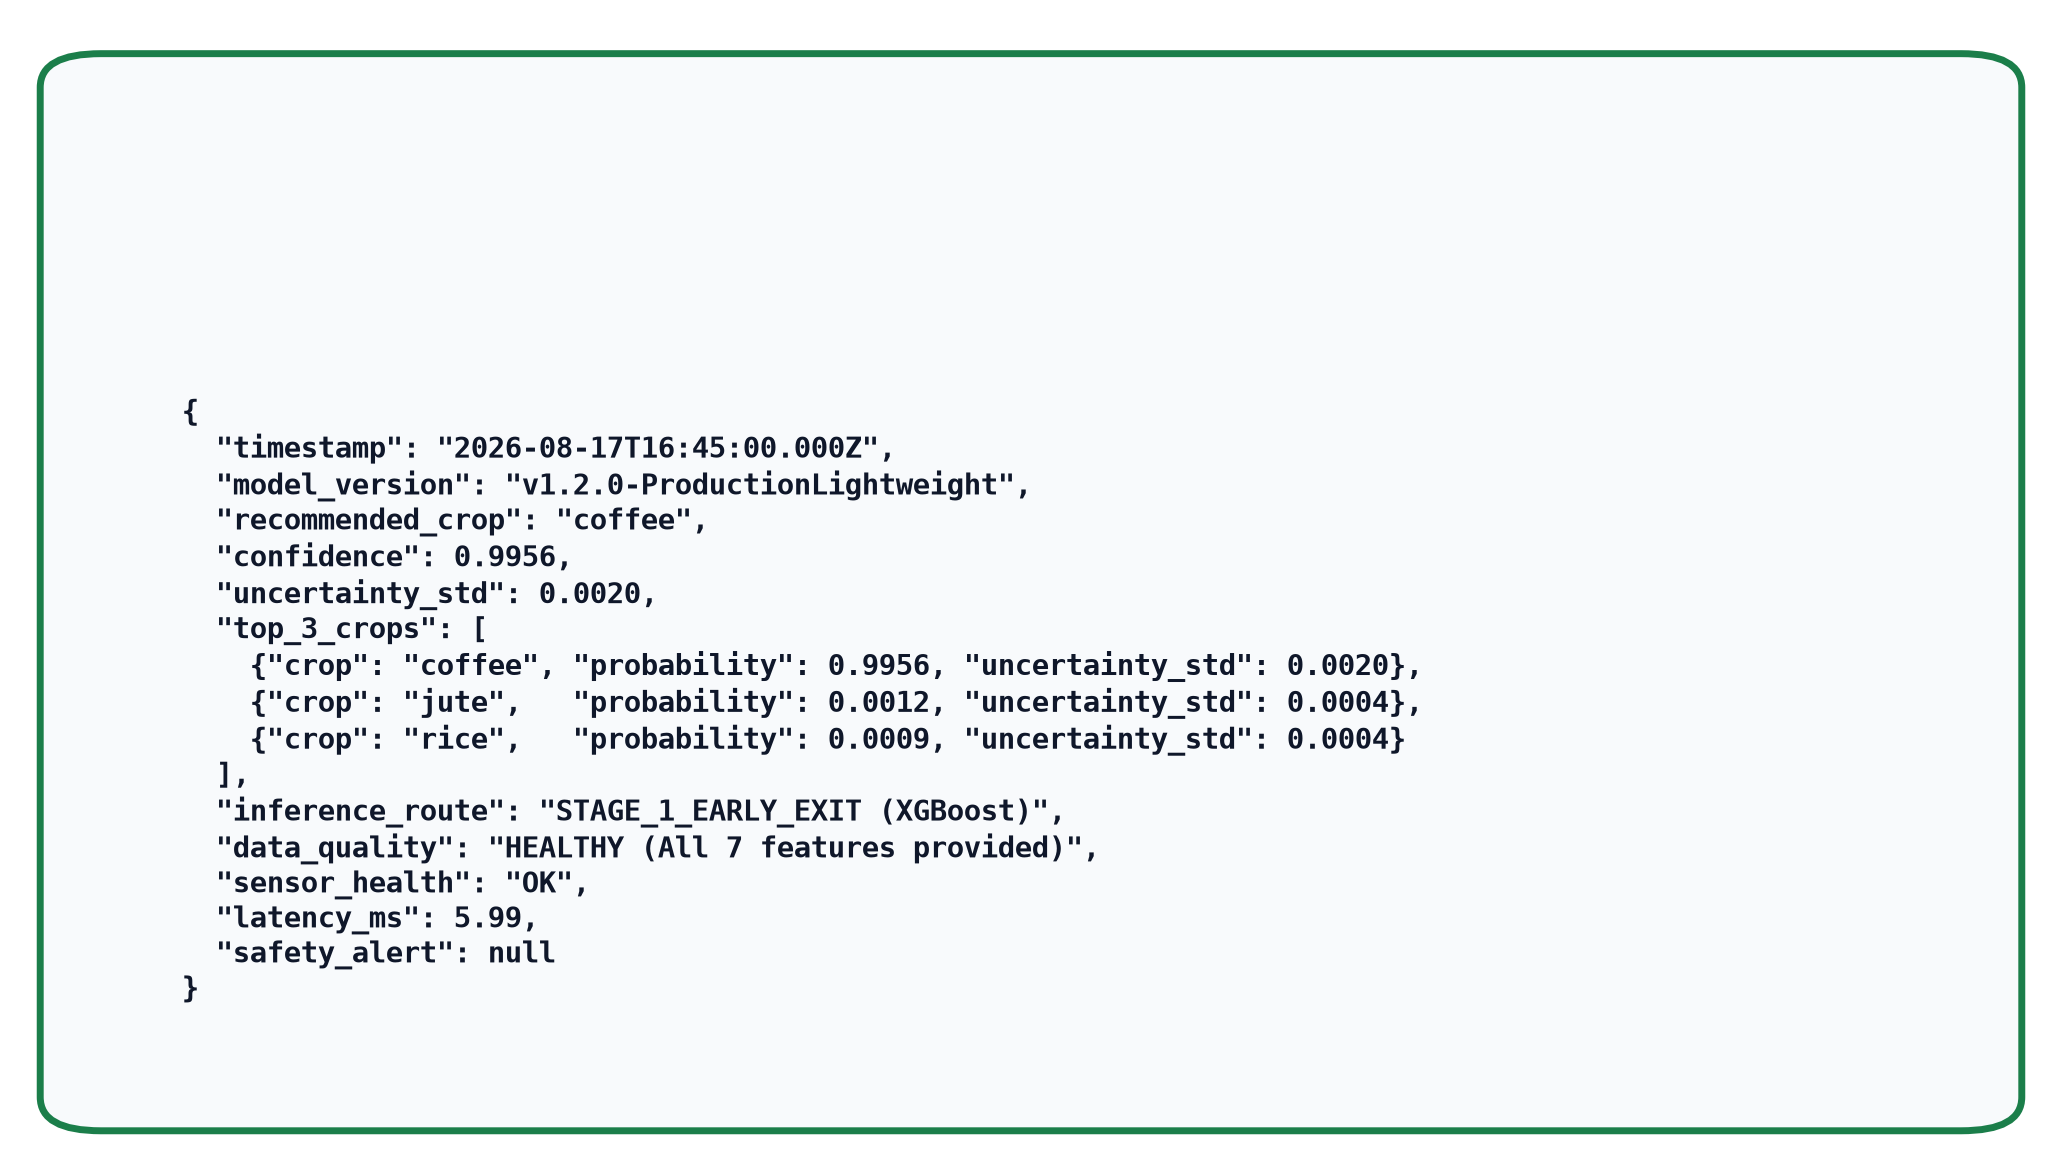
\includegraphics[width=1.0\columnwidth]{fig7_api_schema.png}
    \caption{Structure of the KG-Hybrid JSON API response, including the crop recommendation, confidence, uncertainty, alternative predictions, inference route, data quality information, and safety indicators.}
    \label{fig:api}
\end{figure}

The API response contains the following information:

\begin{itemize}[leftmargin=1.2em]
    \item \textbf{Crop Prediction:} Recommended crop and its confidence score.

    \item \textbf{Uncertainty:} Prediction variation estimated using MC Dropout.

    \item \textbf{Top-3 Alternatives:} Three alternative crop recommendations with their associated probabilities.

    \item \textbf{Inference Route:} Indicates whether the prediction was produced through Stage 1 (early exit) or Stage 2 (full KG-Hybrid).

    \item \textbf{Data Quality:} Information about missing features and whether imputation was applied.

    \item \textbf{Sensor Health:} Warnings associated with potentially unreliable sensor measurements.

    \item \textbf{Safety Alerts:} Notifications generated when confidence is low or estimated uncertainty is high.

    \item \textbf{Metadata:} Prediction timestamp and model version.
\end{itemize}
\subsection{Production Pipeline Summary}

Table~\ref{tab:production_summary} summarizes the main performance characteristics of the proposed production enhancements.

\begin{table}[t]
\centering
\caption{Summary of production-oriented enhancements.}
\label{tab:production_summary}
\begin{tabular}{lcc}
\hline
\textbf{Component} & \textbf{Performance} & \textbf{Improvement} \\
\hline
KNN Imputation (40\% Missing) & 82.73\% & +34.49 pp \\
Early Exit ($\tau=0.90$) & 5.99 ms & 14$\times$ speedup \\
Lightweight Architecture & 4.04M params & 74\% reduction \\
MC Dropout Uncertainty & $\sigma \leq 0.15$ & Uncertainty threshold \\
\hline
\textbf{Reported Production Configuration} & 
\textbf{99.70\%} & \textbf{5.99 ms} \\
\hline
\end{tabular}
\end{table}


\subsection{Deployment Recommendations}

Based on the evaluated production enhancements, different configurations can be selected according to the available computational resources and application requirements.

\begin{itemize}[leftmargin=1.2em]
    \item \textbf{Mobile Application:} Use the lightweight architecture together with the confidence threshold $\tau=0.90$ to reduce computational and latency requirements.

    \item \textbf{Web API:} Use the full KG-Hybrid model with the early-exit mechanism when sufficient computational resources are available.

    \item \textbf{Offline Mode:} Stage 1 using XGBoost can provide a fast prediction when network connectivity is unavailable, subject to the confidence threshold.

    \item \textbf{Uncertainty-Aware Applications:} Include MC Dropout and the defined confidence and uncertainty thresholds to flag predictions that require additional verification.
\end{itemize}


\section{Discussion and Limitations}

This section discusses the main findings of the study, the design trade-offs observed during experimentation, and the limitations of the current implementation. It also highlights directions for future development.


\subsection{Interpretation of Results}

The experimental results show that KG-Hybrid achieves high classification accuracy while also providing robustness under incomplete and noisy inputs, feature-based model analysis, and deployment-oriented optimizations. Several observations help explain the behavior of the proposed framework.


\subsubsection{Discriminative Accuracy vs. Confidence Calibration}
A critical finding from our empirical evaluation is the distinction between classification performance and probability calibration. While KG-Hybrid matches or exceeds baseline models in top-1 accuracy ($99.09\%$) and robust generalization under noise and missing features, its uncalibrated posterior probabilities exhibit a higher ECE ($0.130556$) than standalone FT-Transformer ($0.006810$) and XGBoost ($0.016223$). This divergence highlights that optimizing neural architectures with auxiliary distillation and contrastive objectives sharpens decision boundaries for accurate classification but does not inherently guarantee calibrated posterior confidence estimates. In practical agricultural deployment, this motivates our incorporation of Monte Carlo Dropout uncertainty thresholds to explicitly flag low-certainty recommendations rather than relying solely on raw softmax peak values.

\subsubsection{Role of Knowledge Guidance}

The ablation study shows that removing the knowledge matrix (A1) reduces the reported accuracy from 99.70\% to 99.39\%. This indicates that the incorporated agricultural knowledge contributes to the final prediction performance.

The knowledge matrix $\mathbf{K} \in \mathbb{R}^{22 \times 7}$ represents crop--feature relationships and provides additional information to the learning process. The result suggests that combining data-driven representations with domain-specific information can be useful for crop recommendation.

However, the observed accuracy difference is relatively small. Therefore, the contribution of the knowledge matrix should be interpreted together with the other ablation results rather than as the sole reason for the overall performance.


\subsubsection{Complementarity of the Two Branches}

The feature complementarity analysis reports a Spearman rank correlation of $\rho=0.43$ between the feature importance rankings of XGBoost and FT-Transformer. This indicates moderate agreement while also showing differences in the features emphasized by the two branches.

XGBoost gives greater importance to soil nutrient features such as N, P, and K, whereas FT-Transformer places greater emphasis on environmental features such as temperature, humidity, and pH. These differences support the use of two complementary representations within the hybrid architecture.

The results therefore suggest that combining tree-based and Transformer-based representations can provide a broader view of the agricultural input space than relying on either branch alone.


\subsubsection{Production Enhancements}

The production-oriented experiments address several practical aspects of deploying the model beyond clean benchmark data.

\begin{itemize}[leftmargin=1.2em]
    \item \textbf{KNN Imputation:} At 40\% missing features, KNN imputation increases KG-Hybrid accuracy to 82.73\%, compared with 48.24\% for zero-fill in the imputation experiment. This indicates that neighbor-based recovery can help when agricultural inputs are incomplete.

    \item \textbf{Early Exit:} At $\tau=0.90$, the reported average latency decreases from 115.54 ms to 5.99 ms, with 96.36\% of samples exiting at the first stage. This demonstrates the potential of confidence-based routing for reducing inference time.

    \item \textbf{Lightweight Architecture:} Reducing the embedding dimension decreases the parameter count from 15.5M to 4.04M and the measured latency from 90.68 ms to 25.40 ms. The lightweight configuration also achieves 99.39\% accuracy in the reported experiment.

    \item \textbf{MC Dropout:} The uncertainty mechanism provides an additional signal for identifying low-confidence or high-uncertainty predictions. Such predictions can be flagged for further verification rather than being treated as equally reliable.
\end{itemize}
\subsection{Trade-off Analysis}

The proposed framework involves several design trade-offs between predictive performance, robustness, inference speed, and model complexity. The main observations are discussed below.

\subsubsection{Accuracy vs. Robustness}

Table~\ref{tab:accuracy_robustness_tradeoff} summarizes the model performance under clean and perturbed input conditions.

\begin{table}[t]
\centering
\caption{Accuracy and robustness trade-off across the evaluated conditions.}
\label{tab:accuracy_robustness_tradeoff}
\begin{tabular}{lccc}
\hline
\textbf{Condition} & \textbf{KG-Hybrid} & \textbf{Reference} & \textbf{Observation} \\
\hline
Clean Data & 99.70\% & RF: 99.70\% & Comparable \\
40\% Missing & 82.73\% & RF: 60.30\% & Higher robustness \\
$\sigma=0.2$ Noise & 89.21\% & XGB: 79.39\% & Higher robustness \\
$1.5\times$ Extrapolation & 90.00\% & XGB: 74.55\% & Higher robustness \\
\hline
\end{tabular}
\end{table}

The main trade-off is between model complexity and robustness. Although simpler tree-based models achieve high accuracy on clean data, KG-Hybrid maintains stronger performance when the input contains missing values or noise. This suggests that the additional model complexity can provide practical benefits under imperfect input conditions.


\subsubsection{Speed vs. Accuracy}

Table~\ref{tab:speed_accuracy_tradeoff} compares the main inference configurations.

\begin{table}[t]
\centering
\caption{Trade-off between inference latency and predictive accuracy.}
\label{tab:speed_accuracy_tradeoff}
\begin{tabular}{lccc}
\hline
\textbf{Configuration} & \textbf{Latency} & \textbf{Accuracy} & \textbf{Use Case} \\
\hline
Stage 1 Only & 3.82 ms & 99.39\% & Fast inference \\
Lightweight + Early Exit & 5.99 ms & 99.70\% & Balanced \\
Full KG-Hybrid & 90.68 ms & 99.70\% & Batch processing \\
Full KG-Hybrid + MC & 100.68 ms & 99.70\% & Uncertainty-aware \\
\hline
\end{tabular}
\end{table}

The early-exit mechanism provides a useful balance between latency and predictive performance. At the selected threshold, 96.36\% of the samples are handled by the first stage, while the remaining samples are passed to the full model. The reported average latency is 5.99 ms, compared with 115.54 ms for the no-early-exit configuration.

These results indicate that confidence-based routing can substantially reduce the measured inference time while maintaining the reported prediction accuracy.


\subsubsection{Model Complexity vs. Generalization}

The lightweight configuration contains 4.04M parameters compared with 15.5M parameters in the full architecture. In the reported experiment, the lightweight model achieves 99.39\% accuracy compared with 97.88\% for the full model.

The higher accuracy of the smaller model suggests that reducing the model capacity can be beneficial for the relatively small dataset used in this study. However, the result alone does not establish that the full model overfits. Additional experiments using learning curves, cross-validation, or larger datasets would be required to confirm the cause of the performance difference.


\subsection{Limitations}

Despite the promising experimental results, several limitations should be considered when interpreting the findings and planning future deployment.


\subsubsection{Dataset Limitations}

\begin{itemize}[leftmargin=1.2em]
    \item \textbf{Single Dataset:} The experiments are conducted using a single Crop Recommendation Dataset containing 2,200 samples. Although the dataset provides a useful benchmark, the results may not directly generalize to different geographical regions, crop varieties, or agricultural conditions.

    \item \textbf{Balanced Data:} The dataset contains 100 samples for each crop class, resulting in a balanced class distribution. Real-world agricultural datasets may contain class imbalance, and the behavior of the proposed model under such conditions has not been evaluated.

    \item \textbf{Static Data:} The dataset does not explicitly represent temporal patterns. Seasonal changes, long-term climate variations, and crop rotation effects are therefore not captured in the current experiments.

    \item \textbf{Limited Feature Set:} The model uses seven primary features: N, P, K, temperature, humidity, pH, and rainfall. Practical agricultural systems may require additional information such as soil texture, organic matter, micronutrients, geographical information, and remote-sensing data.
\end{itemize}


\subsubsection{Methodological Limitations}

\begin{itemize}[leftmargin=1.2em]
    \item \textbf{Probability Calibration Optimization:} The current training objective was not explicitly optimized for probability calibration. Future work should therefore evaluate calibration-aware objectives and post-hoc calibration methods (such as temperature scaling, vector scaling, or Dirichlet calibration), preferably across external and geographically diverse datasets.
    \item \textbf{Knowledge Matrix Subjectivity:} The knowledge matrix is based on general agricultural guidelines and may not fully represent local soil conditions, microclimates, or regional farming practices. Future work could investigate locally adapted or data-driven knowledge matrices.

    \item \textbf{Frozen XGBoost Branch:} The XGBoost branch is kept fixed during hybrid training. Consequently, its decision boundaries do not adapt jointly with the FT-Transformer branch. Joint optimization could potentially improve the learned representations, although it may increase training complexity.

    \item \textbf{Single-Model Ensemble:} KG-Hybrid combines one XGBoost model with one FT-Transformer. Using multiple models within either branch could potentially improve robustness, but would also increase computational and memory requirements.

    \item \textbf{MC Dropout Efficiency:} MC Dropout requires multiple stochastic forward passes during inference. In the current implementation, 10 passes are used, increasing inference time when uncertainty estimation is enabled. More efficient uncertainty estimation methods could be investigated in future work.
\end{itemize}


\subsubsection{Deployment Limitations}

\begin{itemize}[leftmargin=1.2em]
    \item \textbf{Cold Start:} The model requires labeled agricultural data for training. Regions with limited historical data may therefore require transfer learning, few-shot learning, or additional data collection before deployment.

    \item \textbf{Data Privacy:} The current framework assumes centralized data collection. Agricultural data may contain sensitive information, creating potential privacy concerns. Federated learning could be explored to support collaborative training while keeping local data decentralized.

    \item \textbf{User Interface:} The current explainability outputs, including SHAP-based feature importance, are primarily designed for technical interpretation. Farmers may benefit from simpler explanations, visual summaries, or natural-language recommendations.

    \item \textbf{Regional Language Support:} The current implementation uses English. For deployment across different regions, particularly in multilingual agricultural environments, support for regional languages would improve accessibility.
\end{itemize}

\subsection{Future Work}

The current results provide several directions for extending KG-Hybrid toward broader and more practical agricultural applications.

\subsubsection{Extension 1: Federated Learning for Privacy-Preserving Agriculture}

Agricultural data may contain information that farmers prefer to keep locally. Future work will therefore investigate a federated learning version of KG-Hybrid, where multiple farms can collaboratively train the model without directly sharing their raw data.

The main research directions include:

\begin{itemize}[leftmargin=1.2em]
    \item Implementing secure aggregation of model updates.

    \item Investigating differential privacy mechanisms to provide additional protection for local farm data.

    \item Handling non-IID data distributions caused by differences in crops, soil conditions, climate, and farming practices across regions.
\end{itemize}


\subsubsection{Extension 2: Natural Language Explanations}

Although SHAP provides useful feature-level explanations, the resulting outputs may be difficult for non-technical users to interpret. Future work will therefore explore a natural language explanation module that converts model outputs into simpler agricultural recommendations.

For example:

\emph{``Rice is recommended because the soil has high nitrogen and a suitable pH. The observed rainfall conditions are also favorable for rice cultivation.''}

The planned extensions include:

\begin{itemize}[leftmargin=1.2em]
    \item Developing templates for generating simple explanations from model predictions and feature contributions.

    \item Supporting regional languages such as Hindi, Tamil, and Telugu.

    \item Exploring voice-based explanations to improve accessibility for users with limited literacy or limited access to text-based interfaces.
\end{itemize}


\subsubsection{Extension 3: Adaptive Learning with Reinforcement Learning}

Agricultural conditions and management practices change over time, which can reduce the effectiveness of static models. Future work will investigate adaptive learning approaches that incorporate feedback from actual farming outcomes.

The proposed directions include:

\begin{itemize}[leftmargin=1.2em]
    \item Collecting feedback on crop recommendations and observed cultivation outcomes.

    \item Investigating suitable reward signals based on recommendation quality and subsequent crop performance.

    \item Adapting the model to seasonal variations and changing environmental conditions.
\end{itemize}


\subsubsection{Extension 4: Multi-Source and Multi-Modal Data Integration}

The current implementation relies primarily on tabular agricultural features. Future versions can incorporate additional data sources to provide a more comprehensive representation of field conditions.

Potential sources include:

\begin{itemize}[leftmargin=1.2em]
    \item \textbf{Satellite Imagery:} Remote-sensing information for monitoring crop and field conditions.

    \item \textbf{Weather Forecasts:} Future weather information for more proactive crop recommendations.

    \item \textbf{Soil Spectral Data:} Spectroscopic measurements for more detailed soil characterization.

    \item \textbf{Crop Ontologies:} Structured knowledge describing relationships between crops, soil properties, and climatic conditions.

    \item \textbf{Farmer History:} Historical yield information and crop-rotation patterns to provide additional contextual information.
\end{itemize}


\subsubsection{Extension 5: Counterfactual Explanations}

Future work will extend the current explainability module beyond feature importance by incorporating counterfactual explanations. Such explanations can show how changes in agricultural conditions may affect the recommended crop.

For example:

\emph{``If the nitrogen level were increased to 100 mg/kg while the other conditions remained unchanged, the recommended crop could change to wheat.''}

This type of explanation could help users understand the relationship between input conditions and crop recommendations and support what-if analysis.


\subsection{Summary of Contributions}

The proposed KG-Hybrid framework combines knowledge-guided learning, hybrid feature representations, robustness mechanisms, and deployment-oriented enhancements for crop recommendation. The main contributions of the study are summarized below.

\begin{itemize}[leftmargin=1.2em]
    \item \textbf{Knowledge-Guided Hybrid Architecture:} A framework that combines XGBoost and FT-Transformer representations through a knowledge-guided gated fusion mechanism.

    \item \textbf{High Classification Performance:} KG-Hybrid achieves 99.70\% accuracy on the reported test set, matching the best clean-data baseline while providing additional robustness and deployment mechanisms.

    \item \textbf{Robustness Evaluation:} The model achieves 89.21\% accuracy under Gaussian noise with $\sigma=0.2$ and 90.00\% under the tested $1.5\times$ extrapolation setting, while KNN-based recovery achieves 82.73\% accuracy at 40\% missing features.

    \item \textbf{Deployment-Oriented Optimization:} The framework incorporates KNN imputation, confidence-based early exit, and a lightweight architecture with 4.04M parameters. The reported early-exit configuration achieves 5.99 ms average latency.

    \item \textbf{Trustworthy Prediction Support:} SHAP-based feature analysis and MC Dropout-based uncertainty estimation provide additional information for interpreting and assessing model predictions.
\end{itemize}
\section{Conclusion}

This paper presented KG-Hybrid, a knowledge-guided hybrid framework for intelligent crop recommendation. The framework combines agricultural domain knowledge with complementary tree-based and Transformer-based representations while incorporating robustness and deployment-oriented mechanisms. The experimental evaluation considered clean data, missing features, noisy inputs, feature extrapolation, explainability, uncertainty estimation, and inference efficiency.


\subsection{Summary of Contributions}

The main contributions of this work are summarized as follows:

\begin{itemize}[leftmargin=1.2em]

    \item \textbf{Knowledge-Guided Hybrid Architecture:}
    We proposed a hybrid framework that combines XGBoost and FT-Transformer representations through a knowledge-guided gated fusion mechanism. The knowledge matrix $\mathbf{K} \in \mathbb{R}^{22 \times 7}$ incorporates crop--feature relationships derived from agricultural guidelines and provides additional domain information to the learning process.

    \item \textbf{High Classification Performance:}
    KG-Hybrid achieves 99.70\% accuracy on the benchmark crop recommendation dataset, matching the reported Random Forest baseline and outperforming XGBoost (99.39\%) and FT-Transformer (98.79\%). The ablation experiments further examine the contribution of the individual components of the framework.

    \item \textbf{Robustness Evaluation:}
    KG-Hybrid achieves 89.21\% accuracy under Gaussian noise with $\sigma=0.2$ and 90.00\% under the tested $1.5\times$ feature extrapolation setting. Under 40\% missing features, KG-Hybrid with KNN imputation achieves 82.73\% accuracy.

    \item \textbf{Trustworthy Prediction Support:}
    SHAP-based analysis provides feature-level insights into the model predictions, while MC Dropout provides an estimate of prediction uncertainty. Confidence and uncertainty thresholds are used to flag predictions that may require additional verification.

    \item \textbf{Deployment-Oriented Enhancements:}
    The framework incorporates KNN-based missing feature recovery, a confidence-based early-exit mechanism, and a lightweight architecture. The reported early-exit configuration achieves an average latency of 5.99 ms, while the lightweight configuration reduces the parameter count from 15.5M to 4.04M.
    
\end{itemize}


\subsection{Impact and Implications}

The results indicate that agricultural domain knowledge can be combined with data-driven hybrid learning to support crop recommendation under a range of input conditions. The framework also demonstrates how prediction robustness, explainability, uncertainty estimation, and inference efficiency can be considered together rather than as separate components.

The potential practical implications are as follows:

\begin{itemize}[leftmargin=1.2em]

    \item \textbf{For Farmers:}
    The system can provide crop recommendations together with confidence and supporting feature information, which may assist users in making more informed cultivation decisions.

    \item \textbf{For Agricultural Experts:}
    Feature-level explanations and uncertainty information can provide additional context for reviewing model recommendations and identifying cases that require expert verification.

    \item \textbf{For System Developers:}
    The production-oriented components provide a basis for integrating crop recommendation models into web, mobile, or resource-constrained deployment environments.

\end{itemize}


\subsection{Future Outlook}

The current framework provides several directions for future development:

\begin{itemize}[leftmargin=1.2em]

    \item \textbf{Federated Learning:}
    Extending KG-Hybrid to privacy-preserving collaborative training across farms without requiring direct sharing of raw agricultural data.

    \item \textbf{Natural Language Explanations:}
    Converting model explanations into simpler farmer-oriented descriptions and supporting regional languages.

    \item \textbf{Adaptive Learning:}
    Investigating reinforcement learning or other adaptive learning approaches to incorporate seasonal changes and observed cultivation outcomes.

    \item \textbf{Multi-Modal Data Integration:}
    Incorporating satellite imagery, weather forecasts, soil spectral measurements, and other complementary agricultural data sources.

    \item \textbf{Counterfactual Explanations:}
    Providing what-if explanations that describe how changes in agricultural conditions could affect the recommended crop.

\end{itemize}


\subsection{Final Remarks}

In conclusion, KG-Hybrid provides a knowledge-guided hybrid approach for crop recommendation that combines complementary feature representations with robustness and deployment-oriented mechanisms. The experimental results demonstrate strong classification performance on the evaluated benchmark and show that the framework can maintain useful performance under missing and noisy inputs.

The combination of knowledge-guided fusion, hybrid feature learning, explainability, uncertainty estimation, and deployment optimizations provides a foundation for further development of intelligent agricultural decision-support systems. Future validation on geographically diverse, temporally varying, and real-world agricultural datasets will be important for assessing the generalizability of the framework beyond the current benchmark.


\section*{Acknowledgment}

The authors would like to thank the institution, supervisors, collaborators, and other contributors who supported this research. Any funding sources or institutional support should be specified here, if applicable.


\section*{Data Availability}

The dataset used in this study is publicly available through the Kaggle platform. The source code and experimental implementation will be made available upon publication, subject to the applicable repository and publication policies.


\section*{Conflict of Interest}

The authors declare that they have no known competing financial interests or personal relationships that could have influenced the work reported in this paper. The authors also declare that no specific external funding was received for this research, unless otherwise stated.
\end{document}
